\chapter[Interatomic Potential Fitting]{Interatomic Potential Fitting}
\label{chap:backgroundfitting}

\begin{changemargin}{1.0cm}{1.0cm}
\abstractpreamble{In order to model \Gls{Fe}, \Gls{Pd} and \Gls{Ru} with Molecular Dynamics codes, an interatomic potential is needed.  This will require experimental data and data generated by first principles calculations.  The simplified models will consist of only Fe-Pd and Fe-Ru, but pure Fe does not take the \acrshort{fcc} structure found when alloyed with \Gls{Ni} in Austenitic Stainless Steel.  \\
\\
The properties of theoretical pure \acrshort{fcc} Fe are estimated using Density Functional Theory that solves the many body Schr\"{o}dinger Equation.  While it is impossible to solve this equation exactly, with our current technology and knowledge, it is possible to solve approximately using the exact theory of Hohenberg-Kohn, the Kohn-Sham equations and a number of simplifications.\\
\\
Many body potentials such as the \acrfull{fs} and \acrfull{eam}  are often used to model metals.  The force matching method is used to fit the potentials to data.  Optimization algorithms are split into global and local, with an example of a global being simulated annealing and a local being \acrshort{bfgs}.}
\end{changemargin}





%%%%%%%%%%%%%%%%%%%%%%%%%%%%%%%%%%%%%%%%%%%%%%%%%%%%%%%%%%%%%%%%%%%%%%%%%%%%%%%%%%%%%%%%%%%%%%%%%%%%%%%%%%
%%
%%  Experiment, Modelling and Theory
%%
%%%%%%%%%%%%%%%%%%%%%%%%%%%%%%%%%%%%%%%%%%%%%%%%%%%%%%%%%%%%%%%%%%%%%%%%%%%%%%%%%%%%%%%%%%%%%%%%%%%%%%%%%%


\FloatBarrier
\section{Experiment, Modelling and Theory}

\subsection{Introduction}

Quantum Mechanics is a successful theory but solving the many electron Schr\"{o}dinger equation for more than a couple of electrons soon becomes impossible with current technology.  Carrying out experiments may be the most genuine way to investigate a material, but damage processes occur over an incredibly wide range of time scales.  Using computers to model a system helps to bridge the gap between theory and experiment and helps to give insights into materials.

\FloatBarrier
\subsection{Simulating Materials on a Variety of Scales in Time and Space}

A single one micron grain of steel would contain tens of billions of atoms.  This is too large a number of atoms to model currently, but by choosing the right type of model a portion of the grain may be modelled.


\begin{figure}[htbp]
  \begin{center}
    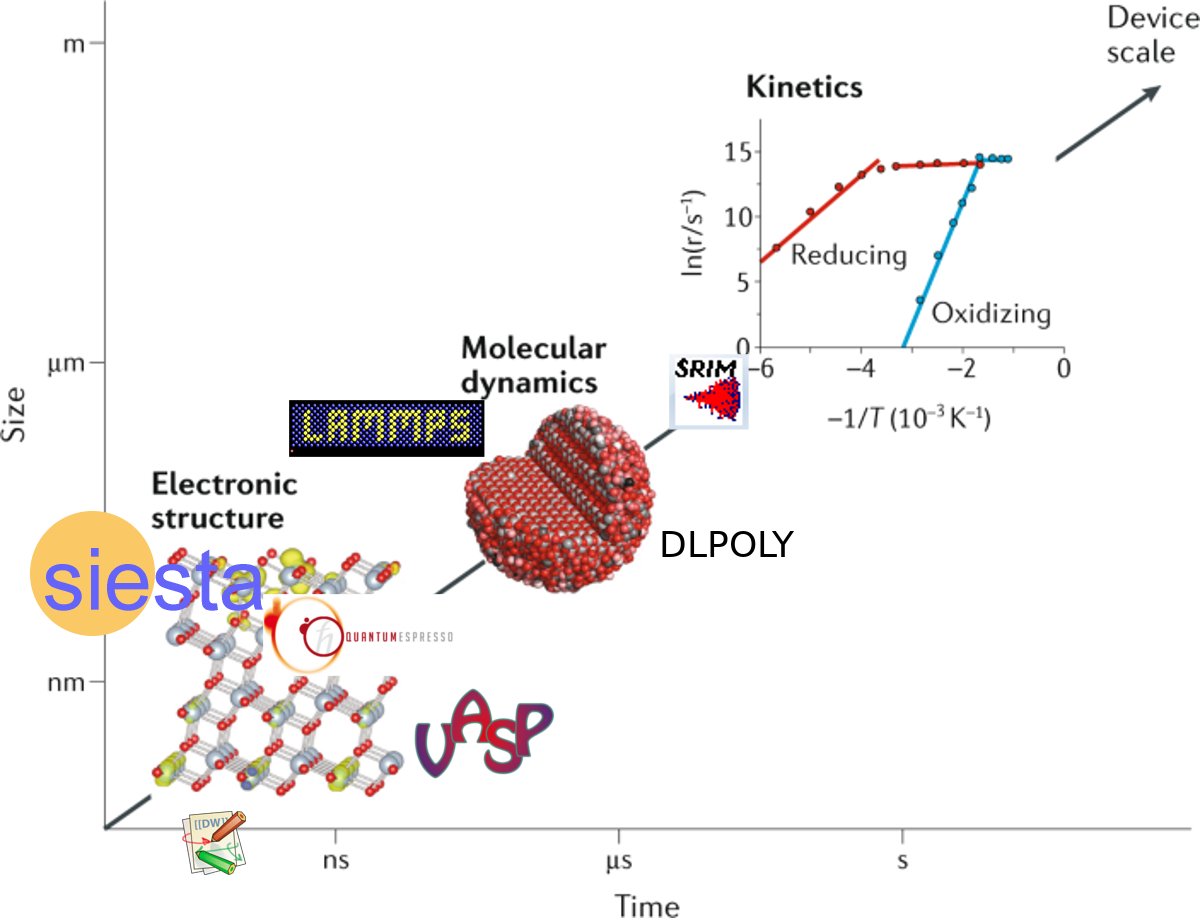
\includegraphics[width=10.0cm]{chapters/interatomic_potential_fitting/images/scale.png}
    \captionsetup{font={it}}
    \caption{Time and Size Scales for Computer Packages \cite{scalediagram}}
    \label{fig:timesizascalesmodelling}
  \end{center}
\end{figure}

The properties of metals may be approximated using small crystals rather than the whole grain, and this is ideally suited to \acrshort{dft} calculations.  Simulations of small ensembles of atoms over time are now also possible using \acrshort{dft} molecular dynamics.  Larger simulations containing thousands to millions of atoms, that are able to simulate single damage cascades are suitable for \acrshort{md} simulations (fig. \ref{fig:timesizascalesmodelling}). 




%%%%%%%%%%%%%%%%%%%%%%%%%%%%%%%%%%%%%%%%%%%%%%%%%%%%%%%%%%%%%%%%%%%%%%%%%%%%%%%%%%%%%%%%%%%%%%%%%%%%%%%%%%
%%
%%  Properties of Crystals
%%
%%%%%%%%%%%%%%%%%%%%%%%%%%%%%%%%%%%%%%%%%%%%%%%%%%%%%%%%%%%%%%%%%%%%%%%%%%%%%%%%%%%%%%%%%%%%%%%%%%%%%%%%%%

\section{Properties of Crystals}

\subsection{Introduction}

There are seven crystal classes (table. \ref{table:crystalclasses}) and 14 Bravias lattices (section \ref{section:crystalsrecipbloch}), although this work is primarily concerned with cubic and \gls{orthorhombic} crystals.    

\begin{table}[h]
\begin{center}
\renewcommand{\arraystretch}{1.2}
\begin{tabular}{c c c}
\hline\hline
Class & Lengths & Angles \\
\hline\hline
Cubic & $a = b = c$ & $ \alpha = \beta = \gamma = 90^{\circ}$ \\
Hexagonal & $a = b, c $ & $ \alpha = \beta, \gamma = 120^{\circ}$ \\
Rhombohedral & $a = b = c $ & $ \alpha = \beta = \gamma \neq 90^{\circ}$ \\
Tetragonal & $a = b, c $ & $ \alpha = \beta = \gamma = 90^{\circ}$ \\
Orthorhombic & $a, b, c $ & $ \alpha = \beta = \gamma = 90^{\circ}$ \\
Monoclinic & $a, b, c $ & $ \alpha = \beta = 90^{\circ}, \gamma \neq 90^{\circ} $ \\
Triclinic & $a, b, c $ & $ \alpha, \beta, \gamma, $ \\
\hline\hline
\end{tabular}
\caption{Seven Crystal Classes}
\label{table:crystalclasses}
\end{center}
\end{table}

Metals are rarely single crystals, but are made from many crystals separated by grain boundaries.  However, the knowledge of the microscopic crystals translates well to the properties of the metals on a macroscopic scale.

This work does not attempt to calculate properties based on a collection of many crystals, but on a single crystal with less that a thousand atoms.  The crystals are then assumed to be infinite in size, due to periodic boundary conditions.



\subsection{Equation of State}

The equation of state relates two or more intensive thermodynamic parameters.  In this work, the parameters of interest are the energy and volume of a system and the equation of state that connects them.  Knowing this not only allows one to predict the energy or pressure at a certain volume, but also the minimum energy, relaxed volume and the bulk modulus.  Being able to determine these equations for materials will be important when fitting interatomic potentials as they will be used to contribute to measuring how well the model, using the derived potentials, matches either \acrshort{dft} or experimental values.

\subsubsection{Bulk Modulus}

The bulk modulus of a material is defined as the bulk stress of a sample divided by the bulk strain on that sample and several example values are given in table \ref{table:examplebulkmodulii}.  It is also the inverse of the compressibility of that material, which means that materials with a higher bulk modulus are less compressible than those with a lower value.

\begin{equation}
  \begin{split}
  B_{0} = -V \frac{\partial P}{\partial V}
  \end{split}
  \label{eq:eqBulkModulusA}
\end{equation}

\begin{equation}
  \begin{split}
  B_{0} = V \frac{\partial^2 E}{\partial V^2}
  \end{split}
  \label{eq:eqBulkModulusB}
\end{equation}

The bulk modulus ($B_0$) may be calculated using the change in pressure ($P$) with respect to volume ($V$), as given in eq. \ref{eq:eqBulkModulusA}.  It may also be computed using the second derivative of the energy ($E$) with respect to volume (eq. \ref{eq:eqBulkModulusB}). 

\begin{table}[h]
\begin{center}
\renewcommand{\arraystretch}{1.2}
\begin{tabular}{c c}
\hline\hline
Material & Bulk Modulus/GPa \\
\hline\hline
Aluminium & 70 \\
Iron (BCC) & 110 \\
Stainless Steel 18-8 & 163 \\
\hline\hline
\end{tabular}
\end{center}
\caption{Example bulk modulii for three metals}
\label{table:examplebulkmodulii}
\end{table}

\subsubsection{Murnaghan Equation of State}

Hooke's law implies a linear relationship between stress and strain.  In practice, where a pressure is applied to a material, the application of Hooke's law is limited.  Muraghan derived a new equation\cite{murnaghaneq} to improve upon formulae developed in the 1930's, using compression data from high pressure experiments.

\begin{equation}
\begin{split}
P(V) = \frac{B_0}{{B'}_0}\left(\left(\frac{V_0}{V}\right)^{{B'}_0}-1\right)
\end{split}
\label{eq:eqMurnachanEquationofStatePressure}
\end{equation}

As pressure is the negative derivative of the internal energy of the system with respect to change in volume, $P = -(\partial E/dV)$ (eq. \ref{eq:eqMurnachanEquationofStatePressure}, the equation can be integrated and written in terms of the energy, volume, bulk modulus and its derivative (${B'}_0$)\cite{crystaleos}.

\begin{equation}
\begin{split}
E(V) = E_0 + \frac{B_0 V}{{B'}_0} \left[\left(\frac{V_0}{V}\right)^{{B'}_0} \frac{1}{{B'}_0 - 1} + 1 \right] - \frac{B_0 V_0}{{B'}_0-1}
\end{split}
\label{eq:eqMurnachanEquationofStateEnergy}
\end{equation}

The relaxed energy ($E_0$) and relaxed volume ($V_0$) are also required and the result is given in eq. \ref{eq:eqMurnachanEquationofStateEnergy}.

\subsubsection{Birch-Murnaghan Equation of State}

Several years after Murnaghan's equation, Birch developed the equation of state (eq. \ref{eq:eqBMEoS}) further upon the experimental data provided by work from Bridgman in high pressure physics.  For cubic symmetry, the description of free energy now includes third order terms in the strain components\cite{birchmurnaghaneq}.

\begin{equation}
\begin{split}
P(V) = \frac{3 B_0}{2} \left[\left(\frac{V_0}{V}\right)^{\frac{7}{3}}-\left(\frac{V_0}{V}\right)^{\frac{5}{3}}\right] \left[1 + \frac{3}{4}({B'}_0-4)\left(\left(\frac{V_0}{V}\right)^{\frac{2}{3}}-1\right)\right]
\end{split}
\label{eq:eqBMEoS}
\end{equation}

The energy-volume relationship may again be constructed\cite{crystaleos} (eq. \ref{eq:eqBMEoS2}).

\begin{equation}
\begin{split}
E(V) = E_0 + \frac{9 V_0 B_0}{16} \left[ \left[ \left(\frac{V_0}{V} \right)^{\frac{2}{3}}-1\right]^{3} {B'}_0 + \left[ \left(\frac{V_0}{V} \right)^{\frac{2}{3}}-1\right]^{2} \left[6 - 4 \left(\frac{V_0}{V} \right)^{\frac{2}{3}}\right] \right]
\end{split}
\label{eq:eqBMEoS2}
\end{equation}

In order to fit the Birch-Murnaghan, the first step is to fit a second order polynomial to the energy-volume data.  This may be achieved using least-squares fitting with a Vandermonde matrix.  The coefficients from this polynomial may then be used to calculate reasonable values for $E_0$, $V_0$ and $B_0$; sane starting values of ${B'}_0$ are between 1 and 10, and a recommended value in the literature is 2\cite{gilgamesheos}.

\begin{equation}
\begin{split}
E(V) = c_0 + c_1 V + c_2 V^2 \\
V_0 = -\frac{c_1}{2c_2} \\
E_0 = c_2 \times {V_0}^2 + c_1 V_0 + c_0  \\
B_0 = 2 c_2 V_0 \\
{B'}_0 = 2
\end{split}
\label{eq:eqMurnachanEquationofStateVolume}
\end{equation}

A suitable optimization algorithm (Newton-Raphson, Newton-Gauss, \acrshort{bfgs}) may then be used to attempt to minimise the fit further for $E_0$, $V_0$ and $B_0$ whilst trying values of ${B'}_0 \in {1.0,1.5,2.0,2.5,3.0,3.5,4.0,4.5,5.0,5.5,6.0}$.  The parameters with the lowest residual square sum are returned.

Mehl et al used a version of the Birch equation of state\cite{birchmurnaghaneq} and suggest a value for ${B'}_0$ between 3 and 5\cite{mehlsp} and limit the value of N in eq. \ref{eq:eqBirchMehlEtAl} to either 3 or 4 for the best data fit.

\begin{equation}
\begin{split}
E(V) = E_0 + \frac{9}{8} B_0 V_0 \left[ \left(\frac{V_0}{V}\right)^{\frac{2}{3}} - 1 \right]^{2} + \frac{9}{16} B_0(B_0^{'} - 4) V_0 \times \left[ \left(\frac{V_0}{V}\right)^{\frac{2}{3}} - 1 \right]^{3} + \sum_{n=4}^{N} \gamma_n \left[ \left(\frac{V_0}{V}\right)^{\frac{2}{3}} - 1 \right]^{n}
\end{split}
\label{eq:eqBirchMehlEtAl}
\end{equation}

In generating the data for a Birch or Birch-Murnaghan fit the atom configuration is relaxed.  A small strain $\left[\sigma, \sigma, \sigma, 0.0, 0.0, 0.0\right]$ is applied to decrease and increase the volume slightly about the relaxed volume.


\FloatBarrier
\subsubsection{Rose-Vinet Equation of State}
\label{section:rosevineteos}

More recently a Universal form, eq \ref{eq:eqRoseVinet}, was proposed by Rose, Vinet et al\cite{rosevinet}\cite{bonnywre}.  With an exponential cut off, this fits from the relaxed lattice parameter to much wider separations with a good fit for simple and transition metals, including K, Mo, Cu (fig. \ref{fig:rosevinet}).

\begin{equation}
\begin{split}
E(a) = E_0 + \left(1 + -\alpha \left(\frac{a}{a_0 - 1}\right)\right) \exp\left(-\alpha \left(\frac{a}{a_0 - 1}\right)\right) \\ 
\alpha = \sqrt{\frac{9 \Omega B_0}{-E0}}
\end{split}
\label{eq:eqRoseVinet}
\end{equation}

The energy ($E(a)$) is dependent upon the lattice parameter ($a$).  The relaxed lattice parameter ($a_0$), cohesive energy ($E_0$), atomic volume of the relaxed primitive cell ($\Omega$) and bulk modulus ($B_0$) are required for this equation of state.

\begin{figure}[htbp]
  \begin{center}
    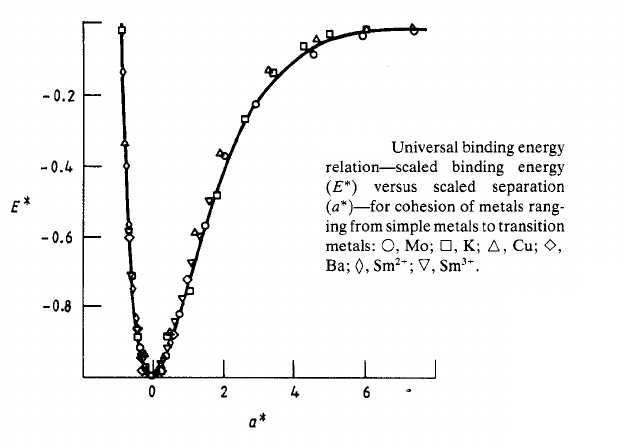
\includegraphics[width=.5\linewidth]{chapters/interatomic_potential_fitting/images/rosevinet.png}%
    \caption{Rose-Vinet Equation of State\cite{rosevinet}}
    \label{fig:rosevinet}
  \end{center}
\end{figure}

This has been used as a tool to fit interatomic potentials in work by Jelinek et al\cite{meamalsibaskes} and Bonny et al\cite{ipbonny}.  The version of the equation in this work is that used by Bonny et al and their fitting code, which will be discussed in more detail in section \ref{section:fittingprograms}.



\FloatBarrier
\subsection{Voigt Notation}

Where a tensor is symmetric, Voigt notation is used to simplify how the tensor is written.  It reduces a second order tensor such as stress or strain, represented by a 3x3 matrix, to a 6 row matrix.  It also reduces a fourth order tensor, such as the compliance or stiffness tensor (represented by a 3x3x3x3 matrix), to a 6x6 matrix. 


\begin{equation}
\begin{split}
\vec{A} =
\begin{bmatrix}
A_{11} & A_{12} & A_{13}   \\
A_{21} & A_{22} & A_{23}   \\
A_{31} & A_{32} & A_{33}   \\
\end{bmatrix}
= 
\begin{bmatrix}
A_{11} \\
A_{22} \\
A_{33} \\
A_{23} \\
A_{13} \\
A_{12} \\
\end{bmatrix}
\textnormal{  if } \vec{A}  \textnormal{ is symmetric }
\end{split}
\label{eq:voigtexample}
\end{equation}



\subsection{Elastic Constants}

Stress and strain are both related by either the stiffness tensor $C$, filled with the elastic constants, or the compliance tensor $S$ and this is the inverse of the stiffness tensor.  Strain is a measure of the deformation of a material and by definition has no units.  In one dimension $\epsilon = \frac{\delta l}{l_0}$ where $\l_0$ is the unstrained length and $\delta l$ is the change in length.  The Generalized Hooke's law relating these tensors allows the computation of the Cauchy stress if the elastic constants are known and an input strain is provided.

\begin{equation}
\begin{split}
\vec{A} =
\begin{bmatrix}
\epsilon_{11} & \epsilon_{12} & \epsilon_{13}   \\
\epsilon_{21} & \epsilon_{22} & \epsilon_{23}   \\
\epsilon_{31} & \epsilon_{32} & \epsilon_{33}   \\
\end{bmatrix} = \begin{bmatrix}
\epsilon_{11} \\
\epsilon_{22} \\
\epsilon_{33} \\
\epsilon_{23} \\
\epsilon_{13} \\
\epsilon_{12} \\
\end{bmatrix}
\textnormal{ where }
\epsilon{ij} \equiv \frac{1}{2} \left(\frac{\partial u_i}{\partial x_j} + \frac{\partial u_j}{\partial x_i}\right)
\end{split}
\label{eq:strainTensor}
\end{equation}


\begin{equation}
  \begin{split}
    \vec{\sigma_{ij}} = \vec{C_{ijkl}} \vec{\epsilon_{kl}} 
  \end{split}
  \label{eq:eqStiffnessTensor}
\end{equation}


\begin{equation}
  \begin{split}
    \vec{\epsilon_{ij}} = \vec{S_{ijkl}} \vec{\sigma_{kl}} 
  \end{split}
  \label{eq:eqStiffnessTensor}
\end{equation}

\eqStrainTensorVoight

\begin{equation}
  \begin{split}
    \begin{bmatrix}
      \sigma_{1} \\
      \sigma_{2} \\
      \sigma_{3} \\
      \sigma_{4} \\
      \sigma_{5} \\
      \sigma_{6} \\
      \end{bmatrix} = \begin{bmatrix}
      C_{11} & C_{12} & C_{13} & C_{14} & C_{15} & C_{16} \\
      C_{21} & C_{22} & C_{23} & C_{24} & C_{25} & C_{26} \\
      C_{31} & C_{32} & C_{33} & C_{34} & C_{35} & C_{36} \\
      C_{41} & C_{42} & C_{43} & C_{44} & C_{45} & C_{45} \\
      C_{51} & C_{52} & C_{53} & C_{54} & C_{55} & C_{55} \\
      C_{61} & C_{62} & C_{63} & C_{64} & C_{65} & C_{66} \\
      \end{bmatrix} \begin{bmatrix}
      \epsilon_{1} \\
      \epsilon_{2} \\
      \epsilon_{3} \\
      \epsilon_{4} \\
      \epsilon_{5} \\
      \epsilon_{6} \\
      \end{bmatrix}\\
    \end{split}
    \label{eq:eqelasticconstants}
\end{equation}

There are 81 elastic constants, although as the tensor is symmetric it may be written in Voigt notation with 36 values (eq. \ref{eq:eqelasticconstants}).  The number of independent elastic constants may be reduced further depending on the symmetry of the crystal.  The tensors in Voigt notation are given for cubic, orthorhombic/orthotropic, monoclinic and triclinic in appendix \ref{section:elasticconstantsappendix}.


\subsection{Calculating Elastic Constants for a Cubic Crystal}

Cubic crystals are the most simple class with primitive unit cells having three orthonormal basis vectors.  Four of the most common variants of the cubic crystal are the simple cubic, \acrlong{bcc}, \acrlong{fcc} and zincblende.  Due to symmetry, a cubic crystal has only three elastic independent constants; in Voigt notation these are $C_{11}$, $C_{12}$ and $C_{44}$.

Applying two strains to a cubic crystal \cite{pressuredepmehl} coupled with the calculation of the bulk modulus, as already discussed, allows the three independent elastic constants to be calculated.

First, the bulk modulus may be calculated either by finding the second derivative of the energy wrt volume at the relaxed volume, $B(V) = -V P'(V) = V E''(V)$\cite{pressuredepmehl}, or by fitting the Birch-Murnaghan equation of state.

\begin{equation}
  \begin{split}
    \epsilon_{(C11 - C22)} = 
    \begin{bmatrix}
    \delta & 0 & 0   \\
    0 & - \delta & 0   \\
    0 & 0 & \delta^2 / (1 - \delta^2)   \\
    \end{bmatrix}
  \end{split}
  \label{eq:volConserveOrtho}
\end{equation}

Second, a volume conserving orthorhombic strain (eq. \ref{eq:volConserveOrtho}) may be applied to the crystal \cite{pressuredepmehl}.  The relation between the relaxed energy and that under strain is symmetric about $E(0)$ and is given by $E(\delta) = E(-\delta) = E(0) + (C_{11} - C_{12}) V \delta^2 + O[\delta^4]$\cite{pressuredepmehl}.  $V$ is the volume of the relaxed unit cell and $E(0)$ is the minimum energy.  By fitting a polynomial to the energy-strain data, the coefficient for the quadratic term is equal to $(C_{11} - C_{12}) V$.

  \begin{equation}
    \begin{split}
      \epsilon_{(C44)} = 
      \begin{bmatrix}
      0 & \frac{\delta}{2} & 0   \\
       \frac{\delta}{2} & 0 & 0   \\
      0 & 0 & \delta^2 / (4 - \delta^2)   \\
      \end{bmatrix}
    \end{split}
    \label{eq:monoclinicstrain}
  \end{equation}

Third, a volume conserving monoclinic strain (eq. \ref{eq:monoclinicstrain}) is applied and the relation between the relaxed energy, strained energy and the elastic constant $C_{44}$ is $E(\delta) = E(-\delta) = E(0) + \frac{1}{2} C_{44} V \delta^2 + O[\delta^4]$.  Similarly, fitting a polynomial to the strain-energy data points will calculate the value of $C_{44}$.

Finally, the relation between the bulk modulus, $C_{11}$ and $C_{12}$, $B_0 = (C_{11} + 2 C_{12}) / 3$ allows the computation of the individual constants eq. \ref{eq:c11c12elastic} (this relationship is only for cubic crystals).

\begin{equation}
\begin{split}
C_{ortho} = C_{11} - C_{12} \\
C_{11} = \frac{3B_0 + 2 C_{ortho}}{3} \\
C_{12} = \frac{3B_0 - C_{ortho}}{3}
\end{split}
\label{eq:c11c12elastic}
\end{equation}



\subsection{Calculating Elastic Constants for Orthorhombic Crystal}
\label{section:calcelasticconstants}

The \acrshort{dft} work here includes Fe, Ru and Pd.  Pure iron at room temperature is \acrshort{bcc}, but this work is interested in austenetic stainless steel where the structure of atoms in the alloy are \acrshort{fcc}.  When modelling \acrshort{fcc} iron using \acrshort{dft} with a non-polarized calculation, the crystal favours a cubic crystal with the atoms fixed in the \acrshort{fcc} positions.  When a spin-polarized calculation is computed, with magnetization along the z-axis, the crystal becomes slightly tetragonal with one side being 5\% larger than the other two.  This is a non-cubic crystal and the approach by Mehl et al to compute elastic constants is not applicable.


%\begin{center}
%\begin{tikzpicture}[scale=0.5]
%\printtikzcrystalbcccubic{}
%\end{tikzpicture} 
%\begin{tikzpicture}[scale=0.5]
%\printtikzcrystalbcccubic{}
%\end{tikzpicture} 
%\end{center}

\begin{equation}
    \begin{split}
      C_{ij} = 
      \begin{bmatrix}
      C_{11} & C_{12} & C_{12} & 0      & 0      & 0      \\
      C_{12} & C_{11} & C_{12} & 0      & 0      & 0      \\
      C_{12} & C_{12} & C_{11} & 0      & 0      & 0      \\
      0      & 0      & 0      & C_{44} & 0      & 0      \\
      0      & 0      & 0      & 0      & C_{44} & 0      \\
      0      & 0      & 0      & 0      & 0      & C_{44} \\
      \end{bmatrix}\\
      \text{(3 independent values)}
    \end{split}
  \label{eq:eqCubicEC}
\end{equation}


\begin{equation}
    \begin{split}
      C_{ij} = 
      \begin{bmatrix}
      C_{11} & C_{12} & C_{13} & 0      & 0      & 0      \\
      C_{12} & C_{22} & C_{23} & 0      & 0      & 0      \\
      C_{13} & C_{23} & C_{33} & 0      & 0      & 0      \\
      0      & 0      & 0      & C_{44} & 0      & 0      \\
      0      & 0      & 0      & 0      & C_{55} & 0      \\
      0      & 0      & 0      & 0      & 0      & C_{66} \\
      \end{bmatrix}\\
      \text{(9 independent values)}
    \end{split}
    \label{eq:eqOrthoRhombicEC}
\end{equation}


Once the relaxed crystal basis vectors and atom positions have been determined for the orthorhombic crystal, nine strains are applied to the crystal \cite{dftrfkj} in order to calculate the nine independent elastic constants.


\FloatBarrier

As a strain is applied to a crystal its energy can change.  The volume may also change, although it may be held constant.  The relationship between the energy and the strain $\sigma$ may be represented as a Taylor expansion of the internal energy in powers of the strain tensor\cite{dftrfkj}.  The equation used by Ravindran et al is in a slightly different notation to that used by Mehl\cite{elasticpropertiesmehl}.  It includes a constant $\xi$ to account for the symmetry of $\sigma$ and the use of Voigt notation.

\begin{equation}
  \begin{split}
  E(V,\sigma) = E(V_{0},0) + V_{0} \left( \sum_{i} \tau_i \xi_i \sigma_i + \frac{1}{2} \sum_{ij} c_{ij} \sigma_{i} \xi_{i} \sigma_{j} \xi_{j} \right) + O(\sigma^3) \\
\text{where } \sigma \text{ is the strain} \\
\text{and } \tau \text{ is the stress} \\
\text{if the index } k \text{ of } \xi \text{ is } \in {1, 2, 3} \text{ then } \xi_k = 1 \\
\text{if the index } k \text{ of } \xi \text{ is } \in {4, 5, 6} \text{ then } \xi_k = 2 \\
  \end{split}
\end{equation}


The first three strains applied to the orthorhombic crystal are non-volume conserving.  They strain the crystal along each axis and allow the calculation of $C_{11}$, $C_{22}$ and $C_{33}$.


%% D1

\begin{center}
\begin{minipage}{.35\textwidth}
  \begin{equation}
    \begin{split}
      D_{1} = 
      \begin{bmatrix}
      1 + \delta & 0       & 0             \\
      0          & 1       & 0             \\
      0          & 0       & 1             \\
      \end{bmatrix}
    \end{split}
  \label{eq:distortion1}
  \end{equation}
\end{minipage}
\begin{minipage}{.10\textwidth}
\end{minipage}
\begin{minipage}{.54\textwidth}
  \begin{equation}
    \begin{split}
    E(V,\sigma) = E(V_{0},0) + V_{0} \left( \tau_{1} \sigma + \frac{c_{11}}{2} \sigma^2 \right)
    \end{split}
  \label{eq:distortion1energy}
  \end{equation}
\end{minipage}
\end{center}

%% D2

\begin{center}
\begin{minipage}{.35\textwidth}
  \begin{equation}
    \begin{split}
      D_{2} = 
      \begin{bmatrix}
      1          & 0           & 0             \\
      0          & 1 + \delta  & 0             \\
      0          & 0           & 1             \\
      \end{bmatrix}
    \end{split}
  \label{eq:distortion2}
  \end{equation}
\end{minipage}
\begin{minipage}{.10\textwidth}
\end{minipage}
\begin{minipage}{.54\textwidth}
  \begin{equation}
    \begin{split}
    E(V,\sigma) = E(V_{0},0) + V_{0} \left( \tau_{2} \sigma + \frac{c_{22}}{2} \sigma^2 \right)
    \end{split}
  \label{eq:distortion2energy}
  \end{equation}
\end{minipage}
\end{center}

%% D3

\begin{center}
\begin{minipage}{.35\textwidth}
  \begin{equation}
    \begin{split}
      D_{3} = 
      \begin{bmatrix}
      1          & 0           & 0             \\
      0          & 1           & 0             \\
      0          & 0           & 1 + \delta    \\
      \end{bmatrix}
    \end{split}
  \label{eq:distortion3}
  \end{equation}
\end{minipage}
\begin{minipage}{.10\textwidth}
\end{minipage}
\begin{minipage}{.54\textwidth}
  \begin{equation}
    \begin{split}
    E(V,\sigma) = E(V_{0},0) + V_{0} \left( \tau_{3} \sigma + \frac{c_{33}}{2} \sigma^2 \right)
    \end{split}
  \label{eq:distortion3energy}
  \end{equation}
\end{minipage}
\end{center}

Volume conserving monoclinic distortions (eq. \ref{eq:distortion4}, eq. \ref{eq:distortion5}, eq. \ref{eq:distortion6}) are used to calculate the $C_{44}$, $C_{55}$ and $C_{66}$ elastic constants (eq. \ref{eq:distortion4energy}, eq. \ref{eq:distortion5energy}, eq. \ref{eq:distortion6energy}).


%% D4

\begin{center}
\begin{minipage}{.35\textwidth}
  \begin{equation}
    \begin{split}
      D_{4} = 
      \begin{bmatrix}
      \frac{1}{(1-\sigma^2)^{\frac{1}{3}}} & 0           & 0             \\
      0                                    & \frac{1}{(1-\sigma^2)^{\frac{1}{3}}}      & \frac{\sigma}{(1-\sigma^2)^{\frac{1}{3}}}  \\
      0                                    & \frac{\sigma}{(1-\sigma^2)^{\frac{1}{3}}} & \frac{1}{(1-\sigma^2)^{\frac{1}{3}}}       \\
      \end{bmatrix}
    \end{split}
  \label{eq:distortion4}
  \end{equation}
\end{minipage}
\begin{minipage}{.10\textwidth}
\end{minipage}
\begin{minipage}{.54\textwidth}
  \begin{equation}
    \begin{split}
    E(V,\sigma) = E(V_{0},0) + V_{0} \left(2 \tau_{4} \sigma + 2 \frac{c_{44}}{2} \sigma^2 \right)
    \end{split}
  \label{eq:distortion4energy}
  \end{equation}
\end{minipage}
\end{center}

%% D5

\begin{center}
\begin{minipage}{.35\textwidth}
  \begin{equation}
    \begin{split}
      D_{5} = 
      \begin{bmatrix}
      \frac{1}{(1-\sigma^2)^{\frac{1}{3}}} & 0           & \frac{\sigma}{(1-\sigma^2)^{\frac{1}{3}}}              \\
      0                                    & \frac{1}{(1-\sigma^2)^{\frac{1}{3}}}      &   0  \\
      \frac{\sigma}{(1-\sigma^2)^{\frac{1}{3}}}   &   0  & \frac{1}{(1-\sigma^2)^{\frac{1}{3}}}       \\
      \end{bmatrix}
    \label{eq:distortion5}
    \end{split}
  \end{equation}
\end{minipage}
\begin{minipage}{.10\textwidth}
\end{minipage}
\begin{minipage}{.54\textwidth}
  \begin{equation}
    \begin{split}
    E(V,\sigma) = E(V_{0},0) + V_{0} \left(2 \tau_{5} \sigma + 2 \frac{c_{55}}{2} \sigma^2 \right)
    \end{split}
  \label{eq:distortion5energy}
  \end{equation}
\end{minipage}
\end{center}

%% D6

\begin{center}
\begin{minipage}{.39\textwidth}
  \begin{equation}
    \begin{split}
      D_{6} = 
      \begin{bmatrix}
      \frac{1}{(1-\sigma^2)^{\frac{1}{3}}}        & \frac{\sigma}{(1-\sigma^2)^{\frac{1}{3}}} & 0   \\
      \frac{\sigma}{(1-\sigma^2)^{\frac{1}{3}}}   & \frac{1}{(1-\sigma^2)^{\frac{1}{3}}}      &   0  \\
      0                                           & 0                                         & \frac{1}{(1-\sigma^2)^{\frac{1}{3}}}       \\
      \end{bmatrix}
    \end{split}
  \label{eq:distortion6}
  \end{equation}
\end{minipage}
\begin{minipage}{.04\textwidth}
\end{minipage}
\begin{minipage}{.56\textwidth}
  \begin{equation}
    \begin{split}
    E(V,\sigma) = E(V_{0},0) + V_{0} \left(2 \tau_{6} \sigma + 2 \frac{c_{66}}{2} \sigma^2 \right)
    \end{split}
  \label{eq:distortion6energy}
  \end{equation}
\end{minipage}
\end{center}


Finally, three orthorhombic strains (eq. \ref{eq:distortion7}, eq. \ref{eq:distortion8}, eq. \ref{eq:distortion9}) that conserve the volume, by altering the strain along each axis, are used to calculate the $C_{12}$, $C_{13}$ and $C_{23}$ elastic constants (eq. \ref{eq:distortion7energy}, eq. \ref{eq:distortion8energy}, eq. \ref{eq:distortion9energy}).



%% D7

\begin{center}
\begin{minipage}{.39\textwidth}
  \begin{equation}
    \begin{split}
      D_{7} = 
      \begin{bmatrix}
      \frac{1 + \sigma}{(1-\sigma^2)^{\frac{1}{3}}} & 0           & 0              \\
      0                                    & \frac{1 - \sigma}{(1-\sigma^2)^{\frac{1}{3}}}      &   0  \\
      0  &   0  & \frac{1}{(1-\sigma^2)^{\frac{1}{3}}}       \\
      \end{bmatrix}
    \end{split}
  \label{eq:distortion7}
  \end{equation}
\end{minipage}
\begin{minipage}{.04\textwidth}
\end{minipage}
\begin{minipage}{.56\textwidth}
  \begin{equation}
    \begin{split}
    E(V,\sigma) = E(V_{0},0) + V_{0} \left((\tau_{1}-\tau{2} \sigma + \frac{1}{2} (c_{11} + c_{22} - 2 c_{12}) \sigma^2 \right)
    \end{split}
  \label{eq:distortion7energy}
  \end{equation}
\end{minipage}
\end{center}

%% D8

\begin{center}
\begin{minipage}{.4\textwidth}
  \begin{equation}
    \begin{split}
      D_{8} = 
      \begin{bmatrix}
      \frac{1 + \sigma}{(1-\sigma^2)^{\frac{1}{3}}} & 0           & 0              \\
      0                                    & \frac{1}{(1-\sigma^2)^{\frac{1}{3}}}      &   0  \\
      0  &   0  & \frac{1-\sigma}{(1-\sigma^2)^{\frac{1}{3}}}       \\
      \end{bmatrix}
    \end{split}
  \label{eq:distortion8}
  \end{equation}
\end{minipage}
\begin{minipage}{.02\textwidth}
\end{minipage}
\begin{minipage}{.58\textwidth}
  \begin{equation}
    \begin{split}
    E(V,\sigma) = E(V_{0},0) + V_{0} \left((\tau_{1}-\tau{3} \sigma + \frac{1}{2} (c_{11} + c_{33} - 2 c_{13}) \sigma^2 \right)
    \end{split}
  \label{eq:distortion8energy}
  \end{equation}
\end{minipage}
\end{center}

%% D9

\begin{center}
\begin{minipage}{.4\textwidth}
  \begin{equation}
    \begin{split}
      D_{9} = 
      \begin{bmatrix}
      \frac{1}{(1-\sigma^2)^{\frac{1}{3}}} & 0           & 0              \\
      0  & \frac{1 + \sigma}{(1-\sigma^2)^{\frac{1}{3}}}      &   0  \\
      0  &   0  & \frac{1 - \sigma}{(1-\sigma^2)^{\frac{1}{3}}}       \\
      \end{bmatrix}
    \end{split}
  \label{eq:distortion9}
  \end{equation}
\end{minipage}
\begin{minipage}{.02\textwidth}
\end{minipage}
\begin{minipage}{.58\textwidth}
  \begin{equation}
    \begin{split}
    E(V,\sigma) = E(V_{0},0) + V_{0} \left((\tau_{2}-\tau{3} \sigma + \frac{1}{2} (c_{22} + c_{33} - 2 c_{23}) \sigma^2 \right)
    \end{split}
  \label{eq:distortion9energy}
  \end{equation}
\end{minipage}
\end{center}


\FloatBarrier
\subsection{Stability Conditions and Other Properties}

Once the elastic constants are calculated, a number of other properties may be computed from them.  The stability of a crystal, bulk modulus, shear modulus and Young's modulus may all be found from the elastic constants.  There is also a correlation between these and the melting temeperature of a material.  These are discussed in detail in appendix \ref{section:elasticconstantsappendix} and were implemented in the potential fitting code that results from this work.




\FloatBarrier
\section[Choice of Function]{Interatomic Potentials and Choice of Function}

\subsection{Introduction}

An interatomic potential, as used in this work and \acrshort{md} computer codes, is a function or a set of functions that describe the energy and force between atoms.  Simpler functions represent the potential energy between pairs of atoms only, but more complicated functions have been used in molecular dynamics since the 1980s that also attempt to represent the many body nature of materials, which applies in particular to metals.


\subsection{Pair Potentials}

A pair potential only considers individual pairs of nearby atoms, one pair at a time, and does not consider the effect of any other nearby atoms.  Where an alloy is being modelled, there will be a pair potential function for each element and element combination; 1 for a single element, 3 for a two element alloy, 6 for a three element alloy and so on ($n (n + 1) / 2$).


\FloatBarrier
\subsubsection{Lennard-Jones}
\label{section:LennardJones}

The Lennard-Jones potential (eq. \ref{eq:eqLennardJones})\cite{jonespot}, fig. \ref{fig:lennardjonespot}, was proposed in the 1920s and has both an attractive term and a repulsive term; the $(r_m/r)^{12}$ becomes much larger than the $(r_m/r)^6$ term at close distances, and this mimics the coulomb repulsion as two atoms are pushed closer together.  At larger separations, the attractive term dominates.

\begin{equation}
\begin{split}
V(r) = e \left(\left(\frac{r_m}{r}\right)^{12} - 2 \left(\frac{r_m}{r}\right)^6\right)
\end{split}
\label{eq:eqLennardJones}
\end{equation}

\begin{figure}[!htbp]
  \begin{center}
    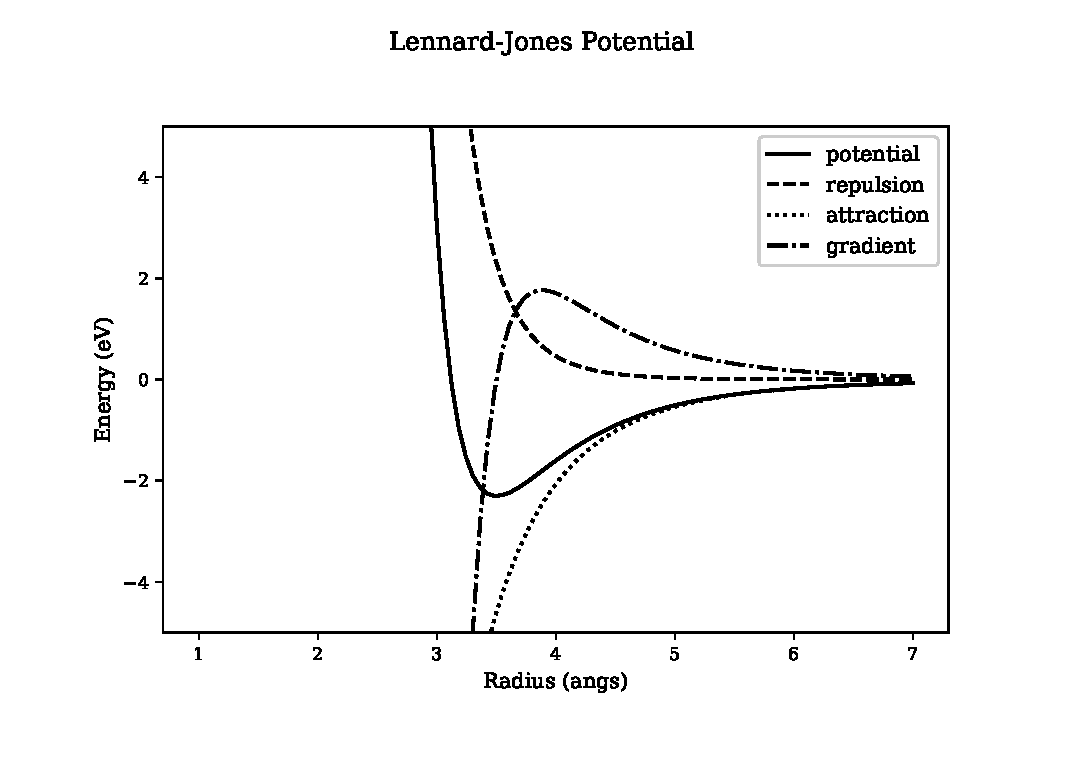
\includegraphics[width=.6\linewidth]{chapters/interatomic_potential_fitting/plots_pair_potentials/lennard_jones.eps}
    \caption{Lennard-Jones Potential}
    \label{fig:lennardjonespot}
  \end{center}
\end{figure}

The Lennard-Jones potential ($V(r)$) requires two parameters ($e$, $r_m$) and is dependent upon the atom separation ($r$).


\FloatBarrier
\subsubsection{Morse Potential}
\label{section:Morse}

The Morse potential (eq. \ref{eq:eqMorse})\cite{morsepot}, fig. \ref{fig:morsepot}, was proposed five years after the Lennard-Jones potential.  It also has an attractive and repulsive term, but it uses the exponential function rather than 6th and 12th powers.

\begin{equation}
\begin{split}
V(r) = \exp(-2 a (r - re)) - 2 \exp (-a(r - re))
\end{split}
\label{eq:eqMorse}
\end{equation}

\begin{figure}[!htbp]
  \begin{center}
    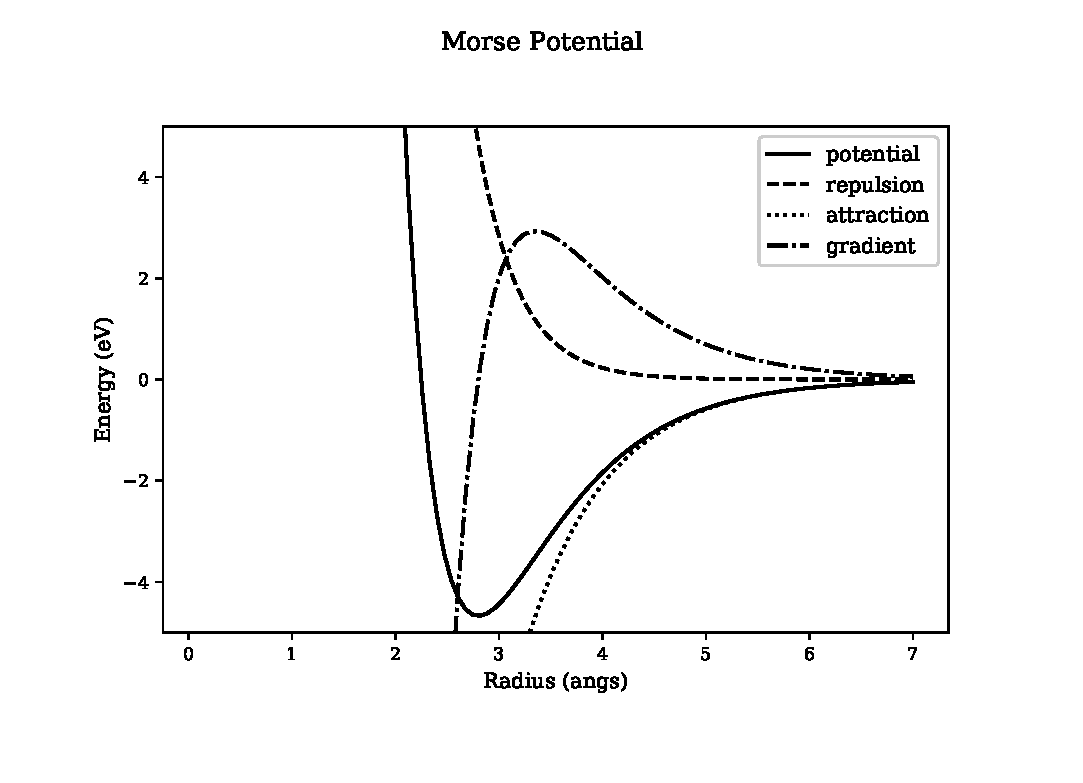
\includegraphics[width=.6\linewidth]{chapters/interatomic_potential_fitting/plots_pair_potentials/morse.eps}
    \caption{Morse Potential}
    \label{fig:morsepot}
  \end{center}
\end{figure}

The Morse potential ($V(r)$) requires two parameters ($a$, $r_e$) and is dependent upon the atom separation ($r$). 

\FloatBarrier
\subsubsection{Buckingham Potential}
\label{section:Buckingham}

The Buckingham Potential (eq. \ref{eq:eqBuckinghamPotential})\cite{buckpot} consists of a repulsive and attractive part.  As the separation decreases, the attractive term dominates and the overall functions tends towards negative infinity.  This shouldn't be problematic when gasses or solids are being modelled alone, but when collisions and damage cascades are being modelled, the separation between atoms may be much smaller than that in a typical simulation, ending with these atoms being pulled together (fig. \ref{fig:buckinghamplot}).

\begin{equation}
\begin{split}
V(r) = A \exp(-B  r) - \frac{C}{r^6}
\end{split}
\label{eq:eqBuckinghamPotential}
\end{equation}

\begin{figure}[!htbp]
  \begin{center}
    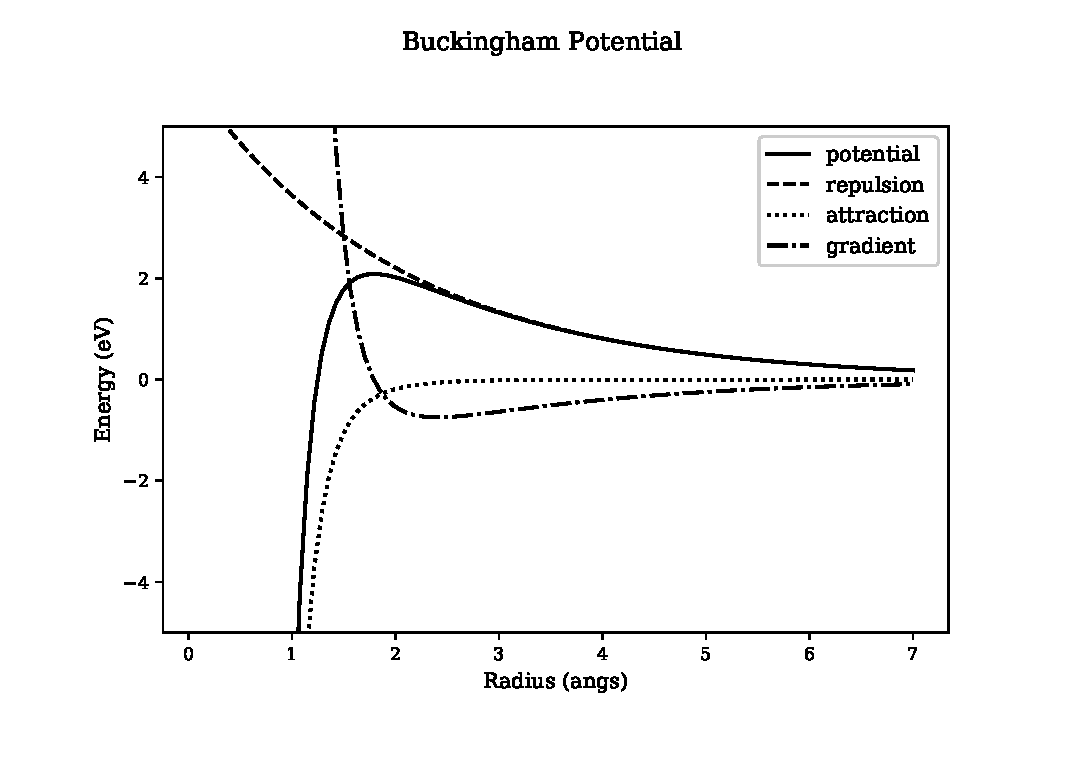
\includegraphics[width=.6\linewidth]{chapters/interatomic_potential_fitting/plots_pair_potentials/buckingham.eps}
    \caption{Buckingham Potential}
    \label{fig:buckinghamplot}
  \end{center}
\end{figure}

The Buckingham potential ($V(r)$) requires three parameters ($A$, $B$, $C$) and is dependent upon the atom separation ($r$).



\FloatBarrier
\subsubsection{\acrlong{zbl} Universal Potential Function}
\label{section:ZBL}

It became clear, while experimenting with a number of existing potentials and \acrshort{md} programs, that at the very least modifications to those potentials would need to be made for small atom separations.  A simulation to model a projectile failed early on due to the projectile's proximity to target atoms, resulting in the MD code returning an error as the separation was out of the range of the potential.

The \acrlong{zbl} (eq. \ref{eq:zblequation}) potential (fig. \ref{fig:zbluniversalscreening}), between an atom of charge $Z_i$ and $Z_j$ is set out in the \acrshort{srim} book\cite{srimbook}.


\begin{equation}
\begin{split}
V_{zbl}(r_{ij}, Z_i, Z_j) = \frac{1}{4 \pi \epsilon_0} \frac{Z_i Z_j}{r_{ij}} \phi \left( \frac{r_{ij}}{a_{ij}} \right) \\
\text{where } \epsilon_0 = 8.85419\times 10^{-12} 
\end{split}
\label{eq:zblequation}
\end{equation}

The parameters of the Universal screening potential $\phi \left( \frac{r_{ij}}{a_{ij}} \right)$ function are as follows:

\begin{equation}
\begin{split}
\phi(x) = 0.181 \exp({-3.2x}) + 0.5099 \exp({-0.9423x}) + 0.2802 \exp({-0.4028x}) + 0.02817 \exp({-0.2016x}) \\
\text{where } a_{ij} = \frac{0.8854 a_0}{Z^{\frac{2}{3}}_i + Z^{\frac{2}{3}}_j} \\
\text{and } a_0 = 0.529 \text{ angstrom (Bohr radius)}
\end{split}
\label{eq:screeningPotential}
\end{equation}

The Universal screening function has 8 parameters defined.  They do vary depending on the source, but these are as defined in the \acrshort{srim} 2015 book\cite{srimbook}.  The argument $x$ is equal to $\frac{r_{ij}}{a_{ij}}$ where $r_{ij}$ is the separation between atoms and $a_{ij}$ is the screening length defined by J. F. Ziegler, J. P. Biersack and M. D. Ziegler\cite{srimbook}.


\begin{figure}[!htbp]
  \begin{center}
    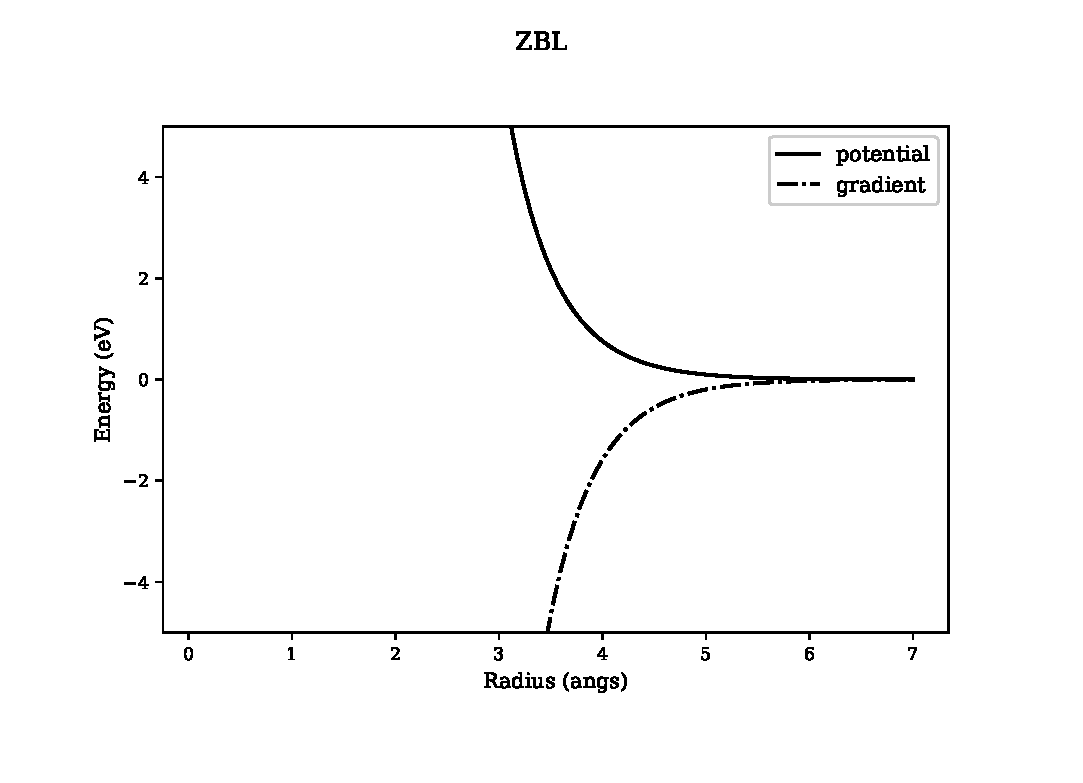
\includegraphics[width=.6\linewidth]{chapters/interatomic_potential_fitting/plots_pair_potentials/zbl.eps}
    \caption{\acrshort{zbl} universal screening potential}
    \label{fig:zbluniversalscreening}
  \end{center}
\end{figure}


\FloatBarrier




\subsection{Many Body Potentials}

This work is focused on metals, and two popular, and closely related potentials, will be discussed in this section.

\subsubsection{Finnis-Sinclair}
\label{section:FinnisSinclair}

The Finnis-Sinclair potential was published in 1984\cite{finnissinclair} and it introduced both a pair potential and an embedded term to take into account the cohesive energy dependent on the local electron density.  The pair term represents the repulsion between the atoms whereas the embedding functional glues the atoms together in the solid. 

\begin{equation}
\begin{split}
U_{total} = U_{P} + U_{N}
\end{split}
\label{eq:eqFinnisSinclairTotal}
\end{equation}

The tight-binding that this potential is based on is represented by the functional: square root of the density.  The potential for a single element model consists of a pair function (eq. \ref{eq:eqFinnisSinclairPair}), a density function and a tight-binding functional (eq. \ref{eq:eqFinnisSinclairEmbed}).

\begin{equation}
\begin{split}
U_P = \frac{1}{2} \sum_{ij} V(R_{ij}) \\
\end{split}
\label{eq:eqFinnisSinclairPair}
\end{equation}

\begin{equation}
\begin{split}
U_N = -A \sum_i f(\rho_i) \\
p_i = \sum_{j} \phi (R_{ij}) \\
\end{split}
\label{eq:eqFinnisSinclairEmbed}
\end{equation}

\begin{equation}
\begin{split}
R_{ij} = \abs{\vec{R_j} - \vec{R_i}}
\end{split}
\label{eq:eqAtomSeparation}
\end{equation}

The total energy ($U_{total}$) is the sum of the total pair ($U_P$) and total N-body terms ($U_{N}$).  Both the pair potential ($V(R_{ij})$) and electron density ($\phi(R_{ij})$) are dependent upon the atom separation distance (eq. \ref{eq:eqAtomSeparation}).  In the Finnis-Sinclair model, the embedded functional ($f(\rho_i)$) is chosen to be $\sqrt{\rho}$ in order to mimic tight-binding theory\cite{finnissinclair}. This functional is multiplied by a parameter ($A$), a value determined by the author of the potential.




\subsubsection{\Acrlong{eam}}
\label{section:EAM}

The \acrlong{eam} was also invented in the 1980s by Daw and Baskes\cite{dawbaskeseam} (eq. \ref{eq:eqEAM}).  It was developed with metals in mind, and in many ways is a more flexible variant of the Finnis-Sinclair potential.  It too has a pair and density function, but the functional of the \acrshort{eam} potential is not restricted to a square root.

\begin{equation}
\begin{split}
U_{EAM} = \frac{1}{2} \sum \limits_{i=1}^{N} \sum \limits_{j\ne i}^{N} V_{ij}(r_{ij}) + \sum \limits_{i=1}^{N} F[\rho _{i}] \\
\textnormal{where   } \rho_{i} = \sum \limits_{j=i,j \ne i}^{N} \rho_{ij}(r_{ij})
\end{split}
\label{eq:eqEAM}
\end{equation}

Elastic properties were not reliably calculated from pair functions alone\cite{dawbaskeseam}, but the advent of Finnis-Sinclair and \acrshort{eam} type potentials changed this.  

\begin{equation}
\begin{split}
A_{ij} + F'(\vec{\rho}) V_{ij} = 0 \\
\text{where} \\
A_{ij} = \frac{1}{2} \sum_{m} \phi'_m a_i^m a_j^m / a^m \\
V_{ij} = \frac{1}{2} \sum_{m} \rho'_m a_i^m a_j^m / a^m 
\end{split}
\label{eq:eqLatticeEquilib}
\end{equation}

For homonuclear cubic crystals, the lattice constant may be calculated by the equilibrium condition in eq \ref{eq:eqLatticeEquilib}.  The three independent elastic constants, $C_{11}, C_{12}, C_{44}$, may also be calculated at equilibrium from eq \ref{eq:eqCubicCrystalElastic}.  

\begin{equation}
\begin{split}
C_{11} = \left( B_{11} + F'(\vec{\rho}) W_{11} + F''(\vec{\rho})(V_{11})^2 \right) / \Omega_0 \\
C_{12} = \left( B_{12} + F'(\vec{\rho}) W_{12} + F''(\vec{\rho})(V_{11})^2 \right) / \Omega_0 \\
C_{44} = \left( B_{12} + F'(\vec{\rho}) W_{12} \right) / \Omega_0 \\
\text{where} \\
B_{ijkl} = \frac{1}{2} \sum_m \left(\phi''_m-\phi'_m/a^m \right) a_i^m a_j^m a_k^m a_l^m/(a^m)^2 \\
W_{ijkl} = \frac{1}{2} \sum_m \left(\rho''_m-\rho'_m/a^m \right) a_i^m a_j^m a_k^m a_l^m/(a^m)^2 \\
\text{where} \\
\phi''_m = \left(d^2\phi(r)/dr^2 \right)_{r=a^m,}\\
\rho''_m = \left(d^2\phi(r)/dr^2 \right)_{r=a^m.}\\
\end{split}
\label{eq:eqCubicCrystalElastic}
\end{equation}

There are notable consequences in removing either the pair function or embedding functional.  If $V_{ij}(r_{ij})$ is removed, $F'[\vec{\rho}] = 0$ and this gives a shear modulus of 0 ($C_{11} = C_{12}, C_{44} = 0$)\cite{dawbaskeseam}.  If $F[\vec{\rho}]$  is removed the Cauchy discrepancy becomes zero ($C_{12} = C_{44}$)\cite{dawbaskeseam}.  Both of these situations are generally untrue, and both functions are required for a good potential for a metal.



\subsubsection{\Acrlong{2beam}}
\label{section:2beam}

There are several variations of the  potential, and one of particular interest to us is the \acrlong{2beam} that has two electron density and embedding energy terms.  This formalism was originally developed to model \Gls{Cs}\cite{twobandackland}, and the transition of electrons between S and D bands under pressure, but it has been modified to apply to alloys.

\Gls{Cs} changes its structure as pressure is applied.  The first change is from \acrshort{bcc} to a more compact \acrshort{fcc} structure, but it then compresses further as electrons move from the S-band to the more compact D-band, reducing the size of the atom.

The bond energy may be described with eq. \ref{eq:caesiumbondenergy} where $N_1$ and $N_2$ are the capacities of each band, $n_{i1}$ and $n_{i2}$ are the electrons in each band of the $i^{\text{th}}$ atom.  $E_{prom}$ is the energy required to promote an electron from band 1 to band 2.

\begin{equation}
\begin{split}
U_{bond} = \sum_i \frac{W_{i1}}{2N_1} n_{i1}(n_{i1} - N_1) + \sum_i \frac{W_{i2}}{2N_2} n_{i2}(n_{i2} - N_2) + E_{prom}
\end{split}
\label{eq:caesiumbondenergy}
\end{equation}

A Finnis-Sinclair type \acrshort{eam} potential was used by Ackland and Reed in this work for both bands.  The parameters fitted in Ackland and Reed's work are listed in table \ref{table:caesiumeamparameters}.  

\begin{equation}
\begin{split}
\text{Pair} \\
V_s(r{ij}) = \sum_i \frac{A_s}{r^{12}_{ij}} \\
V_d(r{ij}) = \sum_i \frac{A_d}{r^{12}_{ij}} \\
\end{split}
\label{eq:caesium2beampair}
\end{equation}

\begin{equation}
\begin{split}
\text{Density} \\
\rho_s(r{ij}) = \left\{ \begin{matrix}  C_s(d_s - r_{ij})^3 & r_{ij}<d_s \\  0 & r_{ij} > d_s \end{matrix} \right . 
\rho_d(r{ij}) = \left\{ \begin{matrix} C_d(d_d - r_{ij})^3 & r_{ij}<d_d \\  0 & r_{ij} > d_d \end{matrix} \right . 
\end{split}
\label{eq:caesium2beamdensity}
\end{equation}
\begin{equation}
\begin{split}
\text{Embedding} \\
\end{split}
\label{eq:caesium2beamembedding}
\end{equation}

\begin{table}[h]
\begin{center}
\renewcommand{\arraystretch}{1.2}
\begin{tabular}{c c}
\hline\hline
Parameter & Value \\
\hline\hline
$C_s$ & $0.05617 eV^2 \text{angs}^{-3}$ \\
$C_d$ & $0.1681 eV^2 \text{angs}^{-3}$ \\
$ds$  & $9.5097 \text{angs}$ \\
$dd$  & $6.9189 \text{angs}$ \\
$A_s$ & $2.417 \times 10^7 \text{angs}^{12}$ \\
$A_d$ & $3.7668 \times 10^6 \text{angs}^{12}$ \\
\hline\hline
\end{tabular}
\caption{Caesium 2BEAM parameters}
\label{table:caesiumeamparameters}
\end{center}
\end{table}

The implementation of this two-band potential predicted the transformation of \Gls{Cs}.  The I phase, at ambient pressure, is \acrshort{bcc} \Gls{Cs} with a primitive cell volume of 115.9 cubic angstrom per atom.  As more pressure is added, the optimum structure changes from BCC to FCC, and this results in a smaller volume per atom of 67.5 cubic angstrom.  Finally \Gls{Cs} undergoes an \gls{isostructuraltransformation}, and the potential predicts a volume of 48.7 cubic angstrom per atom.

There is a transition pressure of 4.3 GPa between the phases II and III.  The potentials developed by Ackland and Reed were \enquote{in good agreement with experiment}\cite{twobandackland}.

An alloy version of the two-band model was developed by Olsson et al to investigate the $\alpha$-prime phase formation in Fe-Cr\cite{olssonfecr}. Fe-Cr alloys form ferromagnetic metals with concentrations of up to 10\% chromium at $750^{\circ}C$.  As the concentration of chromium in the alloy increases, the alloy begins to decompose into iron rich and chromium rich precipitates, and this decomposition is accelerated under irradiation.

The two-band method for \Gls{Cs} was extended to an Fe-Cr alloy in order to describe the heat of mixing in the alloy.

\begin{equation}
\begin{split}
U_{EAM} = \frac{1}{2} \sum \limits_{i=1}^{N} \sum \limits_{j\ne i}^{N} V_{ij}(r_{ij}) + \sum \limits_{i=1}^{N} F_{D}[\rho _{d,i}] + \sum \limits_{i=1}^{N} F_{S}[\rho _{s,i}] \\
\textnormal{where   } \rho_{d,i} = \sum \limits_{j=i,j \ne i}^{N} \rho_{d,ij}(r_{ij})
\textnormal{  and  } \rho_{s,i} = \sum \limits_{j=i,j \ne i}^{N} \rho_{s,ij}(r_{ij})
\end{split}
\end{equation}

The embedding functional (eq. \ref{eq:olssonembedding}) was in the form of several functionals used in papers by Ackland and Mendelev, and an extension to the standard Finnis-Sinclair.

\begin{equation}
\begin{split}
F_{band} (\rho_{band}) = A^{band}_1 \sqrt{\rho_{band}} + A^{band}_2 {\rho_{band}}^2 +  A^{band}_3 {\rho_{band}}^4 
\end{split}
\label{eq:olssonembedding}
\end{equation}

The choice of function for both the pair and d-band density functions was a cubic spline, and a 4s Slater type function was used for the s-band alloy density.  The Fe-Fe and Cr-Cr s-band density functions were zero functions.  Where the alloy has high concentrations of Iron or Chromium, the respective d-band density functions will dominate, but as the elements mix, the s-band density will also contribute.

\begin{equation}
\begin{split}
V(r) = \sum_i a_i (r-r_i)^3 H(r_i - r) \text{where H is the Heaviside Step function}
\end{split}
\label{eq:olssonembedding}
\end{equation}

\begin{equation}
\begin{split}
\phi_{d}^{CrCr}(r) = \sum_k b_i (r-r_k)^3 H(r_k - r) \text{where H is the Heaviside Step function}
\end{split}
\label{eq:olssonembedding}
\end{equation}

\begin{equation}
\begin{split}
\phi_s^{FeCr} (r) = (H_s r^3 \exp(-\xi_s r))^2 \\
\phi_s^{FeFe} (r) = 0.0 \\
\phi_s^{CrCr} (r) = 0.0 \\
\end{split}
\label{eq:olssonembedding}
\end{equation}

The resulting potential, with the s-density fitted to the mixing enthalpy of \Gls{Fe} and \Gls{Cr}, reproduces the formation of $\alpha$-prime phase Cr with thermal ageing over a range of Cr concentrations.

The Fe-Cr potentials were further developed by Bonny et al.  The mixing enthalpy changes sign in Fe-Cr, having a positive mixing \gls{enthalpy} for Cr concentrations above 10\% and a negative mixing \gls{enthalpy} below.  This results in the solubility of Cr in the alloy at lower concentrations, but as the concentration rises there's a tendency for Cr to form $\alpha$-prime precipitates\cite{bonnyfecr}.

In the work by Bonny et al, the base Iron and Chromium potentials were those developed by Mendelev and Ackland, and from the Fe-Cr potentials of Olsson and Wallenius.  In total, 11 functions make up the Bonny et al potential, higher than the usual 7 functions required for a two species \acrshort{eam}.  In a standard \acrshort{eam} potential, the density contribution from an atom of one species is only dependent on that contributing atom, and not the embedded atom.  This potential splits the density function into multiple bands and multiple permutations of atom species.

\begin{equation}
\begin{split}
\rho_{AA}^{d} (r) = \rho_{BA}^{d} = \rho_{A}^{d} \\
\rho_{BB}^{d} (r) = \rho_{AB}^{d} = \rho_{B}^{d} \\
\rho_{AB}^{s} (r) = \rho_{BA}^{s} \\
\rho_{AA}^{s} (r) = \rho_{BB}^{s} = 0 \\
\end{split}
\label{eq:densityfunctions}
\end{equation}

The chosen s-band density function for the Bonny et al Fe-Cr alloy was selected as an exponential style function with a cut-off function.

\begin{equation}
\begin{split}
\rho_{FeCr}^{s} (r) = k r^6 \exp(-2 \xi r) g_{cut} (r)
\end{split}
\label{eq:fecrsbanddensity}
\end{equation}

\begin{equation}
\begin{split}
g_{cut} (r) = \left\{ \begin{matrix} 1 & r <= r_c^i \\  \frac{1}{2}\left(1 - \sin(\frac{\pi}{2} \frac{r-r_m}{d}) \right) & r_c^i < r < r_c^f \\ 0 & r_c^r < r \end{matrix} \right . 
\end{split}
\label{eq:fecrsbanddensitycutoff}
\end{equation}

\begin{equation}
\begin{split}
F^s(\rho) = A_1 \sqrt{\rho} + A_2 \rho^2
\end{split}
\label{eq:fecrsbandembedding}
\end{equation}

The magnetic properties of \Gls{Cr} were considered during the development of these potentials.  First-Principles calculations are equivalent to calculating properties at 0K, and at this temperature \Gls{Cr} is \gls{antiferromagnetic}.  The \Gls{neeltemp} for Cr, the point at which it transitions from an antiferromagnetic to a paramagnet, is 310K.  The operating temperature of the alloys, within a reactor, will be above the \Gls{neeltemp}.  \Gls{Cr} has a positive \Gls{cauchypressure} as a paramagnet, and a negative \Gls{cauchypressure} under the \Gls{neeltemp} when an \gls{antiferromagnetic}, and as a result of this and the operating temperature, a positive \Gls{cauchypressure} was used to fit the potential.



%\subsection{Many Bands for the Embedded Atom Method}
%The two-bands could be extended to include more bands
%\begin{equation}
%\begin{split}
%U_{EAM} = V_{pair} + \sum_{b}^B F_b (\rho_b)
%\frac{1}{2} \sum \limits_{i=1}^{N} \sum \limits_{j\ne i}^{N} V_{ij}(r_{ij}) + \sum \limits_{b=1}^{B} \sum \limits_{i=1}^{N} F_{b}[\rho _{b,i}] \\
%\textnormal{where   } \rho_{b,i} = \sum \limits_{j=i,j \ne i}^{N} \rho_{b,ij}(r_{ij}) \\
%\textnormal{and B total number of bands, 1, 2, 3 etc}
%\end{split}
%\end{equation}







\subsubsection{\Acrlong{meam}}
\label{section:meam}

All the potential types considered so far are spherically symmetrical about the atom.  Typically covalent bonds tend to be directional but metallic bonds, in contrast, are isotropic about each atom.  However, in alloys and magnetic materials where the system is not isotropic, the modified embedded atom method may be used.

\begin{equation}
\begin{split}
U_{MEAM, i} = \frac{1}{2} \sum \limits_{j\ne i}^{N} V_{ij}(r_{ij}) + F_i (\vec{\rho}_i) \\
\end{split}
\label{eq:eqMEAM1}
\end{equation}

The original form for the embedding functional is given below (eq. \ref{eq:eqMEAM2})\cite{semiempiricalpots}.

\begin{equation}
\begin{split}
F(\vec{\rho}) = A E_{coh} \frac{\vec{\rho}}{\vec{\rho^0}} \ln \left(\frac{\vec{\rho}}{\vec{\rho^0}}\right)
\end{split}
\label{eq:eqMEAM2}
\end{equation}

The electron density is made from four contributing functions.  The first, $\rho^0$, is not dependent on direction, but $\rho^1$, $\rho^2$ and $\rho^3$ are dependent on the angle.

\begin{equation}
\begin{split}
\rho^0 = \sum_i^N \rho_i^0 (r^i) \\
(\rho^1)^2 = \sum_\alpha \left( \sum_i \rho_i^1 (r^i) \frac{r^i_{\alpha}}{r^i} \right)^2 \\
(\rho^2)^2 = \sum_\alpha \left( \sum_i \rho_i^2 (r^i) \frac{r^i_{\alpha}}{r^i}  \frac{r^i_{\beta}}{r^i} \right)^2 - \frac{1}{3} \left(\sum_i \rho_i^2 (r^i) \right)^2 \\
(\rho^2)^2 = \sum_\alpha \left( \sum_i \rho_i^2 (r^i) \frac{r^i_{\alpha}}{r^i}  \frac{r^i_{\beta}}{r^i} \frac{r^i_{\gamma}}{r^i} \right)^2 - \frac{3}{5} \left(\sum_{\alpha} \frac{r^i_{\alpha}}{r^i} \rho_i^3 (r^i) \right) \\
\end{split}
\label{eq:eqMEAM3}
\end{equation}

\begin{comment}
The partial electron densities may be combined as is eq. \ref{eq:eqMEAM4}\cite{semiempiricalpots}.

\begin{equation}
\begin{split} 
\vec{\rho}_i = \rho_i^{(0)} \cdot 2 / (1 + \exp(-\Gamma_i) \\
\Gamma_i = \sum_{h=1}^3 t^{(h)} \left[ \rho_i^{(h)} / \rho_i^{(0)} \right]^2 \\
\rho^{a(h)}(R) = \exp(-\beta^{(h)} (R/r_e - 1)) 
\end{split}
\label{eq:eqMEAM4}
\end{equation}

This form of potential is implemented in \acrshort{lammps} and other molecular dynamics codes.  It is more applicable to materials with bonds that depend on their angle, but it may have useful applications to metals where this is not as pronounced (if at all).
\end{comment}


\subsection{EAM and Two-Band EAM Functions}

Previous work has shown there to be an extensive set of functions used to represent the pair potential, density and embedding functional.  These range from those that preserve and attempt to replicate the physics, to those that do away with knowledge of the physics underlying the potentials altogether.  The pair potentials already covered here may also be used as the pair function component of the \acrshort{eam} or \acrshort{2beam} potentials.  A full list of the functions considered and included in the potential fitting code in this work is included in appendix \ref{chapter:potentialfunctions}.




\subsubsection{Tending to Zero at the Cutoff Radius}
\label{section:tendingtozero}

It is desirable for the functions to be well behaved and continuous.  The coulomb force between two charged particles reduces smoothly until theoretically at an infinite separation; it doesn't reach a set separation and abruptly drop to zero.  It is impossible and unhelpful to consider a very large or infinite separation which is why the cutoff radius has been introduced.  It represents the separation where the potential has reached zero; at the very least it's a trade off between accuracy and the computing time available for the problem.

The pair potential should therefore drop off to 0 at the cut off radius, and be equal to zero for larger separations.  The electron density spherically around an atom should also smoothly drop off to zero, and similarly it should be equal to zero for distances larger than the cut off.  The embedding energy is dependent on the density at the location of the atom embedded.  The embedding function will not necessarily drop off to zero, and it depends on the density and not the separation.

In a \acrshort{md} simulation, the neighbour list will usually be built considering atoms slightly more separated than the cut off radius of the functions.  This allows the same neighbour list to be used for several time steps, before the need to update as atoms will get closer and further apart with each time step.  



\subsubsection{Collisions and Interatomic Potentials}

In a simulation at room temperature the average energy of the atoms in the simulation are approximately 0.05eV, and at temperatures near the melting point of iron the energy is approximately 0.2eV.  These are energy ranges that interatomic potentials are designed to operate in, but in typical damage cascades in nuclear core components the atoms in the cascade, including the \acrshort{pka}s, have energies up to approximately 100keV.

If a potential is not designed for use in collision simulations, it may not contain the data points required for such close separations.  If a potential, such as the Buckingham potential (section \ref{section:Buckingham}), is used, the energy peaks at a certain separation and then drops once more.  The would cause colliding atoms to stick to one another once they reached a certain separation.

The \acrshort{zbl} function is designed specifically with collisions in mind and should be used in \acrshort{md} simulations that involve collisions.  In simulations of \acrshort{bcc} tungsten\cite{tungstenfikarschaublin}, the material had an initial temperature of 10K and 523K with \acrshort{pka}s energies at 10keV, 20keV and 50keV.  The models were simulated with MOLDY using an \acrshort{eam} potential where the pair potential is splined to a \acrshort{zbl} for short range interactions.



\FloatBarrier
\section{EAM Potential Fitting}


\subsection{Sacrificing Physical Elegance}

We have no knowledge of a formula that can be applied to any material and describe the energy and forces between atoms exactly.  Even first principles calculations rely on approximations, and the knowledge of an exact exchange functional eludes us.  While it would be satisfying to derive a potential that reflects the fundamental physics, it may be something that is forever out of our reach.

It is more useful to develop a potential that replicates the properties of a material such as the relaxed lattice parameter, cohesive energy and elastic constants.  The \acrshort{zbl} potential is an approximation to the repulsion between ions and is an appropriate potential to use to model high energy collisions, but not the bulk material.  The Finnis-Sinclair are rooted in the second moment approximation of tight-binding theory and has been used to model metals.

Alternative potentials functions that lose physical significance may also be used to give potentials that work for specific elements under certain conditions.  The trade-off for this loss any physical elegance \cite{twobandackland} is a potential that replicates the behaviour of a material under the conditions that are being studied, rather than use a more generic potential that isn't detailed enough to do so.



\subsection{Exact Fitting to Parameters}

As discussed in in section \ref{section:EAM} the functions may be fit directly to the known parameters for the metal.  This was also the approach taken by Mishin whilst developing an alloy potential to model an Ni-Al system\cite{mishinnial}.

An exact fitting code was developed by G. Bonny in order to fit cubic spline type functions exactly to relaxed data including the Rose-Vinet equation of state (see section \ref{section:rosevineteos}).  Following work by Ackland\cite{twobandackland}, Mendelev\cite{femendelev}, Olsson and Wallenius\cite{olssonfecr} the code developed by Bonny et al was used to develop a concentration dependent potential for Iron-Chromium\cite{ipbonny}.  More recently a potential has been fit for Tungsten-Rhenium alloys\cite{bonnywre}.  This code uses a quadratic program\cite{nocedalwright1} to fit the potentials to the desired properties.






%%%%%%%%%%%%%%%%%%%%%%%%%%%%%%%%%%%%%%%%%%%%%%%%%%%%%%%%%%%%%%%%%%%%%%%%%%%%%%%%%%%%%%%%%%%%%%%%%%%%%%%%%%
%%
%%  Force Matching
%%
%%%%%%%%%%%%%%%%%%%%%%%%%%%%%%%%%%%%%%%%%%%%%%%%%%%%%%%%%%%%%%%%%%%%%%%%%%%%%%%%%%%%%%%%%%%%%%%%%%%%%%%%%%

\subsection{Force Matching}


Force data, gathered experimentally or by first-principles calculations, has been used to develop potentials since the 1990s.  The force matching method was developed in 1994 by Ercolessi and Adams \cite{forcematchingmethod} to link the more accurate, more processor and memory intensive, world of first-principles calculations to Molecular Dynamics.  The force-matching method uses the difference between the actual force, typically calculated by first-principles calculations, and that given by the potential.

With a set of M different atomic configurations, and a potential with a set of L parameters ($ \vec{p} $), the function $Z_F$ is a measure of the difference between the the forces calculated using the potential for all configurations and the actual (or DFT generated) forces.

\begin{equation}
\begin{split}
Z_F(\vec{\alpha}) = \sum _{k=1}^M \sum _{i=1} ^{k} \sum _{j=1} ^{3} \lvert \vec{F^k_{i,j} (\vec{\alpha})} - \vec{F^0_{i,j}} \rvert^2
\end{split}
\label{eq:eqForceMatchingB}
\end{equation}

This may be extended to include the calculation of other properties:

\begin{itemize}
\item Lattice Parameter $a_0$
\item Cohesive Energy $E_{coh}$
\item Bulk Modulus $B_{0}$
\item Equation of State $(E_{0}, V_{0}, B_0, {B^{p}_0})$
\item Stress Tensor
\item Elastic Constants
\item Shear Modulus, Young's Modulus, Poisson Ratio
\item Melting Temperature
\item Surface Energy
\end{itemize}

Each may be weighted depending on how important the property is to the simulation the potential is required for.

\begin{equation}
\begin{split}
Z(\vec{p}) = w_{F} Z_F(\vec{p}) + w_{b0} Z_{b0}(\vec{p}) + w_{e0} Z_{e0}(\vec{p}) + w_{a0} Z_{a0}(\vec{p}) + w_{ec} Z_{ec}(\vec{p}) + w_{ecoh} Z_{ecoh}(\vec{p})
\end{split}
\label{eq:eqForceMatchingA}
\end{equation}

The result is a residual squared sum that measures how well or poorly a potential fits the required data.


\subsection{Pair and Embedding Symmetry Transforms}
\label{section:pairembeddingsym}

The combination of density function and embedding functional are not unique.  When a potential is developed for a single element, this isn't a problem, but it must be considered when fitting to an alloy.  If the density is based on real data, such as density distribution computed using a first principles code such as DIRAC, then there is some underlying meaning to the function.  However, the functions fitted in this work have no real resemblance to the physics, other than having an effective cut off.  

Bonny and Malerba\cite{bonnymalerba} show two transforms that may be applied to the pair function, density function and embedding functional that the energy of any given atom is invariant to.

\begin{equation}
\begin{split}
E_{\alpha} = \frac{1}{2} \sum_{\beta \neq \alpha} V(R_{\alpha \beta}) + F[\bar{\rho_{\alpha}}]
\text{ where } \bar{\rho_{\alpha}} = \sum_{\beta \neq \alpha} \rho(R_{\alpha \beta})
\end{split}
\label{eq:eamBonnyMalerba1}
\end{equation}

Given the usual definition of the \acrshort{eam}, in eq. \ref{eq:eamBonnyMalerba1}, the first transform scales the value of the density function as simultaneously, and inversely, with the argument of the embedding functional (eq. \ref{eq:eamBonnyMalerba2}).  The second transform applies to the pair function and embedding functional (eq. \ref{eq:eamBonnyMalerba3}).

\begin{equation}
\begin{split}
\tilde{\rho}(R_{\alpha \beta}) = S \rho(R_{\alpha \beta})
\tilde{F}[\bar{\rho_{\alpha}}] = F[\bar{\rho_{\alpha}}/S]
\end{split}
\label{eq:eamBonnyMalerba2}
\end{equation}

\begin{equation}
\begin{split}
\tilde{F}[\bar{\rho_{\alpha}}] = F[\bar{\rho_{\alpha}}] + C \bar{\rho}_{\alpha}
\tilde{V}(R_{\alpha \beta}) = V(R_{\alpha \beta}) - 2 C \rho(R_{\alpha \beta})
\end{split}
\label{eq:eamBonnyMalerba3}
\end{equation}

Mishin's approach, when fitting a binary alloy of \Gls{Ni} and \Gls{Al}, was to identify three transforms with three parameters that could be adjusted whilst fitting the alloy potential (eq. \ref{eq:mishinTransforms}).

\begin{equation}
\begin{split}
\tilde{\rho_B} = s_B \rho_B(r) \text{    } \tilde{F_B}(\bar{\rho}) = F_B (\bar{\rho}/s_B) \\
\tilde{F_A} (\bar{\rho}) = F_A (\bar{\rho}) + g_A \bar{\rho}  \text{    } \tilde{V_{AA}}(r) = V_{AA}(r) - 2g_A \rho_A (r) \\
\tilde{F_B} (\bar{\rho}) = F_B (\bar{\rho}) + g_B \bar{\rho}  \text{    } \tilde{V_{BB}}(r) = V_{BB}(r) - 2g_B \rho_B (r)
\end{split}
\label{eq:mishinTransforms}
\end{equation}

Bonny and Malerba chose to apply an effective gauge to the potentials for pure species.  The gauge they chose sets the gradient of the embedding functional to zero at the equilibrium density, that of the relaxed crystal, as well as setting the equilibrium density to zero.

To transform the embedding functional such that $F'[\bar{\rho_{eq}}] = 0$, the constant C is set as $C = -F'[\bar{\rho_{eq}}]$.  To transform the density such that $\bar{\rho_{eq}} = 1$ the constant S is set as $S = 1 / \bar{\rho_{eq}}$\cite{bonnymalerba}.

In the case of a binary alloy, the potentials for the pure elements are derived.  Following this, the effective gauge transforms are applied to both pure element potentials.  Finally, the cross pair potential is fit whilst the pure potentials are fixed.








%%%%%%%%%%%%%%%%%%%%%%%%%%%%%%%%%%%%%%%%%%%%%%%%%%%%%%%%%%%%%%%%%%%%%%%%%%%%%%%%%%%%%%%%%%%%%%%%%%%%%%%%%%
%%
%%  CLASSICAL MOLECULAR DYNAMICS
%%
%%%%%%%%%%%%%%%%%%%%%%%%%%%%%%%%%%%%%%%%%%%%%%%%%%%%%%%%%%%%%%%%%%%%%%%%%%%%%%%%%%%%%%%%%%%%%%%%%%%%%%%%%%

\section{Classical Molecular Dynamics}

\subsection{Introduction}

Ab initio (\acrshort{dft}) calculations approximately solve the Schr\"{o}dinger equation to calculate the energy, forces and stress of a given simulation.  They take a relatively long time to calculate, have relatively small numbers of atoms (hundreds to thousands) and are fixed at one moment in time, although there are now programs that will run \acrshort{dft} \acrshort{md}.  In comparison, \acrshort{md} models a collection of atoms over a specified period of time.  Much larger collections of atoms are possible (thousands to millions) and the interaction between atoms are predefined by interatomic potentials.

\Acrlong{md} has been used to investigate the effects of radiation on materials.  The damage event on the atomic scale is rapid in time, in the femtosecond to picosecond range, and affects a small volume of the material whereas the effects of the damage to the material on a mesoscopic and macroscopic scale may range from days to decades.  In reactor pressure vessels, for instance, the damage and defect production will cover a large range of time and size scales\cite{damagebcciron}:

\begin{itemize}
\item $10^{-10}m$ to $10^{-3}m$ ($10^{18}$ to $10^{25}$ atoms)
\item $10^{-17}s$ to $10^{9}s$ (tens of attoseconds to 30 years)
\end{itemize}

As a major element of steel, iron has often been the subject of \acrshort{md} simulations.  Damage cascades have been studied in iron at a range of temperatures and \acrshort{pka} energies.

The development of new potentials coupled with both \acrshort{md} and other tools, such as \acrshort{akmc}, allows the study of radiation damage in a way that is not possible experimentally.  While a full \acrshort{md} simulation of a material over many years is beyond current technology, many useful properties may be extracted.  This could include vacancy energy barriers, energetics of a system modelling grain boundaries, the formation of defects and  prismatic loops.



\subsection{Molecular Dynamics Codes}

Many \acrshort{md} codes are available for researchers to download freely and use from the Internet (although, terms may apply to the use).  These include DL\_POLY (Fortran), \acrfull{lammps} (C++) and MOLDY (C).  Most are able to run using \acrfull{mpi}, \acrfull{openmp} or a hybrid to leverage executing the program in parallel across many compute nodes.  Versions of these codes also exist to take advantage of the massive parallelism that exists in \acrlong{gpu}s.

\FloatBarrier
\begin{figure}[!htb]
\minipage{0.49\textwidth}
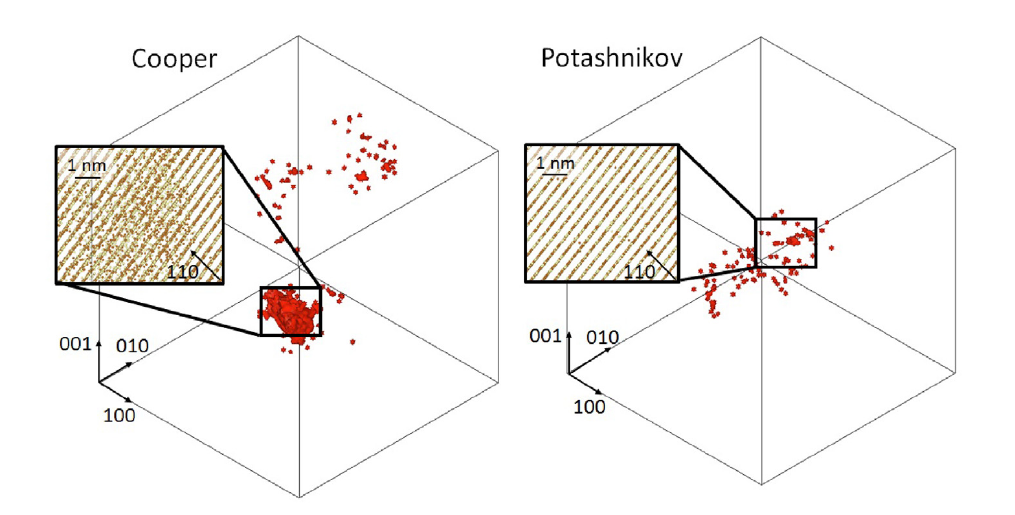
\includegraphics[width=\linewidth]{chapters/interatomic_potential_fitting/images/puo2damage.png}
\caption{Damage in \acrshort{mox} (LAMMPS)\cite{moxlammpsdamage}}
\label{fig:moxlammps}
\endminipage\hfill
\minipage{0.49\textwidth}
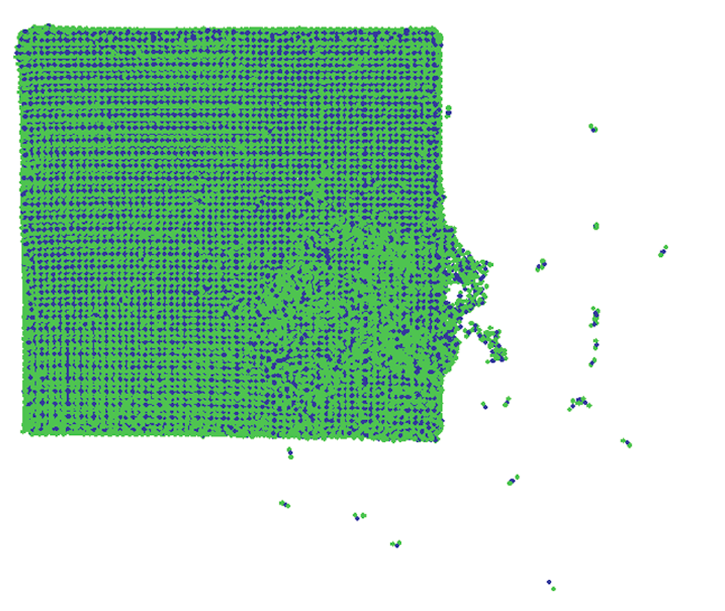
\includegraphics[width=\linewidth]{chapters/interatomic_potential_fitting/images/puo-sputtering.png}
\caption{Sputtering of plutonium oxide (LAMMPS)\cite{pusputtering}}
\label{fig:pusputter}
\endminipage
\end{figure}
\FloatBarrier

Damage cascades in \acrlong{mox}s have been modelled recently using the \acrshort{lammps} code.  A 70x70x70 box with sides approximately 40nm in length and containing 4,116,000 atoms was used with \acrshort{pka}s having energies ranging from 5 to 75keV\cite{moxlammpsdamage} (fig. \ref{fig:moxlammps}).  The sputtering of material from the surface of plutonium oxide (IV) has also been modelled with \acrshort{lammps} using a box of 393,216 atoms with a \acrshort{pka} of 87.7keV\cite{pusputtering} (fig. \ref{fig:pusputter}).  The timescale of the sputtering simulation was 7.8 picoseconds ($7.8 \times 10^{-12}$) and the entire event was split into $1.0 \times 10^{5}$ time steps of $7.8 \times 10^{-17}$s.

\FloatBarrier
\begin{figure}[!htb]
\minipage{0.49\textwidth}
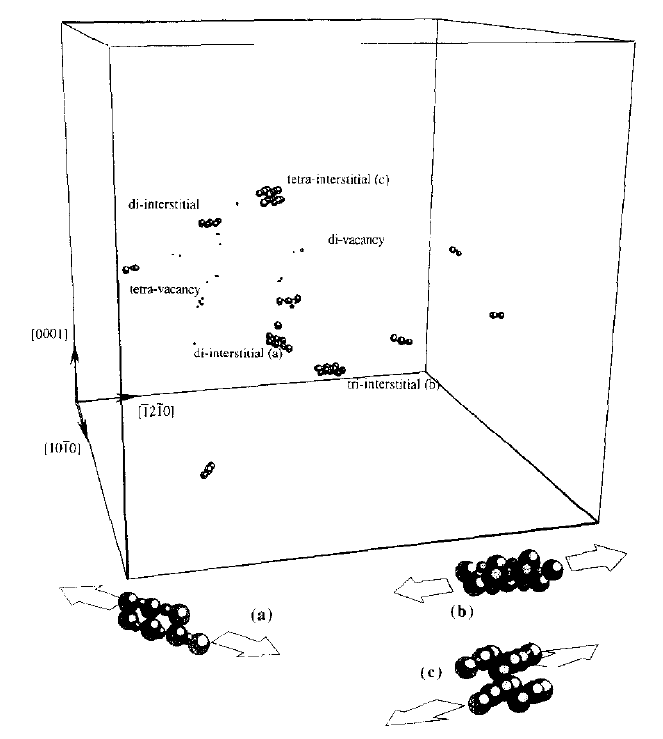
\includegraphics[width=\linewidth]{chapters/interatomic_potential_fitting/images/moldy1.png}
\caption{5keV cascade (MOLDY)\cite{pkamoldy}}
\label{fig:moldy5kev}
\endminipage\hfill
\minipage{0.49\textwidth}
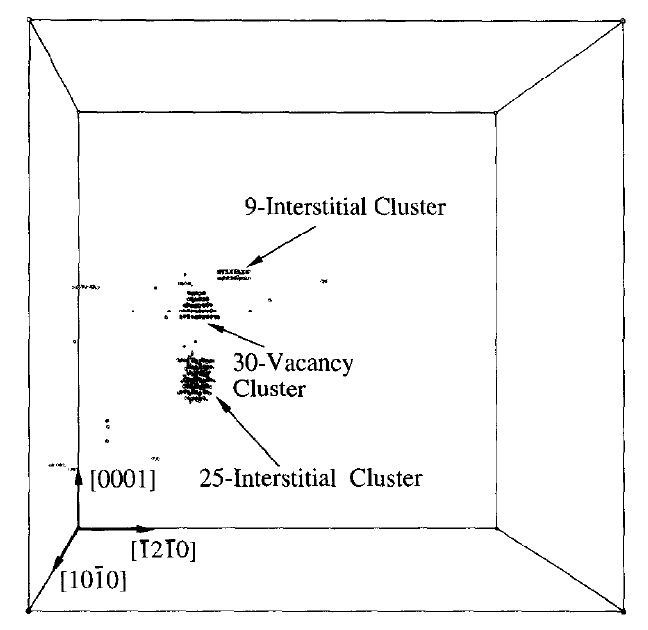
\includegraphics[width=\linewidth]{chapters/interatomic_potential_fitting/images/moldy2.png}
\caption{20keV cascade (MOLDY)\cite{pkamoldy}}
\label{fig:moldy20kev}
\endminipage
\end{figure}
\FloatBarrier

MOLDY has previously been used to model primary knock on atoms in metals, at energies of 5kev, 10keV and 20keV which would be slightly lower than the typical iron \acrshort{pka}s close to U235 fuel in the reactor (fig. \ref{fig:neutronironrecoil}).  This simulation however was in alpha-zirconium and the higher mass of zirconium, relative to iron, would lead to lower energy \acrshort{pka}s.  The damage cascades were modelled in a 104,832 atom block for the 5keV \acrshort{pka} (fig. \ref{fig:moldy5kev}) and a 445,536 atom block for the 20keV \acrshort{pka} (fig. \ref{fig:moldy20kev}).


\FloatBarrier
\begin{figure}[!htb]
\minipage{0.24\textwidth}
\endminipage
\minipage{0.49\textwidth}
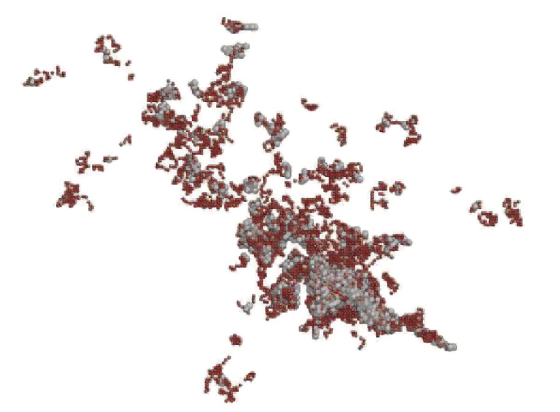
\includegraphics[width=\linewidth]{chapters/interatomic_potential_fitting/images/dlpolycascade.png}
\caption{100keV cascade after 50ps in TiO2 (DL\_POLY)\cite{dlpolyradiationdamage}}
\label{fig:dlpoly100kev}
\endminipage\hfill
\minipage{0.24\textwidth}
\endminipage
\end{figure}
\FloatBarrier

DL\_POLY has also been used to model damage cascades in various oxides (titanium, aluminium, silicon)\cite{dlpolyradiationdamage}.  The \acrshort{pka} energies are higher than those performed in MOLDY 15 years earlier, but still under 1MeV.  The authors expect 1MeV simulation boxes to require at least 1 billion atoms, but the 100-200keV \acrshort{pka}s they modelled were within 10 million atom simulation boxes.  Slightly larger boxes and damage cascades required longer simulation times, and with a box size of 43nm per side, a 50ps simulation time was used (fig. \ref{fig:dlpoly100kev}).

\acrshort{md} codes compute the energy, forces and stress of a collection of atoms in similar ways, although code optimizations may vary.  An overview of the methods used, and replicated in the code created for this work, are discussed in appendix \ref{chap:appendix-activity-v2}.




\subsection{Velocity Verlet Algorithm}

Verlet integration is used by \acrshort{md} codes such as DL\_POLY, \acrshort{lammps}, Democritus as well as \acrshort{md} \acrshort{dft} codes, as in the case of CASTEP.  

First, the forces at time step n are calculated $\vec{f_{n}}$.  Now, using these forces and the velocity at time step n, the half step velocity is computed (eq. \ref{eq:verlet1}).

\begin{equation}
\begin{split}
\vec{v_{n+half}} = \vec{v_{n}} + \frac{\vec{f_{n}} \delta t}{2 m}
\end{split}
\label{eq:verlet1}
\end{equation}

The position of the next step, n + 1, is calculated using the position at n, the time step $dt$ and the half step velocity (eq. \ref{eq:verlet2}).

\begin{equation}
\begin{split}
\vec{r_{n+1}} = \vec{r_{n}} + \vec{v_{n+half}} \times \delta t
\end{split}
\label{eq:verlet2}
\end{equation}

The forces are recalculated at the new position $\vec{r_{n+1}}$ to give $\vec{f_{n+1}}$ and this, along with the half step velocity, is used to compute the velocity at step n+1, $\vec{v_{n+1}}$ (eq. \ref{eq:verlet3}). 

\begin{equation}
\begin{split}
\vec{v_{n+1}} = \vec{v_{n+half}} + \frac{\vec{f_{n+1}} \delta t}{2 m}
\end{split}
\label{eq:verlet3}
\end{equation}

This process is repeated for each time step $\delta t$ from the start of the simulation to the end.  







%%%%%%%%%%%%%%%%%%%%%%%%%%%%%%%%%%%%%%%%%%%%%%%%%%%%%%%%%%%%%%%%%%%%%%%%%%%%%%%%%%%%%%%%%%%%%%%%%%%%%%%%%%
%%
%%  FITTING PROGRAMS
%%
%%%%%%%%%%%%%%%%%%%%%%%%%%%%%%%%%%%%%%%%%%%%%%%%%%%%%%%%%%%%%%%%%%%%%%%%%%%%%%%%%%%%%%%%%%%%%%%%%%%%%%%%%%


\section{Existing Potential Fitting Programs}
\label{section:fittingprograms}

\subsubsection{Bonny Quadratic Program Fitting}

This code has been used to fit a number of potentials, including Fe-Cr and W-Re.  It is a Fortran code and uses known properties of the material in different configurations.  The only functional forms available in the 2012 version of the code are cubic spline for the pair and density functions and a polynomial for the embedding functional.  The fitting subroutine uses quadratic programming to find parameters for the pair and embedding function splines.


\subsubsection{Hepburn FitPot}

FitPot was created by Hepburn, a co-author of papers with Ackland\cite{hepburnfec}.  It was written in Java and tackles the fitting as a non-linear least squares problem.  The \acrfull{lma} is used to minimise the response function and uses the derivatives of the response function with respect to the input parameters to construct the Jacobian that is then used to construct an estimation of the Hessian.


\subsubsection{Brommer PotFit}

Originally developed in C, the PotFit\cite{pbrommer} program uses the force matching method of fitting.  In the early versions of the code, splines were the only function choice available.  In the years since, the option to fit analytic functions has been added.  Simulated annealing is the primary search algorithm that attempts to locate the global minima.  Powell's conjugate direction method is used to locate the local minima once the probable global minima is located.  In order to use PotFit, a database of force, energy and stress for various configurations is required.


\subsubsection{Sheng Modified PotFit}
\label{section:shengeampotentials}

A set of potentials have been derived by Sheng et al\cite{shengeam} and are available to download in tabulated form\cite{shengeamonline}.   They were created using a modified version of the PotFit code by P. Brommer and F. G\"ahler\cite{pbrommer}.  The code had been modified extensively to include quintic spline interpolation, phonon calculation, elastic constant calculation and optimization techniques\cite{shengeamonline}.  The potentials (typically) used 15 knot splines for pair and density functions and 6 knot splines for the embedding functional for each element, but the potentials were published as tabulated functions.  Potentials for fourteen FCC metals were derived in the first instance, but more (including alloys) are available on the website.  Unfortunately, the (Sheng et al.) modified PotFit code is not available through the PotFit website\cite{pbrommer}, and the latest version of their code has moved on since 2011.


\subsubsection{General Utility Lattice Program}
\label{section:gulp}

\acrfull{gulp}\cite{gulp} is a Fortran 90 code that has been developed by Julian Gale since the late 90s.  It is currently in its 6th version and is a large code at over 750,000 lines of code.  It is able to compute many properties of a material and is able to minimise the energy of a system and fit potentials.  Early in this work, \acrshort{gulp} was considered as a possible tool to wrap a potential fitting code around, but without an \acrshort{api} the first approach relied on writing input files and reading output files, which was inefficient.

The author notes in Chapter 1 of the \acrshort{gulp} manual that it is a large code.  Adding the desired forms of potential for radiation damage that included splines and a \acrshort{zbl} core pair potential would have required knowledge of the code and a lot of time to program.  Adding new types of potential such as the \acrshort{2beam} would have resulted in the same issue.


%%%%%%%%%%%%%%%%%%%%%%%%%%%%%%%%%%%%%%%%%%%%%%%%%%%%%%%%%%%%%%%%%%%%%%%%%%%%%%%%%%%%%%%%%%%%%%%%%%%%%%%%%%
%%
%%  DFT
%%
%%%%%%%%%%%%%%%%%%%%%%%%%%%%%%%%%%%%%%%%%%%%%%%%%%%%%%%%%%%%%%%%%%%%%%%%%%%%%%%%%%%%%%%%%%%%%%%%%%%%%%%%%%





\section{Density Functional Theory}
\label{section:dftbackground}

\Acrfull{dft} is a branch of quantum chemistry that approximately solves the Schr\"{o}dinger equation using electron density, rather than the coordinates of each electron in the system.  A number of simplifications are also applied in order for \acrshort{dft} to be practical to use (fig. \ref{fig:dftapproximations}), but despite this calculations are limited to just hundreds or thousands of atoms.  A calculation of a hundred or so atoms may take thousands of \acrshort{cpu} hours at the time of writing, depending on the type of calculation and complexity of the electron structures of the atoms involved.

It is through \acrshort{dft} that the first principles energy, stress and force calculations will be made, and it is these results that the \acrshort{eam} potentials will be trained and fit to using the force matching method.  This will allow much larger scale modelling using the extrapolated behaviour of accurate \acrshort{dft} calculations.



\FloatBarrier
\subsection{Motivation For Using \acrshort{dft} In This Work}

The use of interatomic potentials bridges the gap between the quantum scale and macroscopic scale.  In order to develop these potentials either measurements or calculated values are needed for forces, energies and stresses.  \acrshort{dft} is a convenient choice and has been used to fit potentials and calculate crystal properties many times (Sheng et al\cite{shengeam}, Mehl et al.\cite{mehlsp} Connetable and Thomes,\cite{orthonisi} Ravindran et al\cite{dftrfkj}, Hepburn and Ackland\cite{hepburnfec} and more).


\FloatBarrier
\subsection{Brief Overview of DFT}

Several important theories and approximations are used by \acrshort{dft} with the aim of calculating and minimising energies and forces.  The Born-Oppenheimer approximation separates the electron-nucleus wave function.  It treats the nuclei as fixed points, and the system of electrons in a fixed potential created by the nuclei.


The \acrshort{dft} of Kohn, Sham and Hohenburg proved that the potential of a system is uniquely determined by its ground state density.  This makes solving the Schr\"{o}dinger equation significantly easier.

\begin{figure}[!h]
\centering
\resizebox{0.4\textwidth}{!}{%
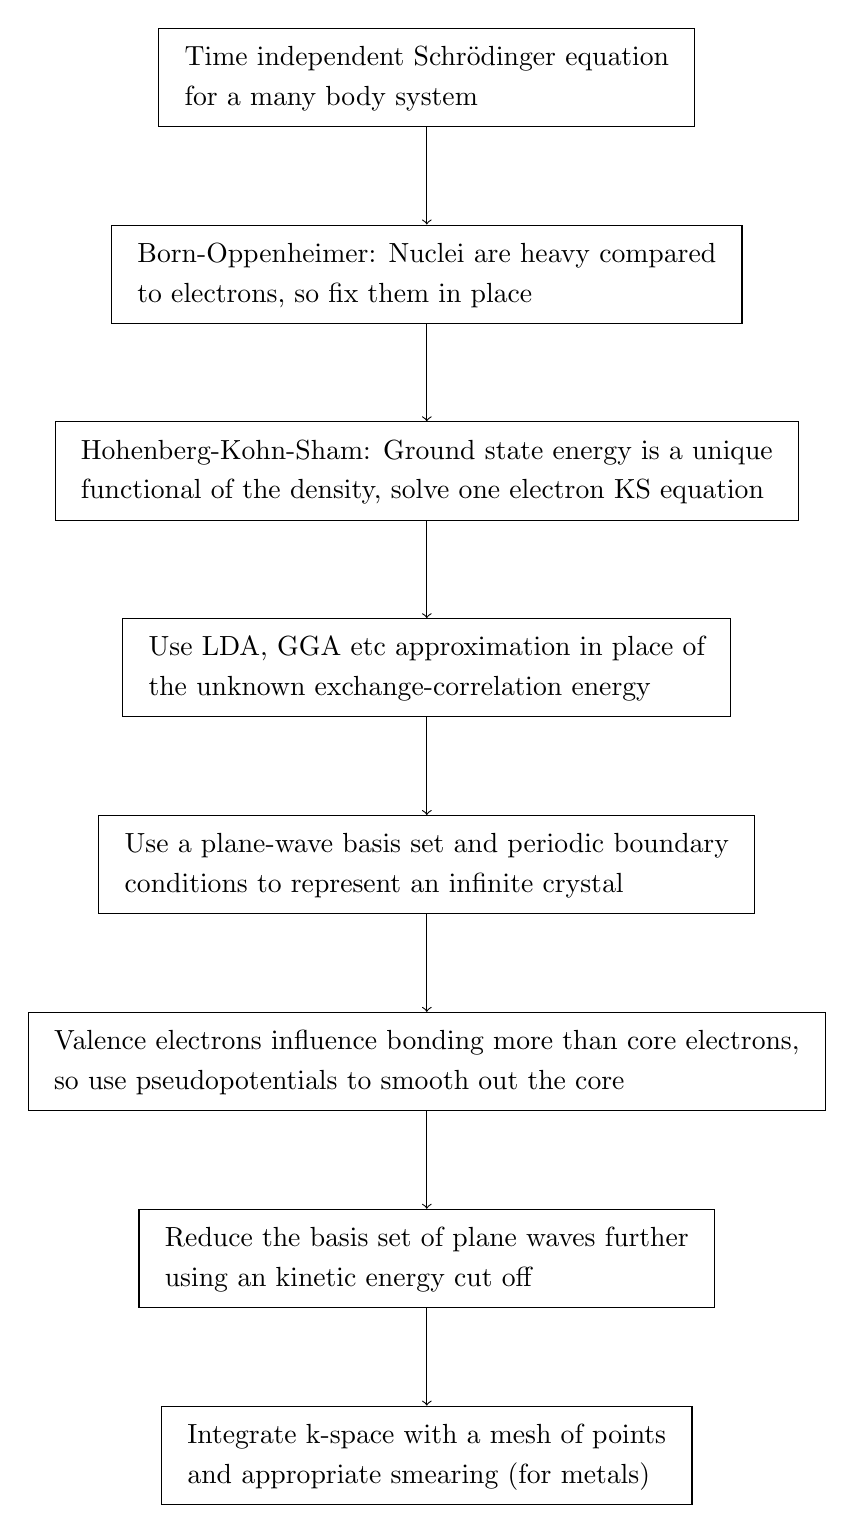
\begin{tikzpicture}[node distance=2.5cm]
\node (a) [rectangle, draw, fill=none] {\begin{tabular}{l}
Time independent Schr\"{o}dinger equation \\
for a many body system
\end{tabular}};
\node (b) [rectangle, draw, fill=none, below of=a] {\begin{tabular}{l}
Born-Oppenheimer: Nuclei are heavy compared \\
to electrons, so fix them in place
\end{tabular}};
\node (c) [rectangle, draw, fill=none, below of=b] {\begin{tabular}{l}
Hohenberg-Kohn-Sham: Ground state energy is a unique \\
functional of the density, solve one electron KS equation
\end{tabular}};
\node (d) [rectangle, draw, fill=none, below of=c] {\begin{tabular}{l}
Use LDA, GGA etc approximation in place of \\
the unknown exchange-correlation energy
\end{tabular}};
\node (e) [rectangle, draw, fill=none, below of=d] {\begin{tabular}{l}
Use a plane-wave basis set and periodic boundary \\
conditions to represent an infinite crystal
\end{tabular}};
\node (f) [rectangle, draw, fill=none, below of=e] {\begin{tabular}{l}
Valence electrons influence bonding more than core electrons, \\
so use pseudopotentials to smooth out the core
\end{tabular}};
\node (g) [rectangle, draw, fill=none, below of=f] {\begin{tabular}{l}
Reduce the basis set of plane waves further \\
using an kinetic energy cut off
\end{tabular}};
\node (h) [rectangle, draw, fill=none, below of=g] {\begin{tabular}{l}
Integrate k-space with a mesh of points \\
and appropriate smearing (for metals)
\end{tabular}};
%% arrows
\draw [->] (a) -- (b);
\draw [->] (b) -- (c);
\draw [->] (c) -- (d);
\draw [->] (d) -- (e);
\draw [->] (e) -- (f);
\draw [->] (f) -- (g);
\draw [->] (g) -- (h);
\end{tikzpicture}
}%
\caption{Common approximations used to enable \acrshort{dft} calculations}
\label{fig:dftapproximations}
\end{figure}








\FloatBarrier
\subsection{\acrlong{tise}}

The Schr\"{o}dinger equation is a linear partial differential wave equation and it was proposed by Erwin Schr\"{o}dinger in 1925.  There is a time-dependent and time-independent form of the equation.  As the \acrshort{dft} calculations in this work are static only the time-independent version will be discussed.  

\begin{equation}
\begin{split}
\hat{H} \lvert \Psi \rangle = E \lvert \Psi \rangle
\end{split}
\label{eq:eqTimeIndependentSchrodinger}
\end{equation}

The \Gls{hamiltonian} $\hat{H}$ is an operator and it is the total energy in the system.  $\Psi$ is the \gls{wavefunction} and this contains all the measurable information possible about whatever it represents.  E is the energy eigenvalue of this system and this will depend on the eigenstate of the system.  The wave function is also connected to the probability of a particle being found at a certain point in space, and the integral over all space is equal to 1 i.e. the probability of it being found somewhere in space is equal to 1 (eq. \ref{eq:foundsomewhere}).

\begin{equation}
\begin{split}
\int_{-\infty}^{\infty} \int_{-\infty}^{\infty}  \int_{-\infty}^{\infty}  \abs{\Psi(x,y,z)}^2 dx dy dz = 1
\end{split}
\label{eq:foundsomewhere}
\end{equation}

The Schr\"{o}dinger equation is set up depending on the system being studied.  Starting with the simplest, a free particle, the only non zero energy of the Hamiltonian is kinetic.


\begin{equation}
\begin{split}
\hat{H} = -\frac{\hbar^2}{2 m} \nabla^2 \\
-\frac{\hbar^2}{2 m} \nabla^2 \Psi(\vec{r}) = E \Psi(\vec{r})
\end{split}
\label{eq:eqTimeIndependentSchrodinger1}
\end{equation}

If the particle is in a potential, it will have both kinetic energy $\hat{T}$ and potential energy $\hat{V}$ (eq. \ref{eq:eqTimeIndependentSchrodinger2}).

\begin{equation}
\begin{split}
\hat{H} = \hat{T} + \hat{V} = -\frac{\hbar^2}{2 m} \nabla^2 + V(\vec{r})\\
\left[-\frac{\hbar^2}{2 m} \nabla^2 + V(\vec{r}) \right] \Psi(\vec{r}) = E \Psi(\vec{r})
\end{split}
\label{eq:eqTimeIndependentSchrodinger2}
\end{equation}




\subsection{Many Body \acrshort{tise}}

Electronic structure calculations are important and allow the calculation of material properties that may be difficult or impossible to measure with current technology.  The next step towards this is to set up the Schr\"{o}dinger equation (time-independent) for nuclei and electrons in a crystal.  

The only potential considered is that due to the electromagnetic force.  The energy operators required are kinetic and electromagnetic potential (eq. \ref{eq:eqTimeIndependentSchrodinger3}).

\begin{equation}
\begin{split}
\hat{H} = \hat{T_e} + \hat{T_n} + \hat{V_{e-e}} + \hat{V_{e-n}} + \hat{V_{n-n}}
\end{split}
\label{eq:eqTimeIndependentSchrodinger3}
\end{equation}

The first two terms are the kinetic energy of the electrons and nuclei respectively (eq. \ref{eq:eqTimeIndependentSchrodinger4}).

\begin{equation}
\begin{split}
\hat{T_e} = - \sum_{i} \frac{\hbar^2}{2 m}  \nabla^2 \text{  sum of kinetic energy of electrons} \\
\hat{T_n} = - \sum_{k} \frac{\hbar^2}{2 M}  \nabla^2 \text{  sum of kinetic energy of nuclei}
\end{split}
\label{eq:eqTimeIndependentSchrodinger4}
\end{equation}

The last three terms are potential energy terms due to the electromagnetic force (eq. \ref{eq:eqTimeIndependentSchrodinger5}). 

\begin{equation}
\begin{split}
V_{e-e} = \frac{1}{2} \sum_{i,j,i \neq j} \frac{1}{\abs{\vec{r}_i - \vec{r}_j}} \text{  sum of potential energy between electrons} \\
V_{e-n} = \sum_{i,k} \frac{z_i}{\abs{\vec{r}_i - \vec{r}_l}} \text{  sum of potential energy between electrons and nuclei} \\
V_{n-n} = \frac{1}{2} \sum_{k,l,k \neq l} \frac{z_k z_l}{\abs{\vec{r}_l - \vec{r}_k}} \text{  sum of potential energy between nuclei}
\end{split}
\label{eq:eqTimeIndependentSchrodinger5}
\end{equation}

These operators are now input into the \acrshort{tise} (eq. \ref{eq:eqTimeIndependentSchrodinger6}).


\begin{equation}
\begin{split}
\left[ \left(- \sum_{i} \frac{\hbar^2}{2 m} - \sum_{k} \frac{\hbar^2}{2 M} \right) \nabla^2  + \sum_{i,k} \frac{z_i}{\abs{\vec{r}_i - \vec{r}_l}} + \frac{1}{2} \left( \sum_{i,j,i \neq j} \frac{1}{\abs{\vec{r}_i - \vec{r}_j}} + \sum_{k,l,k \neq l} \frac{z_k z_l}{\abs{\vec{r}_l - \vec{r}_k}} \right) \right] \lvert \Psi \rangle = E \lvert \Psi \rangle
\end{split}
\label{eq:eqTimeIndependentSchrodinger6}
\end{equation}



\subsection{Born-Oppenheimer}

The \acrshort{tise} arrived at is far too complicated to solve, even for the simple ensembles of atoms.  It represents the many body system of electrons and nuclei, and it takes the positions of all nuclei and electrons as input variables (eq. \ref{eq:eqTimeIndependentSchrodinger7}).

\begin{equation}
\begin{split}
\hat{H} \lvert \Psi (\vec{r_e}, \vec{r_n}) \rangle = E \lvert \Psi (\vec{r_e}, \vec{r_n}) \rangle \\
\text{ where } \vec{r_e} = r_{e,1}, r_{e,1},...,r_{e,i} \text{ (electron positions)} \\
\text{ where } \vec{r_n} = r_{n,1}, r_{n,1},...,r_{n,i} \text{ (electron positions)} \\
\end{split}
\label{eq:eqTimeIndependentSchrodinger7}
\end{equation}

In 1927 the Born-Oppenheimer approximation was proposed to separate the electron components from the nuclei in the Hamiltonian.  Protons and neutrons are almost 2,000 times the mass of electrons.  With respect to the electrons, they move much slower and may be considered to be fixed or frozen in place.  Simplifying for a moment to a single electron and proton, due to Newton's second law, we can see that the acceleration of the electron would be similarly 2,000 times that of the proton: $f_e = f_p$ and $m_e a_e = m_p a_p$ which leads to $a_e = \frac{m_p}{m_e} a_p$.  As the nuclei move, the electrons are assumed to respond instantly, remaining in the ground state and not being promoted into higher energy levels.

The Hamiltonian for the electrons may be written with the electron co-ordinates as a variable, and the nuclei co-ordinates as a parameter (eq. \ref{eq:eqTimeIndependentSchrodinger8}).

\begin{equation}
\begin{split}
\hat{H_e} (\vec{r_e}; \vec{r_n}) = \hat{T_e}(\vec{r_e}) + \hat{V_{e-e}}(\vec{r_e}) + \hat{V_e-n}(\vec{r_e}; \vec{r_n})
\end{split}
\label{eq:eqTimeIndependentSchrodinger8}
\end{equation}

The wavefunction and energy for the electrons may be calculated, although if the nuclear cooridinates are changed, i.e. by changing the parameter $r_n$, the wavefucntion and energy will need to be recalculated.

\begin{equation}
\begin{split}
\hat{H_e} (\vec{r_e}; \vec{r_n}) \psi_{e} (\vec{r_e}; \vec{r_n}) = E_e (\vec{r_n})  \psi_{e} (\vec{r_e}; \vec{r_n}) 
\end{split}
\label{eq:elechamiltonian}
\end{equation}


\begin{equation}
\begin{split}
\Psi (\vec{r_e}, \vec{r_n}) = \chi_{ne} (\vec{r_e}) \psi_{e} (\vec{r_e}; \vec{r_n})
\end{split}
\label{eq:combinedwavefunction}
\end{equation}

The electronic Hamiltonian (eq. \ref{eq:elechamiltonian}) is still dependent on the electronic co-ordinates.  As there are three co-ordinates per electron, there are 3 dimensions when solving for a hydrogen atom.  For an Iron atom, with 26 electrons, there are 78 dimensions, and for a 4x4x4 FCC supercell of Iron there would be 256 atoms, 26 electrons per atom and 3 dimensions per electon, giving a total of 19,968 dimensions.  Even for small numbers of electrons, solving this equation is impractical.




\subsection{Crystals, Reciprocal Space and Bloch Theorem}
\label{section:crystalsrecipbloch}

A Bravais lattice is a construct used to describe a periodic crystal lattice.  It has the following properties given in eq. \ref{eq:reciprocalspace}. 

\begin{equation}
  \begin{split}
    \vec{R} = n_1 \vec{a}_1 + n_2 \vec{a}_2 + n_3 \vec{a}_3 \\
    n_1 , n_2, n_3 \in Z \\
    \vec{a}_1, \vec{a}_2, \vec{a}_3 \text{ are independent}
  \end{split}
  \label{eq:reciprocalspace}
\end{equation}

There are 14 Bravais lattices and 7 families of these lattices, and these lattices may be grouped by vector length and angle relationships (table. \ref{table:bravaisvectors}).  This work is primarily concerned with cubic and tetragonal crystals, although distortions are applied to these crystals throughout.

\begin{table}[h]
\begin{center}
\renewcommand{\arraystretch}{1.2}
\begin{tabular}{c c c}
\hline\hline
Class & Lengths & Angles \\
\hline\hline
Cubic & $a = b = c$ & $ \alpha = \beta = \gamma = 90 $ \\
Hexagonal & $a = b, c $ & $ \alpha = \beta, \gamma = 120 $ \\
Rhombohedral & $a = b = c $ & $ \alpha = \beta = \gamma \neq 90 $ \\
Tetragonal & $a = b, c $ & $ \alpha = \beta = \gamma = 90 $ \\
Orthorhombic & $a, b, c $ & $ \alpha = \beta = \gamma = 90 $ \\
Monoclinic & $a, b, c $ & $ \alpha = \beta = 90, \gamma \neq 90 $ \\
Triclinic & $a, b, c $ & $ \alpha, \beta, \gamma, $ \\
\hline
\end{tabular}
\caption{Bravais lattice vector length and angle relationships}
\label{table:bravaisvectors}
\end{center}
\end{table}



\subsubsection{Bloch Theorem}
\label{section:blochtheorem}

Metals are made up from grains which in turn are crystal lattices of atoms.  Despite the majority of metals being composed of a large collection of microscopic crystals, rather than being a single perfect crystal, most of their properties may be calculated as if the metal were a single crystal.

The grain size of water quenched SS304 is approximately 30 micrometers across\cite{grainsizesteel}.  If the crystal were a cube, it would contain $2.0 \times 10^{15}$ atoms and it would have sides over 100,000 atoms in length.

In solid state physics, in order to solve the \acrshort{tise} for such a system, it is useful to consider an infinite sized crystal.  It may be helpful to visualise this as a \enquote{ring} of atoms in one dimension (fig. \ref{image:1dchainofatoms}) or as a super-cell with periodic boundary conditions in three dimensions.


\begin{figure}[htbp]
\begin{center}
\begin{minipage}{.47\textwidth}
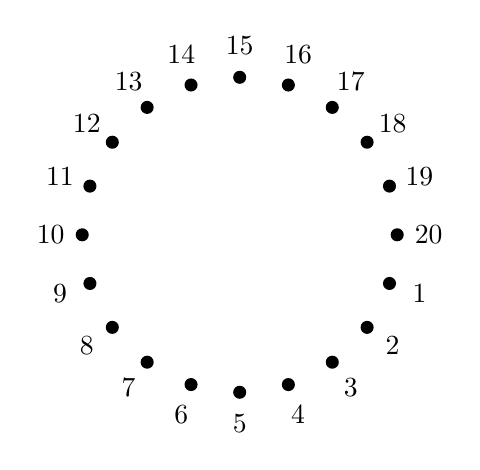
\begin{tikzpicture}
    % equidistant points and arc
    \foreach \x [count=\p] in {0,...,19} {
        \node[shape=circle,fill=black, scale=0.5] (\p) at (-\x*18:2) {};};
    \foreach \x [count=\p] in {1,...,20} {
        \draw (-\x*18:2.4) node {\p};}; 
\end{tikzpicture}
\caption{A useful, albeit incorrect, way of visualising an "infinite" chain of atoms in 1D}
\label{image:1dchainofatoms}
\end{minipage}
\begin{minipage}{.05\textwidth}
\end{minipage}
\begin{minipage}{.47\textwidth}

\begin{tikzpicture}
\tikzdrawline{col_000000}{0}{0}{0}{1}{0}{6}
\tikzdrawline{col_000000}{2}{0}{0}{3}{0}{6}
\tikzdrawline{col_000000}{4}{0}{0}{5}{0}{6}
\tikzdrawline{col_000000}{6}{0}{0}{7}{0}{6}
\tikzdrawline{col_000000}{8}{0}{0}{9}{0}{6}
\tikzdrawline{col_000000}{0}{0}{0}{8}{0}{0}
\tikzdrawline{col_000000}{0.333333}{0}{2}{8.33333}{0}{2}
\tikzdrawline{col_000000}{0.6666}{0}{4}{8.66666}{0}{4}
\tikzdrawline{col_000000}{1}{0}{6}{9}{0}{6}

\tikzdrawlinedotted{col_000000}{1.0}{0}{6}{1.1}{0}{6.5}
\tikzdrawlinedotted{col_000000}{3.0}{0}{6}{3.1}{0}{6.5}
\tikzdrawlinedotted{col_000000}{5.0}{0}{6}{5.1}{0}{6.5}
\tikzdrawlinedotted{col_000000}{7.0}{0}{6}{7.1}{0}{6.5}
\tikzdrawlinedotted{col_000000}{9.0}{0}{6}{9.1}{0}{6.5}

\tikzdrawlinedotted{col_000000}{-0.1}{0}{-0.5}{0.0}{0}{0}
\tikzdrawlinedotted{col_000000}{1.9}{0}{-0.5}{2}{0}{0}
\tikzdrawlinedotted{col_000000}{3.9}{0}{-0.5}{4}{0}{0}
\tikzdrawlinedotted{col_000000}{5.9}{0}{-0.5}{6}{0}{0}
\tikzdrawlinedotted{col_000000}{7.9}{0}{-0.5}{8}{0}{0}

\tikzdrawlinedotted{col_000000}{-0.5}{0}{0}{0.0}{0}{0}
\tikzdrawlinedotted{col_000000}{-0.22222}{0}{2}{0.3333}{0}{2}
\tikzdrawlinedotted{col_000000}{0.11111}{0}{4}{0.6666}{0}{4}
\tikzdrawlinedotted{col_000000}{0.5}{0}{6}{1.0}{0}{6}

\tikzdrawlinedotted{col_000000}{8}{0}{0}{8.5}{0}{0}
\tikzdrawlinedotted{col_000000}{8.3333}{0}{2}{8.83333}{0}{2}
\tikzdrawlinedotted{col_000000}{8.6666}{0}{4}{9.1666}{0}{4}
\tikzdrawlinedotted{col_000000}{9.0}{0}{6}{9.5}{0}{6}

\tikzdrawlinethick{col_000000}{0}{0}{0}{0.333}{0}{2}
\tikzdrawlinethick{col_000000}{2}{0}{0}{2.333}{0}{2}
\tikzdrawlinethick{col_000000}{0}{0}{0}{2}{0}{0}
\tikzdrawlinethick{col_000000}{0.3333}{0}{2}{2.333}{0}{2}

\tikzdrawlinethick{col_000000}{4.3333}{0}{2}{4.6666}{0}{4}
\tikzdrawlinethick{col_000000}{6.3333}{0}{2}{6.6666}{0}{4}
\tikzdrawlinethick{col_000000}{4.3333}{0}{2}{6.3333}{0}{2}
\tikzdrawlinethick{col_000000}{4.6666}{0}{4}{6.6666}{0}{4}

\tikzdrawline{col_000000}{1.1}{0}{2}{1.33333}{0}{3}
\tikzdrawarrow{col_000000}{1.33333}{0}{3}{4.45}{0}{3}{above}{$\vec{R}$}

\node[] at (1.1,1.0) {$\vec{r}$};
\node[] at (5.5,3.0) {$\vec{r} + \vec{R_{t}}$};
\end{tikzpicture}
\caption{A 2D example of a translation by an integer multiple of the unit cell from the origin unit cell}
\label{image:2dtranslation}

\end{minipage}
\end{center}
\end{figure}




\FloatBarrier
As the structure is a repeating lattice, any point within a unit cell is equivalent to any other point translated by an integer multiple of the lattice vector (fig. \ref{image:2dtranslation}).

\begin{equation}
  \begin{split}
    \psi(\vec{r}) = \psi(\vec{r} + \vec{R_t}) \\
    \text{where } \vec{R_t} = n_1 \vec{R}_{1} + n_2 \vec{R}_{2} + n_3 \vec{R}_{3} \\
    \text{where } \vec{R} \text{ is the real lattice vector}
  \end{split}
  \label{eq:eqEulersFormula}
\end{equation}


Reciprocal space, also known as k-space or momentum space, is a mathematical construct.  It is an imaginary space where the lengths, and volumes, are the inverse of real space and planes of atoms are represented as points. 

%\begin{figure}[htbp]
%\begin{center}
%\begin{minipage}{.4\textwidth}
%\begin{tikzpicture}
%\tikzcoordgrid{4.0}{4.0}{4.0}{$\vec{a_1}$}{$\vec{a_1}$}{$\vec{a_1}$}
%\end{tikzpicture}
%\end{minipage}
%\begin{minipage}{.1\textwidth}
%\end{minipage}
%\begin{minipage}{.4\textwidth}
%\begin{tikzpicture}
%\tikzcoordgrid{4.0}{4.0}{4.0}{$\vec{b_1}$}{$\vec{b_1}$}{$\vec{b_1}$}
%\end{tikzpicture}
%\end{minipage}
%\caption{Graph caption}
%\label{graph:graph1}
%\end{center}
%\end{figure}

Starting with a lattice of points in real space $\vec{R}$, points in reciprocal space $\vec{G}$ only are valid points if $\exp(i \vec{G} \cdot \vec{R}) = 1$\cite{solidstatebasics}.  A real space vector $\vec{R}$ is transformed to it's reciprocal in the following way, where $\Omega$ is the volume of the primitive cell in real space.

\begin{equation}
  \begin{split}
    \vec{g_1} = \frac{2 \pi}{\Omega} \vec{r_2} \times \vec{r_3} \\
    \vec{g_2} = \frac{2 \pi}{\Omega} \vec{r_3} \times \vec{r_1} \\
    \vec{g_3} = \frac{2 \pi}{\Omega} \vec{r_1} \times \vec{r_2} \\
    \Omega = \vec{r_1} \cdot (\vec{r_2} \times \vec{r_3}) \\
  \end{split}
  \label{eq:eqReciprocalLattice}
\end{equation}

If the crystal structure is modelled as an infinitely repeating lattice, the potential also has the same periodicity (eq. \ref{eq:eqReciprocalLattice}).

\begin{equation}
  \begin{split}
    V(\vec{r}) = V(\vec{r} + \vec{R}_{t}) 
  \end{split}
  \label{eq:eqPeriodicPotential1}
\end{equation}

As the potential is a periodic function, it may be written as a fourier series in reciprocal space (eq. \ref{eq:eqPeriodicPotentialSeries1}).

\begin{equation}
  \begin{split}
    V(\vec{r}) = \sum_{\vec{G}} V_{\vec{G}} \exp(i \vec{G} \cdot \vec{r})
  \end{split}
  \label{eq:eqPeriodicPotentialSeries1}
\end{equation}

The wave function for an electron ($\psi_{n\vec{k}}$) in the lattice is assumed periodic with the lattice structure (eq. \ref{eq:eqPeriodicWavefunction}) and may be written as the product of a \gls{planewave} and a cell periodic function ($u_{n\vec{k}}$), where $n$ denotes the band and $\vec{k}$ is the wave vector.

\begin{equation}
  \begin{split}
    u_{n\vec{k}}(\vec{r}) = u_{n\vec{k}}(\vec{r} + \vec{R_{t}})
  \end{split}
  \label{eq:eqPeriodicWavefunction}
\end{equation} 

\begin{equation}
  \begin{split}
    \psi_{n\vec{k}} (\vec{r}) = u_{n\vec{k}}(\vec{r}) \exp(i \vec{k} \cdot \vec{r})\\
    \psi_{n\vec{k}} (\vec{r}) = \psi_{n\vec{k}} (\vec{r}) \exp(i \vec{k} \cdot \vec{R_{t}})
  \end{split}
  \label{eq:eqPeriodicPotentialSeries2}
\end{equation}

The Born-von Karman boundary conditions apply eq. \ref{eq:eqPeriodicWavefunction} and eq. \ref{eq:eqPeriodicPotentialSeries2} to the wave function such that:

\begin{equation}
  \begin{split}
    \psi_{n\vec{k}} (\vec{r} + \vec{R}_{t}) = \psi_{n\vec{k}} (\vec{r}) \
    \text{where  } \vec{R_t} = \sum_i N_i \vec{a_i} \
    \text{and  } N_i \in \mathbb{Z}
  \end{split}
  \label{eq:eqPeriodicPotentialSeries4}
\end{equation}

With these boundary conditions and use of plane waves, \Gls{blochtheorem} replaces an enormous number of electrons with an infinite number electrons in a periodic lattice where only those in the unit cell need to be considered.

\FloatBarrier
\begin{figure}[!htb]
\minipage{0.49\textwidth}
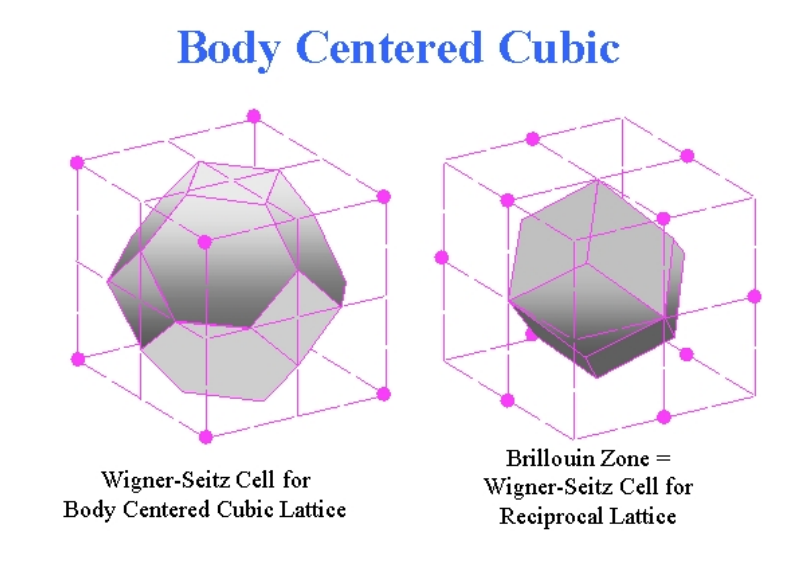
\includegraphics[width=\linewidth]{chapters/interatomic_potential_fitting/images/bcc_wcs_bz.png}
\caption{BCC Wigner Seitz Cell and \acrshort{bz} \cite{fccbccreciprocal}}
\label{fig:bccrecip}
\endminipage\hfill
\minipage{0.49\textwidth}
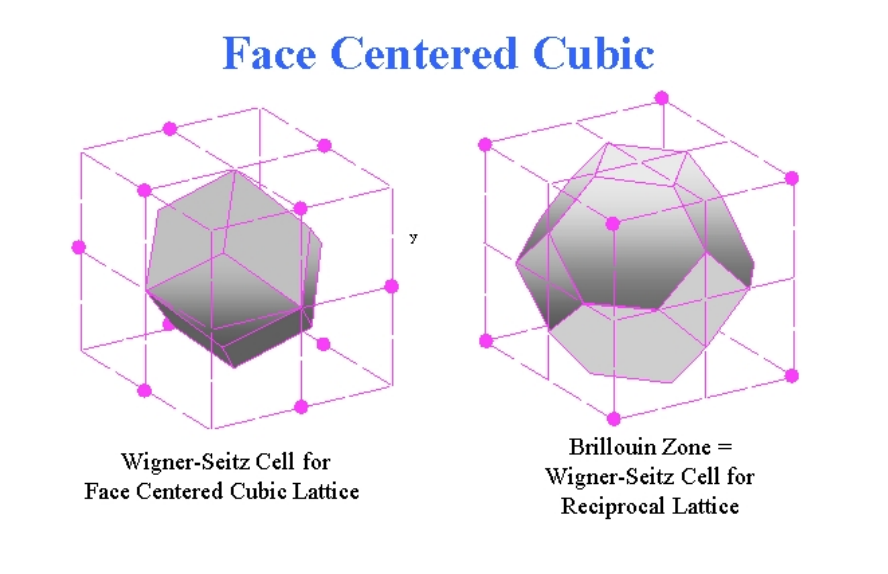
\includegraphics[width=\linewidth]{chapters/interatomic_potential_fitting/images/fcc_wcs_bz.png}
\caption{FCC Wigner Seitz Cell and \acrshort{bz} \cite{fccbccreciprocal}}
\label{fig:fccrecip}
\endminipage
\end{figure}
\FloatBarrier

The (first) \Gls{brillouinzone} is a volume in (3D) reciprocal space and it is analogous to the \Gls{wignerseitzcell} in real space (figs. \ref{fig:bccrecip} and \ref{fig:fccrecip}).  It is the primitive lattice cell in reciprocal space.  The reciprocal of a \acrshort{bcc} lattice is a \acrshort{fcc} lattice (fig. \ref{fig:bccrecip}) and vice versa (fig. \ref{fig:fccrecip}).  In real space a point anywhere in the lattice is a integer multiple of the lattice vector away from the same point in the origin \Gls{wignerseitzcell}.  There are an infinite number of wave vectors $\vec{k}$ in reciprocal space, but by virtue of the periodicity of the lattice, they are also all found within the Brillouin Zone.  If the crystal has symmetries, the \acrshort{bz} may be reduced further to the \acrlong{ibz}.

Within the \acrshort{bz} there are energy surfaces.  Picking a straight line through reciprocal space allows one to plot the energy bands along that one dimensional space.  A particularly important energy surface is the Fermi surface and, in the one electron model, this marks the boundary between the occupied and unoccupied states at 0K \cite{hjonesfermi}.  The \Gls{fermienergy} is the energy of the highest occupied state at 0K.



\subsection{\Acrlong{hk} Theorem}

In the 1960s, Hohenberg and Kohn\cite{hohenbergkohn} simplified the problem of solving the many electron \acrshort{tise} in an exact way by proving:

\begin{itemize}
\item in an external potential $v(\vec{r})$, the potential is uniquely determined by the density of the ground state $n_0(\vec{r})$ assuming that the particles are non-degenerate
\item a uniquely defined functional $E[\rho(\vec{r})]$ exists and the ground state energy, $min(E[\rho(\vec{r})])$, is found by varying the density
\end{itemize}

The proof starts by picturing a box of electrons that interact with each other through coulomb repulsion within an external potential  $\vec{v}(r)$, for example the potential of \enquote{fixed} nuclei following the Born Oppenheimer approximation.

\begin{equation}
\begin{split}
\hat{H} = \hat{T} + \hat{V} = -\frac{1}{2} \nabla^2 + V(\vec{r}) \\
\left[-\frac{1}{2} \nabla^2 + V(\vec{r}) \right] \Psi(\vec{r})_{0} = E_{0} \Psi(\vec{r})
\end{split}
\label{eq:eqtishk}
\end{equation}

\begin{equation}
\begin{split}
\hat{H} = \hat{T} + \hat{V} + \hat{U}
\end{split}
\label{eq:eqHKhamiltonian}
\end{equation}

where

\begin{equation}
\begin{split}
T = \frac{1}{2} \int \nabla \psi^{*}(\vec{r})\nabla \psi(\vec{r}) d\vec{r}
\end{split}
\label{eq:eqHKKinetic}
\end{equation}

\begin{equation}
\begin{split}
V = \int v(\vec{r}) \psi^{*}(\vec{r}) \psi (\vec{r}) d\vec{r} 
\end{split}
\label{eq:eqHKexternal}
\end{equation}

\begin{equation}
\begin{split}
U = \frac{1}{\lvert \vec{r} - \vec{r}' \rvert} \psi^{*}(\vec{r}) \psi^{*}(\vec{r'}) \psi(\vec{r}) \psi(\vec{r}') d\vec{r} d\vec{r'}
\end{split}
\label{eq:eqHKinteraction}
\end{equation}

In the eqs. \ref{eq:eqHKhamiltonian} \ref{eq:eqHKKinetic} \ref{eq:eqHKhamiltonian} \ref{eq:eqHKinteraction} the hamiltonian operator $\hat{H}$ is a sum of the kinetic energy $\hat{T}$, the mutual coulomb repulsion $\hat{U}$ and the operator due to an external potential (due to the nuclei) $\hat{V}$.  The non degenerate ground state electron density is $n(\vec{r}) = \langle \Phi \lvert \phi^{*}(\vec{r}) \phi(\vec{r}) \rvert \Phi \rangle$.

The \acrshort{hk} theorem shows that the external potential $v(\vec{r})$ is a unique functional of the electron density $n(\vec{r})$.  The proof is that by contradiction where by two different states are assumed to have the same ground state charge density.


\minipage{0.49\textwidth}
\centering
\textbf{State A} \\
$\Psi_{A}$ with potential $V_A(\vec{r})$ \\
Hamiltonian $\hat{H} = \hat{T} + \hat{V_A} + \hat{U}$ \\
\acrshort{tise} $\hat{H_A} \Psi_A = E_A \Psi_A$\\
Assumption - this state has the charge density $n(\vec{r})$
\endminipage
\minipage{0.49\textwidth}
\centering
\textbf{State B} \\
$\Psi_{B}$ with potential $V_B(\vec{r})$ \\
Hamiltonian $\hat{H} = \hat{T} + \hat{V_B} + \hat{U}$ \\
\acrshort{tise} $\hat{H_B} \Psi_B = E_B \Psi_B$\\
Assumption - this state has the charge density $n(\vec{r})$
\endminipage

The minimal property of the ground state gives the following\cite{hohenbergkohn}\cite{hohenbergkohnleeuwen}:

\begin{equation}
\begin{split}
E_A = \langle \Phi_A \lvert \hat{H_A} \rvert \Phi_A \rangle \\
E_A = \langle \Phi_A \lvert \hat{H_B} + \hat{V_A} - \hat{V_B} \rvert \Phi_A \rangle \\
E_A = \langle \Phi_A \lvert \hat{H_B} \rvert \Phi_A \rangle + \int d^3 \vec{r} n(\vec{r})(v_A(\vec{r}) - v_B(\vec{r})) \\
\end{split}
\label{eq:minimalproperty}
\end{equation}

\begin{equation}
\begin{split}
E_A > E_B + \int d^3 \vec{r} n(\vec{r})(v_A(\vec{r}) - v_B(\vec{r}))
\end{split}
\label{eq:minimalproperty1}
\end{equation}

The indices A and B are interchanged to give a second equation:

\begin{equation}
\begin{split}
E_B > E_A + \int d^3 \vec{r} n(\vec{r})(v_B(\vec{r}) - v_A(\vec{r})) \\
E_B > E_A - \int d^3 \vec{r} n(\vec{r})(v_A(\vec{r}) + v_B(\vec{r}))
\end{split}
\label{eq:minimalproperty2}
\end{equation}

By adding eq. \ref{eq:minimalproperty1} and eq. \ref{eq:minimalproperty2} together the integrals will cancel out.

\begin{equation}
\begin{split}
E_A + E_B > E_A + E_B
\end{split}
\label{eq:hkcontradiction}
\end{equation}

This (eq. \ref{eq:hkcontradiction}) is a contradiction and proves the first part of the \acrshort{hk} theorem: $v(\vec{r})$ is uniquely determined by $n(\vec{r})$.  If the charge density is known, a single external potential exists for it.

%\FloatBarrier
%\begin{figure}[!htb]
%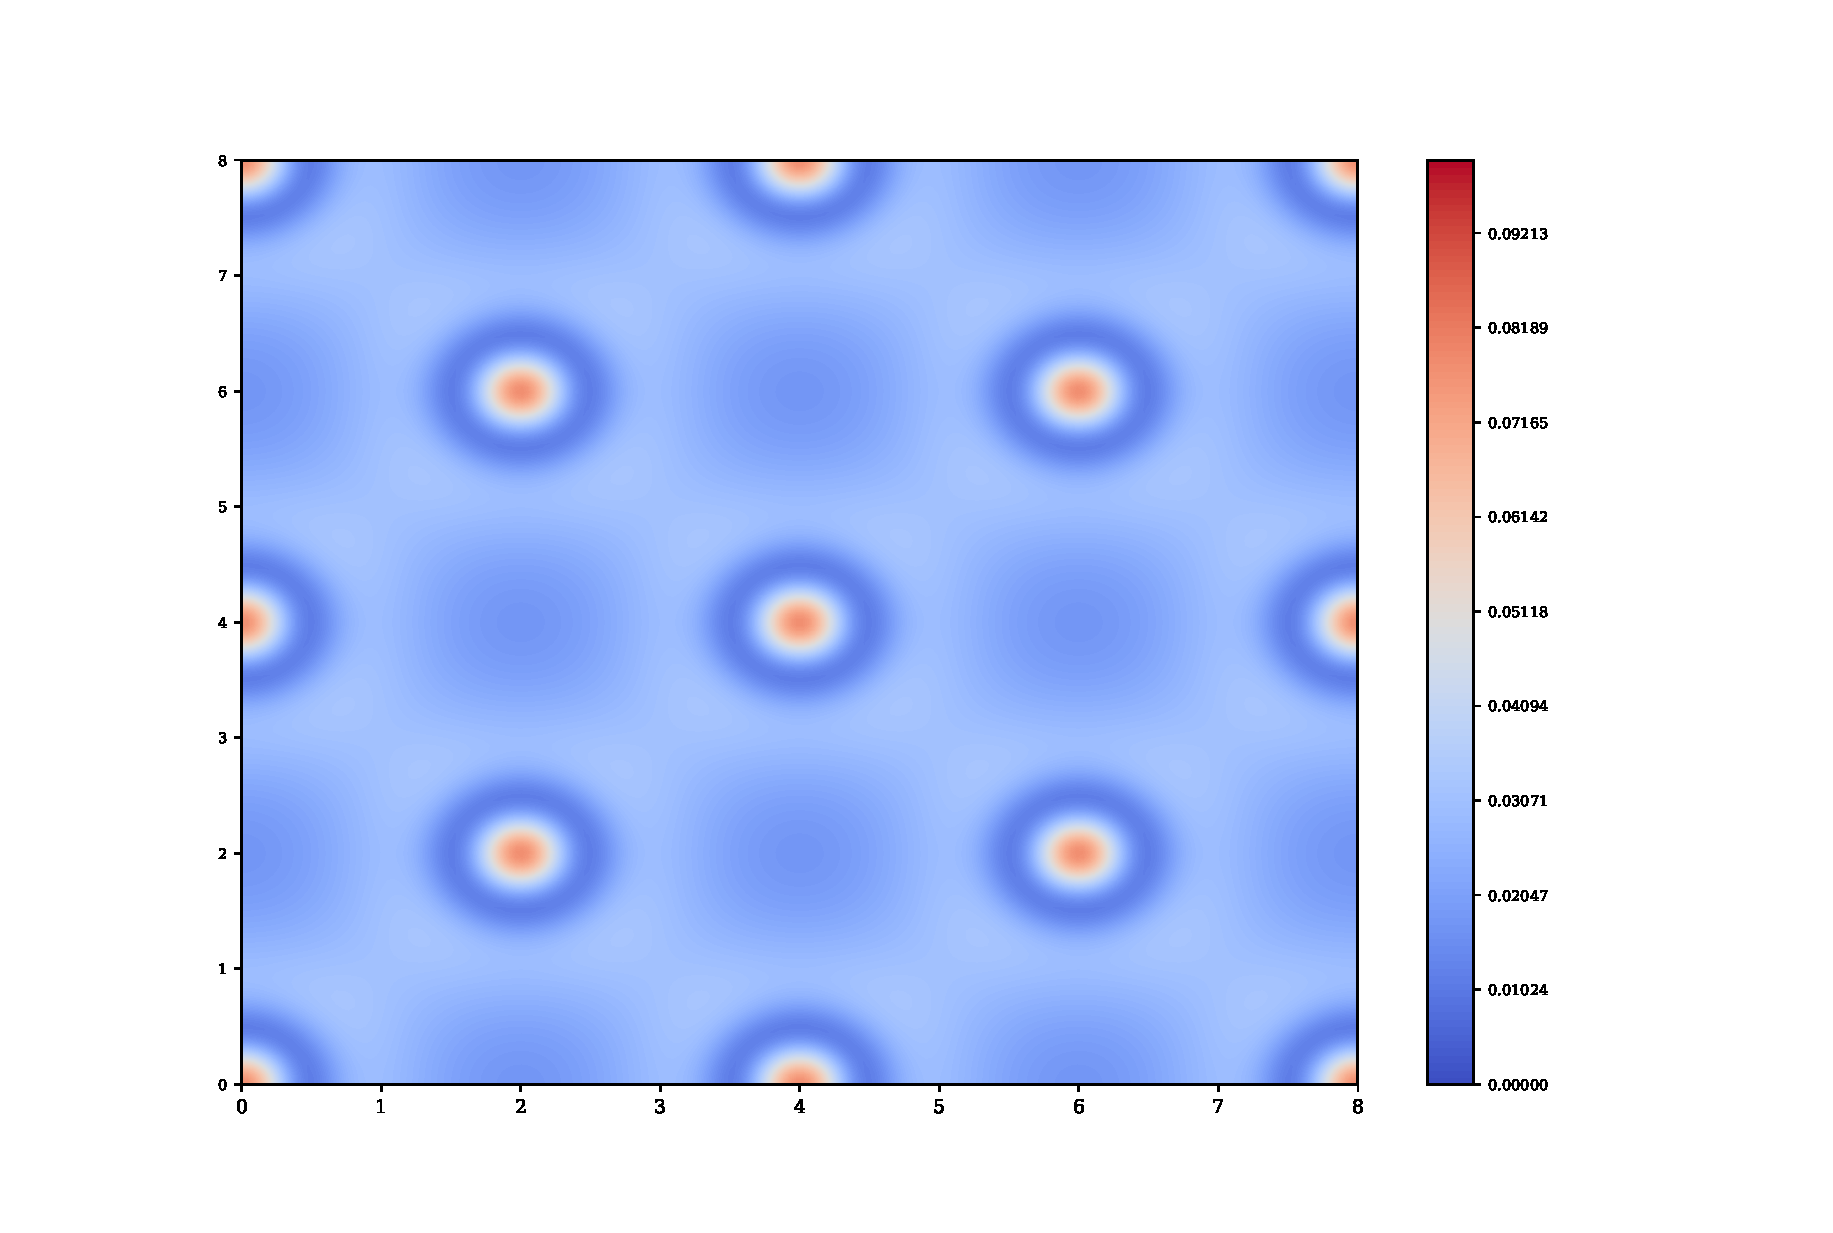
\includegraphics[width=0.8\linewidth]{chapters/interatomic_potential_fitting/images/layer0000.eps}
%\caption{Charge density FCC aluminium xy plane at $z=0.0 a_0$}
%\label{fig:cdalfcc1}
%\end{figure}

%\begin{figure}[!htb]
%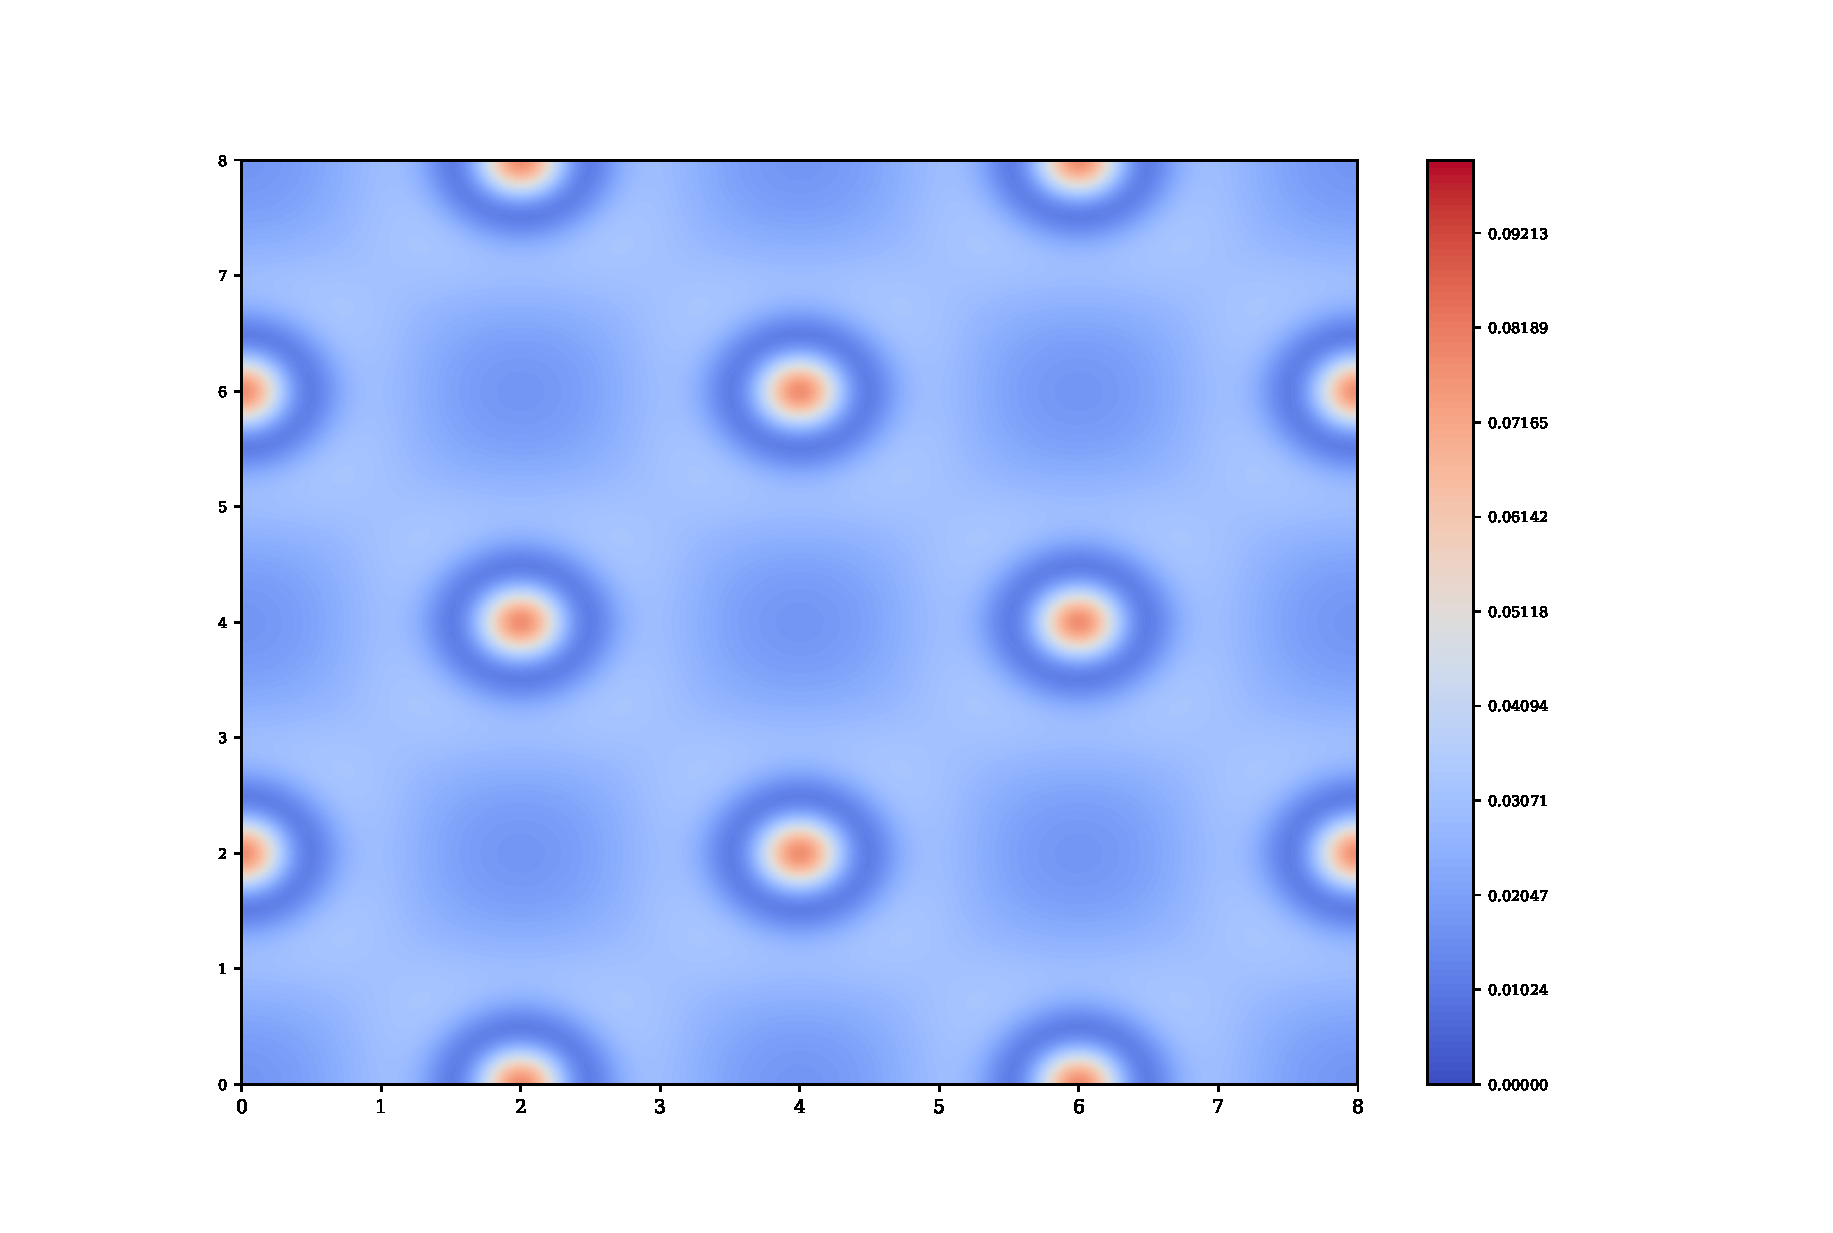
\includegraphics[width=0.8\linewidth]{chapters/interatomic_potential_fitting/images/layer0050.eps}
%\caption{Charge density FCC aluminium xy plane at $z=0.5 a_0$}
%\label{fig:cdalfcc2}
%\end{figure}


The next part of the theorem is to show that the energy functional $E[n(\vec{r})]$ exists and the minimum can be found by varying the charge density function.  The kinetic and interaction functional $\hat{T}$ and $\hat{U}$ define a functional $F[n(\vec{r})]$.

\begin{equation}
\begin{split}
F[n(\vec{r})] \equiv \langle \Phi \lvert \hat{T} + \hat{U} \rvert \Phi \rangle 
\end{split}
\label{eq:hkffunctional}
\end{equation}

This is a universal functional\cite{hohenbergkohn} and it makes up a part of the energy functional.  The energy functional is comprised of the \acrshort{hk} functional $F[n(\vec{r})]$ and the external potential as shown in eq. \ref{eq:hkefunctional}.

\begin{equation}
\begin{split}
E[n(\vec{r})] \equiv \int v(\vec{r}) n(\vec{r}) d\vec{r} + F[n]
\end{split}
\label{eq:hkefunctional}
\end{equation}

For the ground state electron density $n(\vec{r})$ the energy will be equal to the ground state energy $E_0 = E_v[n]$.  Where N is the number of particles in the system, the integral of the density over all space will sum to N (eq. \ref{eq:nint}).

\begin{equation}
\begin{split}
N[n] = \int n(\vec{r}) d\vec{r}
\end{split}
\label{eq:nint}
\end{equation}

If the system has N particles the energy level for a none ground state energy, k, is given in eq. \ref{eq:groundstateenergy}.

\begin{equation}
\begin{split}
\epsilon_{v,k} [\Psi_k] \equiv \langle \Phi_k \lvert \hat{V} \rvert \Phi_k \rangle - \langle \Phi_k \lvert \hat{T} - \hat{U} \rvert \Phi_k \rangle 
\end{split}
\label{eq:groundstateenergy}
\end{equation}

This has a minimum where $\Psi_k = \Psi_0$, the ground state.

\begin{equation}
\begin{split}
\epsilon_{v,k} [\Psi_k] = \int v(\vec{r}) n_k(\vec{r}) d\vec{r} + F[n_k] \\
\epsilon_{v,0} [\Psi_k] = \int v(\vec{r}) n_0(\vec{r}) d\vec{r} + F[n_0] \\
\epsilon_{v,k} > \epsilon_{v,0}
\end{split}
\label{eq:groundstateenergy1}
\end{equation}

\begin{comment}
###############################
Variational method shows that, given a system $\hat{H} \lvert \Psi_n \rangle = E_n \lvert \Psi_n \rangle$, the expectation value of $\hat{H}$ for an arbitrary state $\lvert \Psi_a \rangle$ must satisfy:

\begin{equation}
\begin{split}
\hat{H} \Psi_{n} = E_{n} \Psi_{n}
\end{split}
\label{eq:eqVariationalMethod1}
\end{equation}

Next, take the inner product (eq. \ref{eq:eqVariationalMethod2}) then rearrange the equation (eq. \ref{eq:eqVariationalMethod3}).

\begin{equation}
\begin{split}
\expval{\hat{H}}{\Psi_{n}} = E_{n} \bra{\Psi}\ket{\Psi}
\end{split}
\label{eq:eqVariationalMethod2}
\end{equation}

\begin{equation}
\begin{split}
\langle \hat{H} \rangle = \frac{\expval{\hat{H}}{\Psi_{n}}}{\bra{\Psi}\ket{\Psi}} \geq E_{n}
\end{split}
\label{eq:eqVariationalMethod3}
\end{equation}

Minimise to find the ground state energy.

Now assume that a second, different, external potential exists with the ground state $\Psi'$ and the same density $n(\vec{r})$.  $\Psi \neq \Psi'$

As a result of the Hohenberg-Kohn theorem, we are able to calculate the electronic energy of a system from the charge density.
###############################
\end{comment}




\subsection{Kohn-Sham Equations}

The year following the Hohenberg-Kohn theorem, a set of self-consistent equations were derived by Kohn and Sham.  The ground state energy of \underline{interacting} \gls{jellium} in the potential of fixed nuclei, an external potential, can be written as follows\cite{kohnsham}: 

\begin{equation}
E = T_{s} + U + V_{n-e} + E_{xc}
\end{equation}

\begin{equation}
E = T_{s}[\rho(\vec{r})] + \int d \vec{r} v(\vec{r}) \rho(\vec{r}) + \frac{1}{2} \int \int  d \vec{r} d \vec{r'} \frac{\rho(\vec{r}) \rho(\vec{r'}) }{\lvert \vec{r} - \vec{r'} \rvert} + E_{xc}[\rho(\vec{r})]
\end{equation}

The kinetic energy, $T_s$, is that of a system of \underline{non interacting} particles and $E_{xc}$ is the exchange and correlation of an \underline{interacting system}.  The exchange and correlation energy functional exists, but is unknown.  

The \Gls{kohnshameq} are used to calculate the energy of a many body Schr\"{o}dinger equation by solving for a single electron.

\begin{equation}
\hat{H}_{KS} \psi_{i} = E_{i} \psi_{i}
\label{eq:eqKS1}
\end{equation}

\begin{equation}
\left(-\frac{1}{2} \nabla^2 + \hat{v}_{KS}[n](\vec{r}) \right) \psi_{i}(\vec{r}) = E_{i} \psi_{i}(\vec{r})
\label{eq:eqKS2}
\end{equation}

\begin{equation}
\begin{split}
\hat{v}_{KS}(\vec{r_e}, \vec{r_n}) = v_{n-e}(\vec{r_e}, \vec{r_n}) + \int d^3\vec{r'} \frac{\rho(\vec{r_{e}'})}{\lvert \vec{r_{e}} - \vec{r_{e}'} \rvert } + v_{xc}[\rho](\vec{r_{e}})
\end{split}
\label{eq:eqGroundState}
\end{equation}

\begin{equation}
n(\vec{r}) = \sum_i^N \lvert \psi_{i}(\vec{r}) \lvert^2
\label{eq:eqKS2b}
\end{equation}



It is important to note that even though this is a one electron equation it is an exact solution.


\subsection{Self-Consistent Solution}
\FloatBarrier

The \Gls{kohnshameq} cannot be solved in the usual way.  They require a value for the density, but the density is obtained by solving the equations, so there is a dilemma.  It can however be solved self consistently: an initial density is guessed, and this is repeatedly updated until the density in and out values are the same (or within a set convergence threshold).  The basic algorithm used by PWscf from the Quantum Espresso suite is shown in fig. \ref{fig:selfconsistentalgorithm}\cite{abcdftsissa}.



\begin{figure}[htb]
\centering
\begin{tikzpicture}

\node (eq-a) [rectangle, draw, align=left] {
Solve $\hat{H_{ks}} \psi_i = e_i \psi_i$ }; 

\node (flow-aa) [rectangle, draw, align=left, below = of eq-a] {
Construct $V_{ks} = V_{ne} + V_{ee}[\rho] + V_{xc}[\rho]$};
 
\node (flow-ba) [rectangle, draw, align=left, below = of flow-aa] {
Guess $\rho_{in}$}; 


\node (flow-ca) [rectangle, draw, align=left, below = of flow-ba] {
Compute $V_{ks}$}; 

\node (flow-da) [rectangle, draw, align=left, below = of flow-ca] {
Diagonalize $H_{ks}$}; 

\node (flow-ea) [rectangle, draw, align=left, below = of flow-da] {
Compute $rho_{out}$}; 

\node (flow-fa) [diamond, node distance=3cm, draw, below of=flow-ea] {$\rho_{in} == \rho_{out}$};
\node (flow-fb) [rectangle, draw, align=left, left = of flow-fa] {
No}; 

\node (flow-fbb) [rectangle, draw, align=left, above = of flow-fb] {
Mix}; 

\node (flow-fc) [rectangle, draw, align=left, right = of flow-fa] {
Yes};

\node (flow-ga) [rectangle, draw, align=left, below = of flow-fc] {
End \\
Compute energy, forces etc};

\path [draw, -latex'] (flow-aa) -- (flow-ba);
\path [draw, -latex'] (flow-ba) -- (flow-ca);
\path [draw, -latex'] (flow-ca) -- (flow-da);
\path [draw, -latex'] (flow-da) -- (flow-ea);
\path [draw, -latex'] (flow-ea) -- (flow-fa);
\path [draw, -latex'] (flow-fa) -- (flow-fb);
\path [draw, -latex'] (flow-fb) -- (flow-fbb);
\path [draw, -latex'] (flow-fbb) |- (flow-ba);
\path [draw, -latex'] (flow-fa) -- (flow-fc);
\path [draw, -latex'] (flow-fc) -- (flow-ga);

\end{tikzpicture}
\caption{\Acrshort{scf} algorithm for Quantum Espresso}
\label{fig:selfconsistentalgorithm}
\end{figure}

In practice the input and output densities may never be exactly the same so rather than wait indefinitely for convergence, a threshold is set.  The smaller the threshold the more iterations and time would be expected to pass, but the calculation will be closer to the solution.

With each iteration the density of the last iteration is mixed into a new density.  If simple linear mixing is used a mixing beta determines the ration of new to old density as given in eq. \ref{eq:linearmixing}\cite{jfannett1996}.

\begin{equation}
\begin{split}
\rho^{n+1} = (1 - \beta) \rho_{KS}^{n} + \beta \rho_{out}^{n}
\end{split}
\label{eq:linearmixing}
\end{equation}

More advanced mixing methods include Newton-Raphson or Broyden mixing.  The PWscf program within Quantum Espresso uses Broyden for charge density mixing by default.  Charge sloshing is an issue where convergence is slow or never happens.  This is a particular problem for metals\cite{chargesloshing2} and is more significant the larger the system\cite{localtf}.  The Thomas-Fermi screening used is based on the work by Johnson\cite{thomasfermijohnson} and this works well for highly homogenous systems.  Further work by Raczkowski, Canning and Wang\cite{localtf} developed a Pulay-Thomas-Fermi method that is implemented in PWscf with the local-TF mixing mode, and this is better suited to highly inhomogeneous systems.

\FloatBarrier
\subsection{Exchange-Correlation Energy}

The \Gls{kohnshameq} have an exchange-correlation energy and this functional is used to collect together the electron energy not captured in the non-interacting energy functionals.

The \Gls{pauliexp} states that two \gls{fermion}s, half integer spin particles, cannot occupy the same quantum state.  This is why electrons occupy a unique orbital within an atom defined by the quantum numbers n, l, $m_l$ and $m_s$.  Consider two particles at points $\vec{r_a}$ and $\vec{r_b}$; the probability amplitude of the wavefunction of these particles equals 1.

\begin{equation}
  \begin{split}
    \lvert \Psi(\vec{r_a}, \vec{r_b}) \rvert ^2 = 1
  \end{split}
  \label{eq:eqEulersFormula}
\end{equation}

Exchanging the particles must also give the same result; they still must exists somewhere with probability 1.

\begin{equation}
  \begin{split}
    \lvert \Psi(\vec{r_b}, \vec{r_a}) \rvert ^2 = 1
  \end{split}
  \label{eq:eqEulersFormula}
\end{equation}

Bosons, integer spin particles, are symmetric when exchanged:

\begin{equation}
  \begin{split}
  \Psi(\vec{r_a}, \vec{r_b}) = \Psi(\vec{r_b}, \vec{r_a})
  \end{split}
  \label{eq:eqEulersFormula}
\end{equation}

Fermions, on the other hand, are antisymmetric:

\begin{equation}
  \begin{split}
  \Psi(\vec{r_a}, \vec{r_b}) = - \Psi(\vec{r_b}, \vec{r_a})
  \end{split}
  \label{eq:eqEulersFormula}
\end{equation}

By setting up a wavefunction for two Fermions, and exchanging them, it can be seen why they cannot exist in the same state.

\begin{equation}
  \begin{split}
  \Psi_{ab} =  \psi_{1}(\vec{r_a}, \vec{r_b}) - \psi_{2}(\vec{r_b}, \vec{r_a})
  \end{split}
  \label{eq:eqEulersFormula}
\end{equation}

\begin{equation}
  \begin{split}
  \Psi_{ab} =  \psi_{1}(\vec{r_a}, \vec{r_b}) - \psi_{2}(\vec{r_a}, \vec{r_b}) = 0
  \end{split}
  \label{eq:eqEulersFormula}
\end{equation}

The \acrshort{xc} term combines the difference between the real system and the fictitious non-interacting system set out in the Kohn-Sham equations.  It also includes the difference between the quantum mechanical electron-electron repulsion and classical electron-electron repulsion.  Unfortunately, whilst we know a functional exists, we do not know the exact form of it\cite{ldaggaperdew}.


 
\subsection{Pseudopotentials}
\label{section:backgroundpseudopotentials}

Plane wave basis sets are used to help solve the \acrshort{tise}.  The \acrshort{dft} code used in this work is Quantum Espresso, and the binary that carries out the calculations is named PWscf: plane wave self consistent field. 

Where $\vec{G}$ is the reciprocal lattice vector, a summation of plane waves may be used to construct each electronic wave function (eq. \ref{eq:waveFunctionPlaneWave})\cite{paynedftreview}.

\begin{equation}
  \begin{split}
  \Psi_{\vec{k}, n} = \sum_{\vec{G}}^{\lvert \vec{G} \rvert < \vec{G_{max}}} c_{\vec{k} + \vec{G}, n} \exp(i(\vec{k} + \vec{G}) \dot \vec{r})
  \end{split}
  \label{eq:waveFunctionPlaneWave}
\end{equation}

Unfortunately, the plane-wave basis sets required are too large to be used in practice, as the would need to represent the tight, rapidly oscillating inner orbitals as well as the \gls{valenceelectron}s.

Bonding and material properties are primarily determined by valence electrons, not core electrons.  Iron, for example, has two valence electrons in the 4s shell; however, it is a transition metal and the partially empty 3d shell is also important to consider.  The core electrons do not contribute as much to the bond and the model may be simplified using pseudopotentials.

\begin{figure}[!htbp]
  \begin{center}
    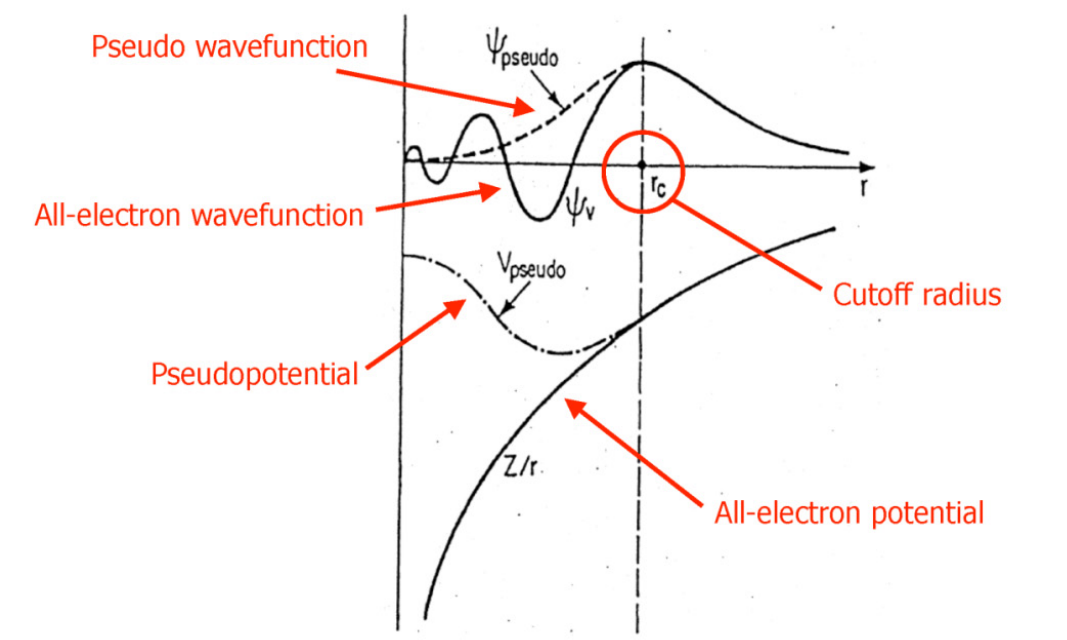
\includegraphics[width=.4\linewidth]{chapters/interatomic_potential_fitting/images/pp.png}
    \caption{Replacing the complex potentials with a pseudopotential\cite{ppselloni}}
    \label{fig:pseudopotentials}
  \end{center}
\end{figure}

The eigen-energies of core electrons are also much larger than properties we see in materials, such as the cohesive energies and this also raises a concern that including the core electrons may introduce errors that are on a similar scale to the energies we are calculating.

The rapidly oscillating function in the core is replaced by a smoother pseudopotential (fig. \ref{fig:pseudopotentials}).  The same material properties are calculated as the valence electron functions are preferenced, but a much small basis set is required to do so.  There are a wide range of pseudopotentials available to use in DFT calculations, and one major distinguishing feature is how they treat the \acrshort{xc} potential $v_{xc} ([n]; \vec{r})$.  

\begin{equation}
\begin{split}
\left(\frac{1}{2} + V_{ext}(\vec{r}) + V_{H}(\vec{r}) + V_{xc}(\vec{r})\right) \psi_{k,\sigma}(\vec{r}) = \epsilon_{k, \sigma} \psi_{k,\sigma}(\vec{r})
\end{split}
\label{eq:Fermi-Dirac distribution}
\end{equation}

The \acrshort{ks} equation consists of several potentials including the \acrfull{xc} energy.  This term represents the many-electron effects. 

\subsubsection{\acrshort{lda}}

The \acrlong{lda} replaces the electron density with \gls{jellium}, a \gls{heg}.  Kohn and Sham, in their original 1965 work, introduced jellium as the density model and, despite its simplicity in comparison to the real electron density distribution, it has worked well for simple metals.

The \acrshort{xc} energy for the \acrshort{lda} is an integral over space in the local neighbourhood of the point of interest.  Both the exchange term ($e_x$) and correlation term ($e_c$) are functionals of the local electron density ($\rho(\vec{r})$).

\begin{equation}
\begin{split}
E_{xc}^{LDA}[\rho] = \int d^3\vec{r} \rho(\vec{r})[e_x (\rho(\vec{r})) + e_c (\rho(\vec{r}))
\end{split}
\label{eq:lda}
\end{equation}

Several different \acrshort{lda} functionals have been developed over the years, including that of Perdew and Zunger.  This functional takes the form given in eq. \ref{eq:perdewzunger}\cite{dftgupta1}.

\begin{equation}
\begin{split}
\epsilon_{C} [n(\vec{r})] = \left\{ \begin{matrix} \frac{-0.14231}{1+1.9529 r_s^{(0.5)} + 0.334 r_s}  & r_s >= 1  \\ -0.0480+0.0311 \ln(r_s) - 0.0116 r_s + 0.0020 r_s \ln(r_s)  & r_s < 1 \end{matrix} \right . 
\end{split}
\label{eq:perdewzunger}
\end{equation}

\subsubsection{\acrshort{lsda}}

Electrons are fermions and have half integer spin.  When trapped in a potential, such as an atom or a crystal lattice, electrons must take difference quantum states and one of the parameters is the spin of the electron.  The \acrshort{lda} does not treat spin at all, but the \acrshort{lsda} splits the density into spin up ($\rho_{\uparrow}$) and down spin ($\rho_{\downarrow}$) (eq. \ref{eq:lsdaDensity}\cite{ldaggaperdew}).

\begin{equation}
\begin{split}
\rho_{\uparrow}(\vec{r}) = \sum_{k}^{occ} \lvert \phi_{k, \uparrow}(\vec{r})\rvert^2 \\
\rho_{\downarrow}(\vec{r}) = \sum_{k}^{occ} \lvert \phi_{k, \downarrow}(\vec{r})\rvert^2 \\
\rho(\vec{r}) = \rho_{\uparrow}(\vec{r}) + \rho_{\downarrow}(\vec{r}) \\
\end{split}
\label{eq:lsdaDensity}
\end{equation}

As with the \acrshort{lda} the exchange and correlation terms are separate but the \acrshort{xc} energy is now dependent on the spin up and spin down density as well as the position (eq. \ref{eq:lsdaXcEnergy}\cite{ldaggaperdew}), where $\zeta(\vec{r})$ is the relative spin-polarisation.  Setting this to 0 reverts this to the spin unpolarised case.

\begin{equation}
\begin{split}
E_{xc}^{LSDA}[\rho_{\uparrow},\rho_{\downarrow}] = \int d^3\vec{r} \rho(\vec{r})[e_x (\rho(\vec{r})) f(\zeta(\vec{r})) + e_c (\rho(\vec{r}), \zeta(\vec{r}))] \\
\zeta = \frac{\rho_{\uparrow} - \rho_{\downarrow}}{\rho_{\uparrow} + \rho_{\downarrow}} \\
 f(\zeta) = \frac{1}{2} \left((1 + \zeta)^{4/3} + (1 - \zeta)^{4/3}\right)
\end{split}
\label{eq:lsdaXcEnergy}
\end{equation}

The energy of the system now being solved is also dependent upon the charge density and spin polarization (eq. \ref{eq:sdftEnergy}).

\begin{equation}
\begin{split}
E = T[\rho, \zeta] + E_{ext} [\rho] + \frac{1}{2} E_{ee}[\rho] + E_{xc}[\rho, \zeta]
\end{split}
\label{eq:sdftEnergy}
\end{equation}

Many correlation energy functionals have been developed in order to improved the \acrshort{lsda} and it is still widely used as will be discussed in section \ref{section:ggavslsda}.  There are now more complicated approaches including the \acrshort{gga}. 


\subsubsection{\acrshort{gga}}

In the \acrshort{lda} and \acrshort{lsda} approximations, the electron density is that of an homogeneous electron gas that does not represent the real electron density.  The density of this gas may change in space, but locally it is a constant density with no gradient.

\begin{equation}
\begin{split}
E_{xc}^{GGA} [\rho_{\uparrow}, \rho{\downarrow}] = \int d^3r f(\rho_{\uparrow}, \rho{\downarrow}, \nabla \rho_{\uparrow}, \nabla \rho{\downarrow})
\end{split}
\label{eq:ggaexchangecorrelation}
\end{equation}

The GGA functional (eq. \ref{eq:ggaexchangecorrelation} \cite{ldaggaperdew}) takes the spin up ($\rho_{\uparrow}$) spin down($\rho_{\downarrow}$) electron densities as well as the gradients of the spin densities ($\nabla \rho_{\uparrow}, \nabla \rho{\downarrow}$).  

The \acrshort{pbe} functional was developed to address some of the short falls of the Perdew-Wang PW91 \acrshort{lsda} functional.  These include an over complication in the formulation of PW91 and that it was designed to satisfy many exact conditions.  The \acrshort{pbe} development focused more on energetically significant conditions\cite{perdewggamadesimple}.

\begin{equation}
\begin{split}
E_{c}^{PBE} [\rho_{\uparrow}, \rho{\downarrow}] = \int d^3r \rho[e_c (r_s, \zeta) + H(r_s, \zeta, t)] 
\end{split}
\label{eq:pbecorrelation}
\end{equation}

\begin{equation}
\begin{split}
E_{x}^{PBE} [\rho] = \int d^3r \rho e_x(\rho) F_x(s)
\end{split}
\label{eq:pbeexchange}
\end{equation}

The functional is split into a correlation energy (eq. \ref{eq:pbecorrelation}) and exchange energy (eq. \ref{eq:pbeexchange}).  $\zeta$ is the relative spin polarization $\zeta = (\rho_{\uparrow}-\rho_{\downarrow})/(\rho_{\uparrow} + \rho_{\downarrow})$ and $r_s$ is the local Seitz radius where $\rho = 3/4 \pi r_s^3$.  The functions $e_x(\rho)$ and $e_c(\rho)$ are the exchange and correlation energy per electron of unpolarised uniform electron gas\cite{ldaggaperdew}.  

Both functionals $H(r_s, \zeta, t)$ and $F_x(s)$ are dependent upon $t$ and $s$ and these in turn are dependent upon the density and density gradients.  Derived by Perdew, Burke and Ernzerhof\cite{perdewggamadesimple}, there is a full description outlined in a later review by Ziesche, Kurth and Perdew\cite{ldaggaperdew}.  A full description of the functional and the terms is also included in appendix \ref{chaper:pbefunctional}.


\subsubsection{\acrshort{lsda} vs \acrshort{gga} Potentials}
\label{section:ggavslsda}

Typically, \acrshort{gga} is an improvement over \acrshort{lsda}, with improvements in the total energies and structural energy differences\cite{perdewggamadesimple}.  Another short coming of \acrshort{lsda} is that it predicts FCC to be the optimal structure for pure iron at 0K, which is incorrect\cite{perdewggabackwardforward}.  A list of success stories and failures were discussed shortly after the publication of the \acrshort{pbe} functional and these are summarised in fig. \ref{fig:pbesuccessfailure}\cite{ldaggaperdew}.

\begin{figure}
\begin{minipage}[t]{.42\textwidth}
Successes of GGA
\begin{itemize}
\item atomization energy of molecules better
\item binding energy curves more realistic
\item Fe is bcc ferromagnetic with GGA (fcc non-magnetic with LSDA)
\item Gives the anti \gls{invareffect} in gamma-Fe and fc Fe-Mn 
\item Improvement on 4\% accuracy for \acrshort{lsda} of alkali metal lattice constants
\item Better lattice constants and bulk moduli of transition metals
\item Isostructural transformation from open to close packed improved
\item Successful calculation of a monovacancy in silicon
\item Oxidation of the Si(001) surface using spin polarized \acrshort{gga}
\end{itemize}
\end{minipage}
\begin{minipage}{.15\textwidth}
\end{minipage}
\begin{minipage}[t]{.42\textwidth}
Failures
\begin{itemize}
\item exchange-correlation holes can be unrealistic under some circumstances
\item works better for exchange correlation together than either alone
\item interaction of electrons in different shells poorly described
\end{itemize}
\end{minipage}
\caption{Successes and failures of the \acrshort{gga} functional\cite{ldaggaperdew}}
\label{fig:pbesuccessfailure}
\end{figure}

\begin{table}[h]
\begin{center}
\renewcommand{\arraystretch}{1.2}
\begin{tabular}{c c c c}
\hline\hline
Parameter & Experimental & LDA & GGA  \\
\hline\hline
a/angs & 8.27 & 8.08 & 8.21 \\
b/angs & 4.80 & 4.74 & 4.81 \\
c/angs & 8.55 & 8.53 & 8.64 \\
$B_0$ (Reuss)/GPa & 146.8 & 156.9 & 141.9 \\
$B_0$ (Voigt)/GPa & 150.9 & 159.1 & 145.0 \\
$C_{11}$/GPa & 317.5 & 377.2 & 326.0 \\
$C_{22}$/GPa & 320.4 & 341.1 & 298.4 \\
$C_{33}$/GPa & 413.2 & 425.3 & 371.9 \\
$C_{44}$/GPa & 112.5 & 136.5 & 123.5 \\
$C_{55}$/GPa & 75.8 & 93.7 & 85.3 \\
$C_{66}$/GPa & 117.5 & 154.6 & 135.9 \\
$C_{12}$/GPa & 29.3 & 27.8 & 22.4 \\
$C_{13}$/GPa & 38.4 & 21.3 & 26.5 \\
$C_{23}$/GPa & 86.0 & 95.1 & 105.5 \\
\hline\hline
\end{tabular}
\end{center}
\caption{Experimental vs \acrshort{lsda} vs \acrshort{gga} for $TiSi_2$\cite{dftrfkj}}
\label{table:ldaggatisi2}
\end{table}

In the literature, investigations into comparisons between \acrshort{gga}, \acrshort{lda} and experiments have been carried out for Titanium Disilicide ($TiSi_2$) and Lanthanum aluminate ($LaAlO_3$).  This work is briefly discussed to highlight the fact that certain pseudopotentials and exchange functionals better reproduce a particular material and property.

In the case of the compound $TiSi_2$, \acrshort{gga} is in better agreement, overall, with experiment than \acrshort{lda}, although several values are better predicted by the latter.  As shown in table \ref{table:ldaggatisi2}, the data shows that \acrshort{lda} is within 1.26\% of the experimental lattice parameters, 6.16\% of the experimental bulk modulus and 18.3\% the value of the experimental elastic constants; several of these were particularly poor, with an almost 45\% disagreement.  On the other hand, \acrshort{gga} is within 0.66\% of the experimental lattice parameters, 3.62\% of the experimental bulk modulus and 14.97\% the value of the experimental elastic constants\cite{dftrfkj}.

$LaAlO_3$ has also been studied using \acrshort{dft}, but this material is better modelled (to reproduce lattice parameters and bulk modulus) with either \acrshort{lda} or a specific form of \acrshort{gga}, the \acrfull{pbesol} potential.  The \acrshort{pbesol} is a revised \acrshort{pbe} functional designed to better reproduce lattice parameters for solids, as shown in table \ref{table:ldaggalaal03}.

\begin{table}[h]
\begin{center}
\renewcommand{\arraystretch}{1.2}
\begin{tabular}{c c c c c}
\hline\hline
Parameter & Experimental & LDA & GGA & GGA (PBESOL) \\
\hline\hline
a/angs & 3.78 & 3.74 & 3.82 & 3.77 \\
$B_0$/GPa & 215 & 224.00 & 190.35 & 206.41 \\
\hline\hline
\end{tabular}
\end{center}
\caption{Experimental vs \acrshort{lsda} vs \acrshort{gga} vs \acrshort{gga} PBESOL for $LaAlO_3$\cite{laalo3gga}}
\label{table:ldaggalaal03}
\end{table}

A complete library of pseudo-potentials is available through the Quantum Espresso website.  Several of these have been tested with the PWscf code to calculate the lattice parameter and bulk modulus of simple metals including Aluminium and Sodium.

\begin{table}[h]
\begin{center}
\renewcommand{\arraystretch}{1.2}
\begin{tabular}{c c c c}
\hline\hline
Pseudo-potential & Element & a/angs & $B_0$/GPa \\
\hline\hline
Experimental    & Na      & 4.29\cite{periodictablena} & 6.3\cite{periodictablena} \\
Na.pz-spn-kjpaw\_psl.1.0.0 & Na & 4.06 & 8.72 \\
Na.pbe-spn-kjpaw\_psl.1.0.0 & Na & 4.20 & 7.67 \\
Na.pbesol-spn-kjpaw\_psl.1.0.0 & Na & 4.17 & 7.50 \\
Experimental    & Al      & 4.05\cite{periodictableal} & 76\cite{periodictableal} \\
Al.pz-nl-kjpaw\_psl.1.0.0 & Al & 3.98 & 78.6 \\
Al.pz-n-kjpaw\_psl.1.0.0 & Al & 3.98 & 78.6 \\
Al.pbe-nl-kjpaw\_psl.1.0.0 & Al & 4.04 & 91.3 \\
Al.pbe-n-kjpaw\_psl.1.0.0 & Al & 4.04 & 75.0 \\
Al.pbesol-nl-kjpaw\_psl.1.0.0 & Al & 4.01 & 87.7 \\
Al.pbesol-n-kjpaw\_psl.1.0.0 & Al & 4.01 & 79.0 \\
\hline\hline
\end{tabular}
\end{center}
\caption{Experimental vs \acrshort{lsda} vs \acrshort{gga} - the \acrshort{dft} values were computed with a PWscf\cite{quantumespresso} using a 2x2x2 cell, 7x7x7 kpoints and ecutwfc=50}
\label{table:ggavslsda}
\end{table}

As can be seen from table \ref{table:ggavslsda}, the \acrshort{pbe} and \acrshort{pbesol} \acrshort{gga} type potentials are in general better at reproducing the lattice parameters.  However, for Aluminium, the \acrshort{pz} \acrshort{lsda} type potential is in better agreement when calculating the bulk modulus.  Overall, the \acrshort{gga} type potentials with the total self-consistent potential pseudized (these are the pseudopotential files that contain -n- in the name, rather than -nl-) perform best for these simple metals.

Whilst \acrshort{dft} is an exact method for solving the \acrshort{tise}, there are a number of approximations that still need to be made in addition to there being gaps in our knowledge (i.e. a lack of an exact functional for the \acrshort{xc}).  


\subsection{Ecut, K-Point Integration and Smearing}

As discussed in section \ref{section:blochtheorem} the wavefunction can be expressed as a periodic function with the same period as the crystal lattice (eq. \ref{eq:blochtheorem}).  The periodic function may then be written as a sum of plane waves (eq. \ref{eq:blochtheoremplanewaves}).

\begin{equation}
  \begin{split}
    \psi_{n\vec{k}} (\vec{r}) = u_{n\vec{k}}(\vec{r}) \exp(i \vec{k} \cdot \vec{r})
  \end{split}
  \label{eq:blochtheorem}
\end{equation}

\begin{equation}
  \begin{split}
    u_{n\vec{k}}(\vec{r}) = \sum_{\vec{G}} V_{\vec{G}} \exp(i \vec{G} \cdot \vec{r})
  \end{split}
  \label{eq:blochtheoremplanewaves}
\end{equation}

Solving the Kohn-Sham equations requires the \gls{matrixdiagonalization} of a size NxN where N is the number of planewaves for each k-point in the Brillouin Zone\cite{energycutoff}.  The number of planewaves can be reduced to satisfy eq. \ref{eq:planewaveecutoff}.  In practice this will mean reducing $E_{cut}$ whilst ensuring the desired accuracy is still met.

 \begin{equation}
   \begin{split}
     \frac{\hbar^2 G^2}{2m} <= E_{cut}
   \end{split}
   \label{eq:planewaveecutoff}
 \end{equation}


In order to compute the energy using \acrshort{hk}, the charge density in the \acrshort{bz} is calculated.  It is impossible to diagonalise the matrix at an infinite number of k-points.  The integral is replaced with a summation over selected points which in turn are weighted (eq. \ref{eq:bzintegration})\cite{bzsampling}.  

\begin{equation}
\begin{split}
\rho(\vec{r}) = \frac{1}{\Omega_{bz}} \sum_{i} \int f(\vec{k}, i) \psi^{*}_{i, \vec{k}}(\vec{r}) \psi_{i, \vec{k}} (\vec{r}) d\vec{k} \
\frac{1}{\Omega_{bz}} \int_{BZ} d\vec{k} \rightarrow \sum_{\vec{k}} \omega_{\vec{k}}
\end{split}
\label{eq:bzintegration}
\end{equation}

Due to Bloch theorem and the Born-Von-Karman boundary conditions, only the first \acrshort{bz} needs to be sampled.  As discussed earlier, if there are further symmetries in the unit cell, only the \acrshort{ibz} need to be sampled.

The integral over k-space is replaced by a set of points in k-space that are sampled.  The higher the number of points, the higher resolution the space is sampled in, but the longer the calculation will take.  The Gamma point $\Gamma$ is a high symmetry point in reciprocal space and is located at (0,0,0).  It may be used as the only sampling point in some \acrshort{dft} calculations.

The Monkhorst-Pack grid is a special set of k-points.  They are distributed evenly in reciprocal space and may be aligned such that either one point coincides with $\Gamma$ or such that 8 points closest points surround $\Gamma$ at an equal distance.  By offsetting the grid from $\Gamma$ and the coordinate axis of reciprocal space, the sampling better avoids points of high symmetry.   

Where the system is spin degenerate, each state is occupied by 2 electrons for the lower $\frac{N_e}{2}$ states ($f(\vec{k}, i) = 2$), and zero otherwise ($f(\vec{k}, i) = 0$)\cite{marzarithesis1}.  This drop, from states occupied by two electrons to empty states occurs at the Fermi surface and it results in a discontinuity in the functions being integrated over in eq. \ref{eq:bzintegration}.  This is the case for an electron gas at absolute zero, but if the gas is heated then there is sufficient energy for electrons to occupy states above the Fermi energy.  This is a problem that affects metals due to the overlap in conduction and valence bands (fig. \ref{fig:bandgapshyperphysics}).

\begin{figure}
\centering
\begin{minipage}{.65\textwidth}
\centering
    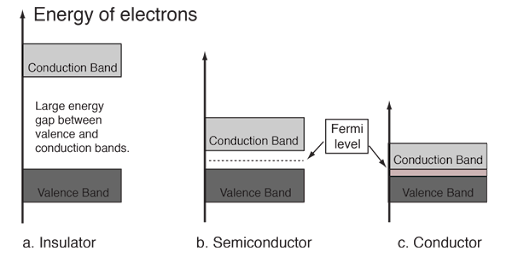
\includegraphics[width=.7\linewidth]{chapters/interatomic_potential_fitting/images/energy-bands-hyperphysics.png}
    \caption{Energy gap between valence and conduction bands\cite{bandgapshyperphysics}}
    \label{fig:bandgapshyperphysics}
\end{minipage}
\end{figure}

Fermi-Dirac statistics determine the probability of a Fermion having an energy E (eq. \ref{eq:fermidirac}).  As the temperature increases the probability of finding a fermion above the Fermi energy increases (fig. \ref{fig:fermidiracdist}).  This also smooths the discontinuity at the Fermi surface between the occupied and unoccupied states (at 0K). 

\begin{equation}
\begin{split}
F(E) = \frac{1}{\exp(\frac{E - E_F}{kT}) + 1}
\end{split}
\label{eq:fermidirac}
\end{equation}

\begin{figure}
\centering
\begin{minipage}{.65\textwidth}
\centering
    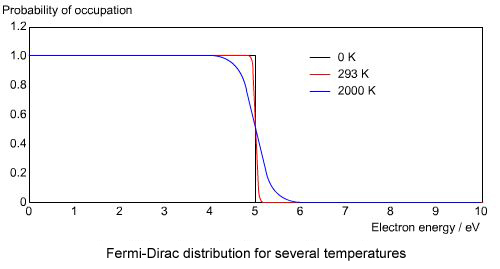
\includegraphics[width=.7\linewidth]{chapters/interatomic_potential_fitting/images/fermiDirac.jpg}
    \caption{Probability F(E) of finding a fermion with energy E at several temperatures\cite{fermidiracdist}}
    \label{fig:fermidiracdist}
\end{minipage}
\end{figure}

To avoid having to integrate the \acrshort{bz} with a very fine mesh, a smearing function is introduced to remove the discontinuity at the Fermi surface, making the integral over the \acrshort{bz} differentiable at every point.  The relationship between the delta and Heaviside step is used to replace the step function when integrated (eq. \ref{eq:deltaheaviside}).

\begin{equation}
\begin{split}
\int_{-\infty}^{\infty} \delta(k)dk = \Theta(x)
\end{split}
\label{eq:deltaheaviside}
\end{equation}

\begin{equation}
\begin{split}
I = \int_{-\infty}^{\infty} S(\epsilon-E_F) \int_{BZ} f(\vec{k}) \delta(\epsilon - E(\vec{k})) d\vec{k} d\epsilon
\end{split}
\label{eq:stepintegral}
\end{equation}

The step function at the Fermi surface (eq. \ref{eq:stepintegral}), that causes the discontinuity, may be replaced with a smearing function\cite{methfesslpaxton}.  Four of these functions are available to use in the PWscf \acrshort{dft} code.

The Fermi-Dirac function, as mentioned above, is used to heat the system.  It removes the discontinuity but the \acrshort{scf} will converge to the wrong energy (eq. \ref{eq:fermidirac2}).

\begin{equation}
\begin{split}
S_{FD}(\epsilon) = \frac{1}{\exp(\frac{\epsilon - E_F}{kT}) + 1}
\end{split}
\label{eq:fermidirac2}
\end{equation}

A Gaussian smear is also used to replace the step function although, unlike the Fermi-Dirac function, it has no physical meaning (eq. \ref{eq:gaussiansmear}).

\begin{equation}
\begin{split}
S_{G}(\epsilon) = \frac{1}{2} \left[ 1 - \erf\left(\frac{\epsilon - \mu}{\sigma}\right)\right]
\end{split}
\label{eq:gaussiansmear}
\end{equation}

The Methfessel-Paxton method attempts to correct the errors introduced by the previous smearing functions where the delta function is replaced with Hermite polynomials (fig. \ref{fig:deltahermite} and eq. \ref{eq:methfesselpaxton}).  A drawback of this method is that is allows for negative occupancy of electron states\cite{marzarithesis1}.

\begin{figure}
\centering
\begin{minipage}{.65\textwidth}
\centering
    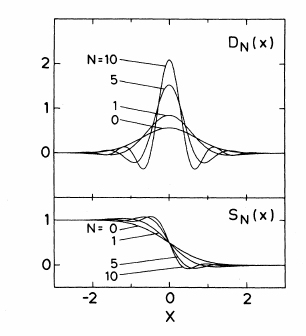
\includegraphics[width=.8\linewidth]{chapters/interatomic_potential_fitting/images/methfesselpaxton.png}
    \caption{Delta function replaced by successive Hermite polynomials\cite{methfesslpaxton}}
    \label{fig:deltahermite}
\end{minipage}
\end{figure}

\begin{equation}
\begin{split}
x = \epsilon - E_F \
S_{MP,N}(x) = \frac{1}{2} \left[1 - erf\left(x\right)\right] + \sum_{n=1}^{N} A_n H_{2n+1}(x)\exp(-x^2)\
A_n = \frac{(-1)^n}{n! 4^n \sqrt{\pi}}
\end{split}
\label{eq:methfesselpaxton}
\end{equation}

The Mazari-Vanderbilt function was developed to address the short falling of the Methfessel-Paxton function.  The occupancy where this function is used is always positive (fig. \ref{fig:marzarimethfessel}).

\begin{equation}
\begin{split}
x = \frac{\mu-\epsilon}{\sigma}
\delta(x) = \frac{1}{\sqrt{\pi}} \exp(-(x-(\frac{1}{\sqrt{2}}))^2) (2-\sqrt{2} x)
\end{split}
\label{eq:methfesselpaxton}
\end{equation}

\begin{figure}
\centering
\begin{minipage}{.65\textwidth}
\centering
    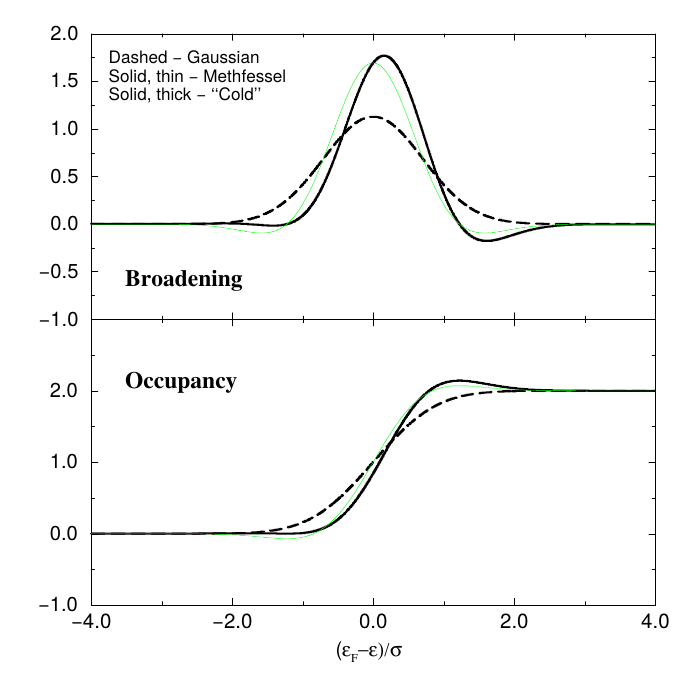
\includegraphics[width=.75\linewidth]{chapters/interatomic_potential_fitting/images/marzarismearing.png}
    \caption{The occupancy for the Marzari-Vanderbilt smearing function is always positive, unlike the Methfessl-Paxton function\cite{marzarithesis2}}
    \label{fig:marzarimethfessel}
\end{minipage}
\end{figure}

The recommended smearing function for Quantum Espresso is the Mazari-Vanderbilt type.  Dr Mazari
who co-developed the smearing type also contributed to the development of Quantum Espresso.  Dr Vanderbilt has researched condensed-matter physics for 30 years and an entire category of pseudopotentials is named after him.



\FloatBarrier
\subsection{Ferromagnetism, Antiferromagnetism and Hund's Rule}
\label{section:hundsrule}

Electrons are spin-half particles.  There isn't a classical analogue to spin, but it may (incorrectly) be imagined as a electron spinning and creating a magnetic field.  The electrons may also be (incorrectly) pictured as orbiting the nucleus.  This combination of orbital and intrinsic momentum give the total electronic angular momentum $\vec{J} = \vec{L} + \vec{S}$, and the total magnetic dipole moment is proportional to this.

Electrons fill the shells of a ground state atom such that the energy is minimised.  Four quantum numbers are used to describe electrons bound to an atom: n, l, $m_l$ and $m_s$.  The Pauli exclusion principle states that the electrons, which are fermions, cannot have the same quantum numbers as another electron bound to that atom.

Electrons may be spin up or spin down thus two electrons can have the same n, l, $m_l$ with two values for $m_s$ available.  The energy is minimised by not pairing up and down electrons until all the free slots due to the coulomb interaction between the electrons.  Once each slot contains one electron, they begin to pair.

The electronic configuration of \Gls{Fe} highlights this (eq \ref{eq:fullironconfiguration}).


\begin{equation}
\begin{split}
\text{Electronic configuration of Iron}\\
&1s^2 \:\:\:\: \underline{\uparrow \downarrow} \\
&2s^2 \:\:\:\: \underline{\uparrow \downarrow} \\
&2p^6 \:\:\:\: \underline{\uparrow \downarrow} \:\:\:\:  \underline{\uparrow  \downarrow} \:\:\:\:  \underline{\uparrow  \downarrow} \\
&3s^2 \:\:\:\: \underline{\uparrow \downarrow} \\
&3p^6 \:\:\:\: \underline{\uparrow \downarrow} \:\:\:\:  \underline{\uparrow \downarrow} \:\:\:\:  \underline{\uparrow \downarrow} \\
&4s^2 \:\:\:\: \underline{\uparrow \downarrow} \\
&3d^6 \:\:\:\: \underline{\uparrow \downarrow} \:\:\:\:  \underline{\uparrow \:\:} \:\:\:\:  \underline{\uparrow \:\:} \:\:\:\: \underline{\uparrow \:\:} \:\:\:\: \underline{\uparrow \:\:}\\
\end{split}
\label{eq:fullironconfiguration}
\end{equation}

Rather than fill the 3d shell from left to right, the first five slots take electrons with spin in the same direction, and the remaining electron fills the first slot with spin opposite to the first five electrons.

Being fermions the wavefunction for the two electrons must be antisymmetric, with spins opposite to one another.  Electrons with the same spin will repel one another and this causes an increase in the screening between the electrons and the nucleus.  The screening lowers the attraction between the electrons and the nucleus that then results in the total energy of the atom decreasing\cite{aligningelectrons}.

\begin{equation}
\begin{split}
\text{Electronic configuration of Chromium (outer shells)}\\
&4s^1 \:\:\:\:  \underline{\uparrow \:\:} \\
&3d^5 \:\:\:\:  \underline{\uparrow \:\:} \:\:\:\:  \underline{\uparrow \:\:} \:\:\:\:  \underline{\uparrow \:\:} \:\:\:\: \underline{\uparrow \:\:} \:\:\:\: \underline{\uparrow \:\:}
\end{split}
\label{eq:chromiumconfig}
\end{equation}

\begin{equation}
\begin{split}
\text{Electronic configuration of Iron (outer shells)}\\
&4s^2 \:\:\:\:  \underline{\uparrow \downarrow} \\
&3d^6 \:\:\:\:  \underline{\uparrow \downarrow} \:\:\:\:  \underline{\uparrow \:\:} \:\:\:\:  \underline{\uparrow \:\:} \:\:\:\: \underline{\uparrow \:\:} \:\:\:\: \underline{\uparrow \:\:}
\end{split}
\label{eq:ironconfig}
\end{equation}

\begin{equation}
\begin{split}
\text{Electronic configuration of Cobalt (outer shells)}\\
&4s^2 \:\:\:\:  \underline{\uparrow \downarrow} \\
&3d^7 \:\:\:\:  \underline{\uparrow \downarrow} \:\:\:\:  \underline{\uparrow  \downarrow} \:\:\:\:  \underline{\uparrow \:\:} \:\:\:\: \underline{\uparrow \:\:} \:\:\:\: \underline{\uparrow \:\:}
\end{split}
\label{eq:cobaltconfig}
\end{equation}

\begin{equation}
\begin{split}
\text{Electronic configuration of Nickel (outer shells)}\\
&4s^2 \:\:\:\:  \underline{\uparrow \downarrow} \\
&3d^8 \:\:\:\:  \underline{\uparrow \downarrow} \:\:\:\:  \underline{\uparrow  \downarrow} \:\:\:\:  \underline{\uparrow  \downarrow} \:\:\:\: \underline{\uparrow \:\:} \:\:\:\: \underline{\uparrow \:\:}
\end{split}
\label{eq:nickelconfig}
\end{equation}

In pure \Gls{Fe} (eq. \ref{eq:ironconfig}), under normal conditions, it is energetically favourable for the atoms to align in the same direction, and as such \Gls{Fe} is ferromagnetic.  \Gls{Co} (eq. \ref{eq:cobaltconfig}) has a \acrlong{cph} structure at room temperature.  It has a similar electronic structure to iron, but has three unpaired electrons in the 3d shell rather than four.  It is a ferromagnetic whilst it remains in its \acrshort{cph} form.  \Gls{Ni} (eq. \ref{eq:nickelconfig}) is also ferromagnetic, but it is ferromagnetic in its \acrshort{fcc} phase.

In its gamma phase, as it is in austenitic stainless steel, \Gls{Fe} atoms align opposite to one another in an antiferromagnetic arrangement.  This is also the same for \acrshort{bcc} \Gls{Cr} (eq. \ref{eq:chromiumconfig})  which is antiferromagnetic in its pure form under normal conditions.

 





\subsection{Collinear and Non-Collinear DFT Calculations}

Although briefly discussed by Kohn and Sham in their 1965 paper\cite{kohnsham}, \acrshort{dft} does not differentiate between the spins of electrons.  However, where the material is in a magnetic field, or where there are unpaired electrons, spin-\acrshort{dft} may be used.  This is a good way to model magnetic materials, such as iron, where Hund's rule leads to unpaired electrons as discussed in section \ref{section:hundsrule}.  

In collinear calculations the spin of electrons is restricted to two directions, up and down (in the z-axis, in the case of Quantum Espresso), whereas noncollinear calculations give the freedom to orient in any direction. 

\begin{equation}
\left( -\frac{1}{2} \nabla^2 + v_{n-e}(\vec{r_e}, \vec{r_n}) + \int d^3\vec{r'} \frac{\rho(\vec{r_{e}'})}{\lvert \vec{r_{e}} - \vec{r_{e}'} \rvert } + v_{xc}[\rho](\vec{r_{e}}) \right) \psi_{i} = E_{i} \psi_{i}
\label{eq:eqKS3}
\end{equation}

The Kohn-Sham equation is modified to include the magnetic field $B(\vec{r})$ and magnetization density $m(\vec{r})$\cite{spindft1}\cite{spindft2}.  Starting with the traditional Kohn-Sham equation, eq. \ref{eq:eqKS3}, the potential and densities are replaced with 2x2 matrices and the equation as a whole is split into spin up and spin down.

\begin{equation}
\begin{split}
\left(\left(-\frac{1}{2} \nabla^2  + \int d^3\vec{r'} \frac{\rho(\vec{r_{e}'})}{\lvert \vec{r_{e}} - \vec{r_{e}'} \rvert} \right) \begin{bmatrix} 1 & 0 \\ 0 & 1 \end{bmatrix} + \vec{v}_{n-e}(\vec{r_e}, \vec{r_n}) + v_{xc}[\vec{\rho}](\vec{r_{e}}) \right) \begin{bmatrix} \psi^{\uparrow}_{i} \\ \psi^{\downarrow}_{i} \end{bmatrix} = E_i \begin{bmatrix} \psi^{\uparrow}_{i} \\ \psi^{\downarrow}_{i} \end{bmatrix} 
\label{eq:eqKSSDFT1}
\end{split}
\end{equation}

The equation is modified as shown in eq. \ref{eq:eqKSSDFT1} and, using the \gls{paulivector}, the potential functions (eq. \ref{eq:sdftdensity} and eq. \ref{eq:sdftpotential})\cite{spindft4} and density functions are rewritten (eq. \ref{eq:sdftpotentialxc})\cite{spindft4}.

\begin{equation}
\begin{split}
\vec{\rho}(\vec{r}) = \frac{1}{2} \begin{bmatrix} \rho(\vec{r}) + m_z(\vec{r}) & m_x(\vec{r}) - i m_y(\vec{r}) \\ m_x(\vec{r}) + i m_y(\vec{r}) & \rho(\vec{r}) - m_z(\vec{r}) \end{bmatrix}
\label{eq:sdftdensity}
\end{split}
\end{equation}

\begin{equation}
\begin{split}
\vec{v}(\vec{r}) = \begin{bmatrix} v(\vec{r}) + \mu_B B_z(\vec{r}) & \mu_B (B_x(\vec{r}) - i B_y(\vec{r})) \\ \mu_B (B_x(\vec{r}) + i B_y(\vec{r})) & v(\vec{r}) - \mu_B B_z(\vec{r}) \end{bmatrix}
\label{eq:sdftpotential}
\end{split}
\end{equation}

\begin{equation}
\begin{split}
\vec{v_{xc}}(\vec{r}) = \begin{bmatrix} v_{xc}(\vec{r}) + \mu_B B_{xc, z}(\vec{r}) & \mu_B (B_{xc, x}(\vec{r}) - i B_{xc, y}(\vec{r})) \\ \mu_B (B_{xc, x}(\vec{r}) + i B_{xc, y}(\vec{r})) & v_{xc}(\vec{r}) - \mu_B B_{xc, z}(\vec{r}) \end{bmatrix}
\label{eq:sdftpotentialxc}
\end{split}
\end{equation}

This work is only concerned with collinear calculations, where the spins are aligned up or down with respect to the z-axis.  The equation derived by Von Barth and Hedin may be simplified to give the pair of Kohn-Sham equations in eq. \ref{eq:eqKSSDFT2}.

\begin{equation}
\begin{split}
\left(-\frac{1}{2} \nabla^2  + \int d^3\vec{r'} \frac{\rho(\vec{r_{e}'})}{\lvert \vec{r_{e}} - \vec{r_{e}'} \rvert} + v^{\uparrow}_{xc}[\vec{\rho}](\vec{r_{e}}) + B_{z}(\vec{r}) \right)\psi^{\uparrow}_{i}(\vec{r}) = E^{\uparrow}_i \psi^{\uparrow}_{i}(\vec{r})  \\
\left(-\frac{1}{2} \nabla^2  + \int d^3\vec{r'} \frac{\rho(\vec{r_{e}'})}{\lvert \vec{r_{e}} - \vec{r_{e}'} \rvert} + v^{\downarrow}_{xc}[\vec{\rho}](\vec{r_{e}}) - B_{z}(\vec{r}) \right)\psi^{\downarrow}_{i}(\vec{r}) = E^{\downarrow}_i \psi^{\downarrow}_{i}(\vec{r})
\label{eq:eqKSSDFT2}
\end{split}
\end{equation}

This model requires self consistently solving for both the charge density $\rho(\vec{r})$ and magnetisation density $m_{z}(\vec{r})$.  It will be adequate for modelling the ferromagnetism of pure iron and antiferromagnetic structure of iron as it exists in austenitic stainless steel.  A full non-collinear treatment would no doubt be better, when considering surfaces and the presence of doped \acrshort{pgm}s atoms in the structure, but would require more resources plus reliable and tested pseudopotentials suitable for these calculations.




